% **************************************************************************************************************
% A Classic Thesis Style
% An Homage to The Elements of Typographic Style
%
% Copyright (C) 2018 André Miede and Ivo Pletikosić
%
% If you like the style then I would appreciate a postcard. My address
% can be found in the file ClassicThesis.pdf. A collection of the
% postcards I received so far is available online at
% http://postcards.miede.de
%
% License:
% This program is free software; you can redistribute it and/or modify
% it under the terms of the GNU General Public License as published by
% the Free Software Foundation; either version 2 of the License, or
% (at your option) any later version.
%
% This program is distributed in the hope that it will be useful,
% but WITHOUT ANY WARRANTY; without even the implied warranty of
% MERCHANTABILITY or FITNESS FOR A PARTICULAR PURPOSE.  See the
% GNU General Public License for more details.
%
% You should have received a copy of the GNU General Public License
% along with this program; see the file COPYING.  If not, write to
% the Free Software Foundation, Inc., 59 Temple Place - Suite 330,
% Boston, MA 02111-1307, USA.
%
% PLEASE SEE ALSO THE AUTHORS' NOTE REGARDING THIS LICENSE
% IN THE DOCUMENTATION (ClassicThesis.pdf --> Chapter 1 / Chapter01.tex)
% **************************************************************************************************************
\RequirePackage{silence} % :-\
    \WarningFilter{scrreprt}{Usage of package `titlesec'}
    %\WarningFilter{scrreprt}{Activating an ugly workaround}
    \WarningFilter{titlesec}{Non standard sectioning command detected}
\documentclass[ twoside,openright,titlepage,numbers=noenddot,%1headlines,
                headinclude,footinclude,cleardoublepage=empty,abstract=on,
                BCOR=5mm,paper=a4,fontsize=11pt
                ]{scrreprt}

%********************************************************************
% Note: Make all your adjustments in here
%*******************************************************
% ****************************************************************************************************
% classicthesis-config.tex
% formerly known as loadpackages.sty, classicthesis-ldpkg.sty, and classicthesis-preamble.sty
% Use it at the beginning of your ClassicThesis.tex, or as a LaTeX Preamble
% in your ClassicThesis.{tex,lyx} with % ****************************************************************************************************
% classicthesis-config.tex
% formerly known as loadpackages.sty, classicthesis-ldpkg.sty, and classicthesis-preamble.sty
% Use it at the beginning of your ClassicThesis.tex, or as a LaTeX Preamble
% in your ClassicThesis.{tex,lyx} with % ****************************************************************************************************
% classicthesis-config.tex
% formerly known as loadpackages.sty, classicthesis-ldpkg.sty, and classicthesis-preamble.sty
% Use it at the beginning of your ClassicThesis.tex, or as a LaTeX Preamble
% in your ClassicThesis.{tex,lyx} with \input{classicthesis-config}
% ****************************************************************************************************
% If you like the classicthesis, then I would appreciate a postcard.
% My address can be found in the file ClassicThesis.pdf. A collection
% of the postcards I received so far is available online at
% http://postcards.miede.de
% ****************************************************************************************************


% ****************************************************************************************************
% 0. Set the encoding of your files. UTF-8 is the only sensible encoding nowadays. If you can't read
% äöüßáéçèê∂åëæƒÏ€ then change the encoding setting in your editor, not the line below. If your editor
% does not support utf8 use another editor!
% ****************************************************************************************************
\PassOptionsToPackage{utf8}{inputenc}
  \usepackage{inputenc}

\PassOptionsToPackage{T1}{fontenc} % T2A for cyrillics
  \usepackage{fontenc}


% ****************************************************************************************************
% 1. Configure classicthesis for your needs here, e.g., remove "drafting" below
% in order to deactivate the time-stamp on the pages
% (see ClassicThesis.pdf for more information):
% ****************************************************************************************************
\PassOptionsToPackage{
  drafting=true,    % print version information on the bottom of the pages
  tocaligned=false, % the left column of the toc will be aligned (no indentation)
  dottedtoc=false,  % page numbers in ToC flushed right
  eulerchapternumbers=true, % use AMS Euler for chapter font (otherwise Palatino)
  linedheaders=false,       % chaper headers will have line above and beneath
  floatperchapter=true,     % numbering per chapter for all floats (i.e., Figure 1.1)
  eulermath=false,  % use awesome Euler fonts for mathematical formulae (only with pdfLaTeX)
  beramono=true,    % toggle a nice monospaced font (w/ bold)
  palatino=true,    % deactivate standard font for loading another one, see the last section at the end of this file for suggestions
  style=classicthesis % classicthesis, arsclassica
}{classicthesis}


% ****************************************************************************************************
% 2. Personal data and user ad-hoc commands (insert your own data here)
% ****************************************************************************************************
\newcommand{\myTitle}{Normalizing FlashSim\xspace}
\newcommand{\mySubtitle}{A Deep Learning approach to the HEP simulation problem\xspace}
\newcommand{\myDegree}{Doktor-Ingenieur (Dr.-Ing.)\xspace}
\newcommand{\myName}{Francesco Vaselli\xspace}
\newcommand{\myProf}{Andrea Rizzi\xspace}
\newcommand{\myOtherProf}{Put name here\xspace}
\newcommand{\mySupervisor}{Andrea Rizzi\xspace}
\newcommand{\myFaculty}{Put data here\xspace}
\newcommand{\myDepartment}{Department of Physics, E. Fermi\xspace}
\newcommand{\myUni}{University of Pisa\xspace}
\newcommand{\myLocation}{Pisa\xspace}
\newcommand{\myTime}{September 2022\xspace}
\newcommand{\myVersion}{\classicthesis}

% ********************************************************************
% Setup, finetuning, and useful commands
% ********************************************************************
\providecommand{\mLyX}{L\kern-.1667em\lower.25em\hbox{Y}\kern-.125emX\@}
\newcommand{\ie}{i.\,e.}
\newcommand{\Ie}{I.\,e.}
\newcommand{\eg}{e.\,g.}
\newcommand{\Eg}{E.\,g.}
% ****************************************************************************************************


% ****************************************************************************************************
% 3. Loading some handy packages
% ****************************************************************************************************
% ********************************************************************
% Packages with options that might require adjustments
% ********************************************************************
\PassOptionsToPackage{ngerman,american}{babel} % change this to your language(s), main language last
% Spanish languages need extra options in order to work with this template
%\PassOptionsToPackage{spanish,es-lcroman}{babel}
    \usepackage{babel}

\usepackage{csquotes}
\PassOptionsToPackage{%
  %backend=biber,bibencoding=utf8, %instead of bibtex
  backend=bibtex8,bibencoding=ascii,%
  language=auto,%
  style=numeric-comp,%
  %style=authoryear-comp, % Author 1999, 2010
  %bibstyle=authoryear,dashed=false, % dashed: substitute rep. author with ---
  sorting=nyt, % name, year, title
  maxbibnames=10, % default: 3, et al.
  %backref=true,%
  natbib=true % natbib compatibility mode (\citep and \citet still work)
}{biblatex}
    \usepackage{biblatex}

\PassOptionsToPackage{fleqn}{amsmath}       % math environments and more by the AMS
  \usepackage{amsmath}

% ********************************************************************
% General useful packages
% ********************************************************************
\usepackage{graphicx} %
\usepackage{scrhack} % fix warnings when using KOMA with listings package
\usepackage{xspace} % to get the spacing after macros right
\PassOptionsToPackage{printonlyused,smaller}{acronym}
  \usepackage{acronym} % nice macros for handling all acronyms in the thesis
  %\renewcommand{\bflabel}[1]{{#1}\hfill} % fix the list of acronyms --> no longer working
  %\renewcommand*{\acsfont}[1]{\textsc{#1}}
  %\renewcommand*{\aclabelfont}[1]{\acsfont{#1}}
  %\def\bflabel#1{{#1\hfill}}
  \def\bflabel#1{{\acsfont{#1}\hfill}}
  \def\aclabelfont#1{\acsfont{#1}}
% ****************************************************************************************************
%\usepackage{pgfplots} % External TikZ/PGF support (thanks to Andreas Nautsch)
%\usetikzlibrary{external}
%\tikzexternalize[mode=list and make, prefix=ext-tikz/]
% ****************************************************************************************************


% ****************************************************************************************************
% 4. Setup floats: tables, (sub)figures, and captions as well as oultines
% ****************************************************************************************************
\usepackage{tabularx} % better tables
  \setlength{\extrarowheight}{3pt} % increase table row height
\newcommand{\tableheadline}[1]{\multicolumn{1}{l}{\spacedlowsmallcaps{#1}}}
\newcommand{\myfloatalign}{\centering} % to be used with each float for alignment
\usepackage{subfig}
\usepackage{outlines}
% ****************************************************************************************************

% ****************************************************************************************************
% tikz stuff
% ****************************************************************************************************
% \usepackage{tikz}
% \usetikzlibrary{matrix,chains,positioning,decorations.pathreplacing,arrows}
% \tikzset{basic/.style={draw,text width=1em,text badly centered}}
% \tikzset{functions/.style={basic,circle}}
% ****************************************************************************************************

% ****************************************************************************************************
% 5. Setup code listings
% ****************************************************************************************************
\usepackage{listings}
%\lstset{emph={trueIndex,root},emphstyle=\color{BlueViolet}}%\underbar} % for special keywords
\lstset{language=[LaTeX]Tex,%C++,
  morekeywords={PassOptionsToPackage,selectlanguage},
  keywordstyle=\color{RoyalBlue},%\bfseries,
  basicstyle=\small\ttfamily,
  %identifierstyle=\color{NavyBlue},
  commentstyle=\color{Green}\ttfamily,
  stringstyle=\rmfamily,
  numbers=none,%left,%
  numberstyle=\scriptsize,%\tiny
  stepnumber=5,
  numbersep=8pt,
  showstringspaces=false,
  breaklines=true,
  %frameround=ftff,
  %frame=single,
  belowcaptionskip=.75\baselineskip
  %frame=L
}
% ****************************************************************************************************




% ****************************************************************************************************
% 6. Last calls before the bar closes
% ****************************************************************************************************
% ********************************************************************
% Her Majesty herself
% ********************************************************************
\usepackage{classicthesis}


% ********************************************************************
% Fine-tune hyperreferences (hyperref should be called last)
% ********************************************************************
\hypersetup{%
  %draft, % hyperref's draft mode, for printing see below
  colorlinks=true, linktocpage=true, pdfstartpage=3, pdfstartview=FitV,%
  % uncomment the following line if you want to have black links (e.g., for printing)
  %colorlinks=false, linktocpage=false, pdfstartpage=3, pdfstartview=FitV, pdfborder={0 0 0},%
  breaklinks=true, pageanchor=true,%
  pdfpagemode=UseNone, %
  % pdfpagemode=UseOutlines,%
  plainpages=false, bookmarksnumbered, bookmarksopen=true, bookmarksopenlevel=1,%
  hypertexnames=true, pdfhighlight=/O,%nesting=true,%frenchlinks,%
  urlcolor=CTurl, linkcolor=CTlink, citecolor=CTcitation, %pagecolor=RoyalBlue,%
  %urlcolor=Black, linkcolor=Black, citecolor=Black, %pagecolor=Black,%
  pdftitle={\myTitle},%
  pdfauthor={\textcopyright\ \myName, \myUni, \myFaculty},%
  pdfsubject={},%
  pdfkeywords={},%
  pdfcreator={pdfLaTeX},%
  pdfproducer={LaTeX with hyperref and classicthesis}%
}


% ********************************************************************
% Setup autoreferences (hyperref and babel)
% ********************************************************************
% There are some issues regarding autorefnames
% http://www.tex.ac.uk/cgi-bin/texfaq2html?label=latexwords
% you have to redefine the macros for the
% language you use, e.g., american, ngerman
% (as chosen when loading babel/AtBeginDocument)
% ********************************************************************
\makeatletter
\@ifpackageloaded{babel}%
  {%
    \addto\extrasamerican{%
      \renewcommand*{\figureautorefname}{Figure}%
      \renewcommand*{\tableautorefname}{Table}%
      \renewcommand*{\partautorefname}{Part}%
      \renewcommand*{\chapterautorefname}{Chapter}%
      \renewcommand*{\sectionautorefname}{Section}%
      \renewcommand*{\subsectionautorefname}{Section}%
      \renewcommand*{\subsubsectionautorefname}{Section}%
    }%
    \addto\extrasngerman{%
      \renewcommand*{\paragraphautorefname}{Absatz}%
      \renewcommand*{\subparagraphautorefname}{Unterabsatz}%
      \renewcommand*{\footnoteautorefname}{Fu\"snote}%
      \renewcommand*{\FancyVerbLineautorefname}{Zeile}%
      \renewcommand*{\theoremautorefname}{Theorem}%
      \renewcommand*{\appendixautorefname}{Anhang}%
      \renewcommand*{\equationautorefname}{Gleichung}%
      \renewcommand*{\itemautorefname}{Punkt}%
    }%
      % Fix to getting autorefs for subfigures right (thanks to Belinda Vogt for changing the definition)
      \providecommand{\subfigureautorefname}{\figureautorefname}%
    }{\relax}
\makeatother


% ********************************************************************
% Development Stuff
% ********************************************************************
\listfiles
%\PassOptionsToPackage{l2tabu,orthodox,abort}{nag}
%  \usepackage{nag}
%\PassOptionsToPackage{warning, all}{onlyamsmath}
%  \usepackage{onlyamsmath}


% ****************************************************************************************************
% 7. Further adjustments (experimental)
% ****************************************************************************************************
% ********************************************************************
% Changing the text area
% ********************************************************************
%\areaset[current]{312pt}{761pt} % 686 (factor 2.2) + 33 head + 42 head \the\footskip
%\setlength{\marginparwidth}{7em}%
%\setlength{\marginparsep}{2em}%

% ********************************************************************
% Using different fonts
% ********************************************************************
%\usepackage[oldstylenums]{kpfonts} % oldstyle notextcomp
% \usepackage[osf]{libertine}
%\usepackage[light,condensed,math]{iwona}
%\renewcommand{\sfdefault}{iwona}
%\usepackage{lmodern} % <-- no osf support :-(
%\usepackage{cfr-lm} %
%\usepackage[urw-garamond]{mathdesign} <-- no osf support :-(
%\usepackage[default,osfigures]{opensans} % scale=0.95
%\usepackage[sfdefault]{FiraSans}
% \usepackage[opticals,mathlf]{MinionPro} % onlytext
% ********************************************************************
%\usepackage[largesc,osf]{newpxtext}
%\linespread{1.05} % a bit more for Palatino
% Used to fix these:
% https://bitbucket.org/amiede/classicthesis/issues/139/italics-in-pallatino-capitals-chapter
% https://bitbucket.org/amiede/classicthesis/issues/45/problema-testatine-su-classicthesis-style
% ********************************************************************
% ****************************************************************************************************

% ****************************************************************************************************
% tikz stuff
% ****************************************************************************************************
\usepackage{tikz}
\usetikzlibrary{calc, fit, matrix,chains,positioning,decorations.pathreplacing,arrows}
\tikzset{basic/.style={draw,text width=1em,text badly centered}}
\tikzset{functions/.style={basic,circle}}
\usepackage{neuralnetwork}
\usepackage{xstring}

\newcommand\drawNodes[2]{
  % #1 (str): namespace
  % #2 (list[list[str]]): list of labels to print in the node of each neuron
  \foreach \neurons [count=\lyrIdx] in #2 {
    \StrCount{\neurons}{,}[\lyrLength] % use xstring package to save each layer size into \lyrLength macro
    \foreach \n [count=\nIdx] in \neurons
      \node[neuron] (#1-\lyrIdx-\nIdx) at (2*\lyrIdx, \lyrLength/2-1.4*\nIdx) {\n};
  }
}

\newcommand\denselyConnectNodes[2]{
  % #1 (str): namespace
  % #2 (list[int]): number of nodes in each layer
  \foreach \n [count=\lyrIdx, remember=\lyrIdx as \previdx, remember=\n as \prevn] in #2 {
    \foreach \y in {1,...,\n} {
      \ifnum \lyrIdx > 1
        \foreach \x in {1,...,\prevn}
          \draw[->] (#1-\previdx-\x) -- (#1-\lyrIdx-\y);
      \fi
    }
  }
}

% ****************************************************************************************************
% ****************************************************************************************************
% If you like the classicthesis, then I would appreciate a postcard.
% My address can be found in the file ClassicThesis.pdf. A collection
% of the postcards I received so far is available online at
% http://postcards.miede.de
% ****************************************************************************************************


% ****************************************************************************************************
% 0. Set the encoding of your files. UTF-8 is the only sensible encoding nowadays. If you can't read
% äöüßáéçèê∂åëæƒÏ€ then change the encoding setting in your editor, not the line below. If your editor
% does not support utf8 use another editor!
% ****************************************************************************************************
\PassOptionsToPackage{utf8}{inputenc}
  \usepackage{inputenc}

\PassOptionsToPackage{T1}{fontenc} % T2A for cyrillics
  \usepackage{fontenc}


% ****************************************************************************************************
% 1. Configure classicthesis for your needs here, e.g., remove "drafting" below
% in order to deactivate the time-stamp on the pages
% (see ClassicThesis.pdf for more information):
% ****************************************************************************************************
\PassOptionsToPackage{
  drafting=true,    % print version information on the bottom of the pages
  tocaligned=false, % the left column of the toc will be aligned (no indentation)
  dottedtoc=false,  % page numbers in ToC flushed right
  eulerchapternumbers=true, % use AMS Euler for chapter font (otherwise Palatino)
  linedheaders=false,       % chaper headers will have line above and beneath
  floatperchapter=true,     % numbering per chapter for all floats (i.e., Figure 1.1)
  eulermath=false,  % use awesome Euler fonts for mathematical formulae (only with pdfLaTeX)
  beramono=true,    % toggle a nice monospaced font (w/ bold)
  palatino=true,    % deactivate standard font for loading another one, see the last section at the end of this file for suggestions
  style=classicthesis % classicthesis, arsclassica
}{classicthesis}


% ****************************************************************************************************
% 2. Personal data and user ad-hoc commands (insert your own data here)
% ****************************************************************************************************
\newcommand{\myTitle}{Normalizing FlashSim\xspace}
\newcommand{\mySubtitle}{A Deep Learning approach to the HEP simulation problem\xspace}
\newcommand{\myDegree}{Doktor-Ingenieur (Dr.-Ing.)\xspace}
\newcommand{\myName}{Francesco Vaselli\xspace}
\newcommand{\myProf}{Andrea Rizzi\xspace}
\newcommand{\myOtherProf}{Put name here\xspace}
\newcommand{\mySupervisor}{Andrea Rizzi\xspace}
\newcommand{\myFaculty}{Put data here\xspace}
\newcommand{\myDepartment}{Department of Physics, E. Fermi\xspace}
\newcommand{\myUni}{University of Pisa\xspace}
\newcommand{\myLocation}{Pisa\xspace}
\newcommand{\myTime}{September 2022\xspace}
\newcommand{\myVersion}{\classicthesis}

% ********************************************************************
% Setup, finetuning, and useful commands
% ********************************************************************
\providecommand{\mLyX}{L\kern-.1667em\lower.25em\hbox{Y}\kern-.125emX\@}
\newcommand{\ie}{i.\,e.}
\newcommand{\Ie}{I.\,e.}
\newcommand{\eg}{e.\,g.}
\newcommand{\Eg}{E.\,g.}
% ****************************************************************************************************


% ****************************************************************************************************
% 3. Loading some handy packages
% ****************************************************************************************************
% ********************************************************************
% Packages with options that might require adjustments
% ********************************************************************
\PassOptionsToPackage{ngerman,american}{babel} % change this to your language(s), main language last
% Spanish languages need extra options in order to work with this template
%\PassOptionsToPackage{spanish,es-lcroman}{babel}
    \usepackage{babel}

\usepackage{csquotes}
\PassOptionsToPackage{%
  %backend=biber,bibencoding=utf8, %instead of bibtex
  backend=bibtex8,bibencoding=ascii,%
  language=auto,%
  style=numeric-comp,%
  %style=authoryear-comp, % Author 1999, 2010
  %bibstyle=authoryear,dashed=false, % dashed: substitute rep. author with ---
  sorting=nyt, % name, year, title
  maxbibnames=10, % default: 3, et al.
  %backref=true,%
  natbib=true % natbib compatibility mode (\citep and \citet still work)
}{biblatex}
    \usepackage{biblatex}

\PassOptionsToPackage{fleqn}{amsmath}       % math environments and more by the AMS
  \usepackage{amsmath}

% ********************************************************************
% General useful packages
% ********************************************************************
\usepackage{graphicx} %
\usepackage{scrhack} % fix warnings when using KOMA with listings package
\usepackage{xspace} % to get the spacing after macros right
\PassOptionsToPackage{printonlyused,smaller}{acronym}
  \usepackage{acronym} % nice macros for handling all acronyms in the thesis
  %\renewcommand{\bflabel}[1]{{#1}\hfill} % fix the list of acronyms --> no longer working
  %\renewcommand*{\acsfont}[1]{\textsc{#1}}
  %\renewcommand*{\aclabelfont}[1]{\acsfont{#1}}
  %\def\bflabel#1{{#1\hfill}}
  \def\bflabel#1{{\acsfont{#1}\hfill}}
  \def\aclabelfont#1{\acsfont{#1}}
% ****************************************************************************************************
%\usepackage{pgfplots} % External TikZ/PGF support (thanks to Andreas Nautsch)
%\usetikzlibrary{external}
%\tikzexternalize[mode=list and make, prefix=ext-tikz/]
% ****************************************************************************************************


% ****************************************************************************************************
% 4. Setup floats: tables, (sub)figures, and captions as well as oultines
% ****************************************************************************************************
\usepackage{tabularx} % better tables
  \setlength{\extrarowheight}{3pt} % increase table row height
\newcommand{\tableheadline}[1]{\multicolumn{1}{l}{\spacedlowsmallcaps{#1}}}
\newcommand{\myfloatalign}{\centering} % to be used with each float for alignment
\usepackage{subfig}
\usepackage{outlines}
% ****************************************************************************************************

% ****************************************************************************************************
% tikz stuff
% ****************************************************************************************************
% \usepackage{tikz}
% \usetikzlibrary{matrix,chains,positioning,decorations.pathreplacing,arrows}
% \tikzset{basic/.style={draw,text width=1em,text badly centered}}
% \tikzset{functions/.style={basic,circle}}
% ****************************************************************************************************

% ****************************************************************************************************
% 5. Setup code listings
% ****************************************************************************************************
\usepackage{listings}
%\lstset{emph={trueIndex,root},emphstyle=\color{BlueViolet}}%\underbar} % for special keywords
\lstset{language=[LaTeX]Tex,%C++,
  morekeywords={PassOptionsToPackage,selectlanguage},
  keywordstyle=\color{RoyalBlue},%\bfseries,
  basicstyle=\small\ttfamily,
  %identifierstyle=\color{NavyBlue},
  commentstyle=\color{Green}\ttfamily,
  stringstyle=\rmfamily,
  numbers=none,%left,%
  numberstyle=\scriptsize,%\tiny
  stepnumber=5,
  numbersep=8pt,
  showstringspaces=false,
  breaklines=true,
  %frameround=ftff,
  %frame=single,
  belowcaptionskip=.75\baselineskip
  %frame=L
}
% ****************************************************************************************************




% ****************************************************************************************************
% 6. Last calls before the bar closes
% ****************************************************************************************************
% ********************************************************************
% Her Majesty herself
% ********************************************************************
\usepackage{classicthesis}


% ********************************************************************
% Fine-tune hyperreferences (hyperref should be called last)
% ********************************************************************
\hypersetup{%
  %draft, % hyperref's draft mode, for printing see below
  colorlinks=true, linktocpage=true, pdfstartpage=3, pdfstartview=FitV,%
  % uncomment the following line if you want to have black links (e.g., for printing)
  %colorlinks=false, linktocpage=false, pdfstartpage=3, pdfstartview=FitV, pdfborder={0 0 0},%
  breaklinks=true, pageanchor=true,%
  pdfpagemode=UseNone, %
  % pdfpagemode=UseOutlines,%
  plainpages=false, bookmarksnumbered, bookmarksopen=true, bookmarksopenlevel=1,%
  hypertexnames=true, pdfhighlight=/O,%nesting=true,%frenchlinks,%
  urlcolor=CTurl, linkcolor=CTlink, citecolor=CTcitation, %pagecolor=RoyalBlue,%
  %urlcolor=Black, linkcolor=Black, citecolor=Black, %pagecolor=Black,%
  pdftitle={\myTitle},%
  pdfauthor={\textcopyright\ \myName, \myUni, \myFaculty},%
  pdfsubject={},%
  pdfkeywords={},%
  pdfcreator={pdfLaTeX},%
  pdfproducer={LaTeX with hyperref and classicthesis}%
}


% ********************************************************************
% Setup autoreferences (hyperref and babel)
% ********************************************************************
% There are some issues regarding autorefnames
% http://www.tex.ac.uk/cgi-bin/texfaq2html?label=latexwords
% you have to redefine the macros for the
% language you use, e.g., american, ngerman
% (as chosen when loading babel/AtBeginDocument)
% ********************************************************************
\makeatletter
\@ifpackageloaded{babel}%
  {%
    \addto\extrasamerican{%
      \renewcommand*{\figureautorefname}{Figure}%
      \renewcommand*{\tableautorefname}{Table}%
      \renewcommand*{\partautorefname}{Part}%
      \renewcommand*{\chapterautorefname}{Chapter}%
      \renewcommand*{\sectionautorefname}{Section}%
      \renewcommand*{\subsectionautorefname}{Section}%
      \renewcommand*{\subsubsectionautorefname}{Section}%
    }%
    \addto\extrasngerman{%
      \renewcommand*{\paragraphautorefname}{Absatz}%
      \renewcommand*{\subparagraphautorefname}{Unterabsatz}%
      \renewcommand*{\footnoteautorefname}{Fu\"snote}%
      \renewcommand*{\FancyVerbLineautorefname}{Zeile}%
      \renewcommand*{\theoremautorefname}{Theorem}%
      \renewcommand*{\appendixautorefname}{Anhang}%
      \renewcommand*{\equationautorefname}{Gleichung}%
      \renewcommand*{\itemautorefname}{Punkt}%
    }%
      % Fix to getting autorefs for subfigures right (thanks to Belinda Vogt for changing the definition)
      \providecommand{\subfigureautorefname}{\figureautorefname}%
    }{\relax}
\makeatother


% ********************************************************************
% Development Stuff
% ********************************************************************
\listfiles
%\PassOptionsToPackage{l2tabu,orthodox,abort}{nag}
%  \usepackage{nag}
%\PassOptionsToPackage{warning, all}{onlyamsmath}
%  \usepackage{onlyamsmath}


% ****************************************************************************************************
% 7. Further adjustments (experimental)
% ****************************************************************************************************
% ********************************************************************
% Changing the text area
% ********************************************************************
%\areaset[current]{312pt}{761pt} % 686 (factor 2.2) + 33 head + 42 head \the\footskip
%\setlength{\marginparwidth}{7em}%
%\setlength{\marginparsep}{2em}%

% ********************************************************************
% Using different fonts
% ********************************************************************
%\usepackage[oldstylenums]{kpfonts} % oldstyle notextcomp
% \usepackage[osf]{libertine}
%\usepackage[light,condensed,math]{iwona}
%\renewcommand{\sfdefault}{iwona}
%\usepackage{lmodern} % <-- no osf support :-(
%\usepackage{cfr-lm} %
%\usepackage[urw-garamond]{mathdesign} <-- no osf support :-(
%\usepackage[default,osfigures]{opensans} % scale=0.95
%\usepackage[sfdefault]{FiraSans}
% \usepackage[opticals,mathlf]{MinionPro} % onlytext
% ********************************************************************
%\usepackage[largesc,osf]{newpxtext}
%\linespread{1.05} % a bit more for Palatino
% Used to fix these:
% https://bitbucket.org/amiede/classicthesis/issues/139/italics-in-pallatino-capitals-chapter
% https://bitbucket.org/amiede/classicthesis/issues/45/problema-testatine-su-classicthesis-style
% ********************************************************************
% ****************************************************************************************************

% ****************************************************************************************************
% tikz stuff
% ****************************************************************************************************
\usepackage{tikz}
\usetikzlibrary{calc, fit, matrix,chains,positioning,decorations.pathreplacing,arrows}
\tikzset{basic/.style={draw,text width=1em,text badly centered}}
\tikzset{functions/.style={basic,circle}}
\usepackage{neuralnetwork}
\usepackage{xstring}

\newcommand\drawNodes[2]{
  % #1 (str): namespace
  % #2 (list[list[str]]): list of labels to print in the node of each neuron
  \foreach \neurons [count=\lyrIdx] in #2 {
    \StrCount{\neurons}{,}[\lyrLength] % use xstring package to save each layer size into \lyrLength macro
    \foreach \n [count=\nIdx] in \neurons
      \node[neuron] (#1-\lyrIdx-\nIdx) at (2*\lyrIdx, \lyrLength/2-1.4*\nIdx) {\n};
  }
}

\newcommand\denselyConnectNodes[2]{
  % #1 (str): namespace
  % #2 (list[int]): number of nodes in each layer
  \foreach \n [count=\lyrIdx, remember=\lyrIdx as \previdx, remember=\n as \prevn] in #2 {
    \foreach \y in {1,...,\n} {
      \ifnum \lyrIdx > 1
        \foreach \x in {1,...,\prevn}
          \draw[->] (#1-\previdx-\x) -- (#1-\lyrIdx-\y);
      \fi
    }
  }
}

% ****************************************************************************************************
% ****************************************************************************************************
% If you like the classicthesis, then I would appreciate a postcard.
% My address can be found in the file ClassicThesis.pdf. A collection
% of the postcards I received so far is available online at
% http://postcards.miede.de
% ****************************************************************************************************


% ****************************************************************************************************
% 0. Set the encoding of your files. UTF-8 is the only sensible encoding nowadays. If you can't read
% äöüßáéçèê∂åëæƒÏ€ then change the encoding setting in your editor, not the line below. If your editor
% does not support utf8 use another editor!
% ****************************************************************************************************
\PassOptionsToPackage{utf8}{inputenc}
  \usepackage{inputenc}

\PassOptionsToPackage{T1}{fontenc} % T2A for cyrillics
  \usepackage{fontenc}


% ****************************************************************************************************
% 1. Configure classicthesis for your needs here, e.g., remove "drafting" below
% in order to deactivate the time-stamp on the pages
% (see ClassicThesis.pdf for more information):
% ****************************************************************************************************
\PassOptionsToPackage{
  drafting=true,    % print version information on the bottom of the pages
  tocaligned=false, % the left column of the toc will be aligned (no indentation)
  dottedtoc=false,  % page numbers in ToC flushed right
  eulerchapternumbers=true, % use AMS Euler for chapter font (otherwise Palatino)
  linedheaders=false,       % chaper headers will have line above and beneath
  floatperchapter=true,     % numbering per chapter for all floats (i.e., Figure 1.1)
  eulermath=false,  % use awesome Euler fonts for mathematical formulae (only with pdfLaTeX)
  beramono=true,    % toggle a nice monospaced font (w/ bold)
  palatino=true,    % deactivate standard font for loading another one, see the last section at the end of this file for suggestions
  style=classicthesis % classicthesis, arsclassica
}{classicthesis}


% ****************************************************************************************************
% 2. Personal data and user ad-hoc commands (insert your own data here)
% ****************************************************************************************************
\newcommand{\myTitle}{Normalizing FlashSim\xspace}
\newcommand{\mySubtitle}{A Deep Learning approach to the HEP simulation problem\xspace}
\newcommand{\myDegree}{Doktor-Ingenieur (Dr.-Ing.)\xspace}
\newcommand{\myName}{Francesco Vaselli\xspace}
\newcommand{\myProf}{Andrea Rizzi\xspace}
\newcommand{\myOtherProf}{Put name here\xspace}
\newcommand{\mySupervisor}{Andrea Rizzi\xspace}
\newcommand{\myFaculty}{Put data here\xspace}
\newcommand{\myDepartment}{Department of Physics, E. Fermi\xspace}
\newcommand{\myUni}{University of Pisa\xspace}
\newcommand{\myLocation}{Pisa\xspace}
\newcommand{\myTime}{September 2022\xspace}
\newcommand{\myVersion}{\classicthesis}

% ********************************************************************
% Setup, finetuning, and useful commands
% ********************************************************************
\providecommand{\mLyX}{L\kern-.1667em\lower.25em\hbox{Y}\kern-.125emX\@}
\newcommand{\ie}{i.\,e.}
\newcommand{\Ie}{I.\,e.}
\newcommand{\eg}{e.\,g.}
\newcommand{\Eg}{E.\,g.}
% ****************************************************************************************************


% ****************************************************************************************************
% 3. Loading some handy packages
% ****************************************************************************************************
% ********************************************************************
% Packages with options that might require adjustments
% ********************************************************************
\PassOptionsToPackage{ngerman,american}{babel} % change this to your language(s), main language last
% Spanish languages need extra options in order to work with this template
%\PassOptionsToPackage{spanish,es-lcroman}{babel}
    \usepackage{babel}

\usepackage{csquotes}
\PassOptionsToPackage{%
  %backend=biber,bibencoding=utf8, %instead of bibtex
  backend=bibtex8,bibencoding=ascii,%
  language=auto,%
  style=numeric-comp,%
  %style=authoryear-comp, % Author 1999, 2010
  %bibstyle=authoryear,dashed=false, % dashed: substitute rep. author with ---
  sorting=nyt, % name, year, title
  maxbibnames=10, % default: 3, et al.
  %backref=true,%
  natbib=true % natbib compatibility mode (\citep and \citet still work)
}{biblatex}
    \usepackage{biblatex}

\PassOptionsToPackage{fleqn}{amsmath}       % math environments and more by the AMS
  \usepackage{amsmath}

% ********************************************************************
% General useful packages
% ********************************************************************
\usepackage{graphicx} %
\usepackage{scrhack} % fix warnings when using KOMA with listings package
\usepackage{xspace} % to get the spacing after macros right
\PassOptionsToPackage{printonlyused,smaller}{acronym}
  \usepackage{acronym} % nice macros for handling all acronyms in the thesis
  %\renewcommand{\bflabel}[1]{{#1}\hfill} % fix the list of acronyms --> no longer working
  %\renewcommand*{\acsfont}[1]{\textsc{#1}}
  %\renewcommand*{\aclabelfont}[1]{\acsfont{#1}}
  %\def\bflabel#1{{#1\hfill}}
  \def\bflabel#1{{\acsfont{#1}\hfill}}
  \def\aclabelfont#1{\acsfont{#1}}
% ****************************************************************************************************
%\usepackage{pgfplots} % External TikZ/PGF support (thanks to Andreas Nautsch)
%\usetikzlibrary{external}
%\tikzexternalize[mode=list and make, prefix=ext-tikz/]
% ****************************************************************************************************


% ****************************************************************************************************
% 4. Setup floats: tables, (sub)figures, and captions as well as oultines
% ****************************************************************************************************
\usepackage{tabularx} % better tables
  \setlength{\extrarowheight}{3pt} % increase table row height
\newcommand{\tableheadline}[1]{\multicolumn{1}{l}{\spacedlowsmallcaps{#1}}}
\newcommand{\myfloatalign}{\centering} % to be used with each float for alignment
\usepackage{subfig}
\usepackage{outlines}
% ****************************************************************************************************

% ****************************************************************************************************
% tikz stuff
% ****************************************************************************************************
% \usepackage{tikz}
% \usetikzlibrary{matrix,chains,positioning,decorations.pathreplacing,arrows}
% \tikzset{basic/.style={draw,text width=1em,text badly centered}}
% \tikzset{functions/.style={basic,circle}}
% ****************************************************************************************************

% ****************************************************************************************************
% 5. Setup code listings
% ****************************************************************************************************
\usepackage{listings}
%\lstset{emph={trueIndex,root},emphstyle=\color{BlueViolet}}%\underbar} % for special keywords
\lstset{language=[LaTeX]Tex,%C++,
  morekeywords={PassOptionsToPackage,selectlanguage},
  keywordstyle=\color{RoyalBlue},%\bfseries,
  basicstyle=\small\ttfamily,
  %identifierstyle=\color{NavyBlue},
  commentstyle=\color{Green}\ttfamily,
  stringstyle=\rmfamily,
  numbers=none,%left,%
  numberstyle=\scriptsize,%\tiny
  stepnumber=5,
  numbersep=8pt,
  showstringspaces=false,
  breaklines=true,
  %frameround=ftff,
  %frame=single,
  belowcaptionskip=.75\baselineskip
  %frame=L
}
% ****************************************************************************************************




% ****************************************************************************************************
% 6. Last calls before the bar closes
% ****************************************************************************************************
% ********************************************************************
% Her Majesty herself
% ********************************************************************
\usepackage{classicthesis}


% ********************************************************************
% Fine-tune hyperreferences (hyperref should be called last)
% ********************************************************************
\hypersetup{%
  %draft, % hyperref's draft mode, for printing see below
  colorlinks=true, linktocpage=true, pdfstartpage=3, pdfstartview=FitV,%
  % uncomment the following line if you want to have black links (e.g., for printing)
  %colorlinks=false, linktocpage=false, pdfstartpage=3, pdfstartview=FitV, pdfborder={0 0 0},%
  breaklinks=true, pageanchor=true,%
  pdfpagemode=UseNone, %
  % pdfpagemode=UseOutlines,%
  plainpages=false, bookmarksnumbered, bookmarksopen=true, bookmarksopenlevel=1,%
  hypertexnames=true, pdfhighlight=/O,%nesting=true,%frenchlinks,%
  urlcolor=CTurl, linkcolor=CTlink, citecolor=CTcitation, %pagecolor=RoyalBlue,%
  %urlcolor=Black, linkcolor=Black, citecolor=Black, %pagecolor=Black,%
  pdftitle={\myTitle},%
  pdfauthor={\textcopyright\ \myName, \myUni, \myFaculty},%
  pdfsubject={},%
  pdfkeywords={},%
  pdfcreator={pdfLaTeX},%
  pdfproducer={LaTeX with hyperref and classicthesis}%
}


% ********************************************************************
% Setup autoreferences (hyperref and babel)
% ********************************************************************
% There are some issues regarding autorefnames
% http://www.tex.ac.uk/cgi-bin/texfaq2html?label=latexwords
% you have to redefine the macros for the
% language you use, e.g., american, ngerman
% (as chosen when loading babel/AtBeginDocument)
% ********************************************************************
\makeatletter
\@ifpackageloaded{babel}%
  {%
    \addto\extrasamerican{%
      \renewcommand*{\figureautorefname}{Figure}%
      \renewcommand*{\tableautorefname}{Table}%
      \renewcommand*{\partautorefname}{Part}%
      \renewcommand*{\chapterautorefname}{Chapter}%
      \renewcommand*{\sectionautorefname}{Section}%
      \renewcommand*{\subsectionautorefname}{Section}%
      \renewcommand*{\subsubsectionautorefname}{Section}%
    }%
    \addto\extrasngerman{%
      \renewcommand*{\paragraphautorefname}{Absatz}%
      \renewcommand*{\subparagraphautorefname}{Unterabsatz}%
      \renewcommand*{\footnoteautorefname}{Fu\"snote}%
      \renewcommand*{\FancyVerbLineautorefname}{Zeile}%
      \renewcommand*{\theoremautorefname}{Theorem}%
      \renewcommand*{\appendixautorefname}{Anhang}%
      \renewcommand*{\equationautorefname}{Gleichung}%
      \renewcommand*{\itemautorefname}{Punkt}%
    }%
      % Fix to getting autorefs for subfigures right (thanks to Belinda Vogt for changing the definition)
      \providecommand{\subfigureautorefname}{\figureautorefname}%
    }{\relax}
\makeatother


% ********************************************************************
% Development Stuff
% ********************************************************************
\listfiles
%\PassOptionsToPackage{l2tabu,orthodox,abort}{nag}
%  \usepackage{nag}
%\PassOptionsToPackage{warning, all}{onlyamsmath}
%  \usepackage{onlyamsmath}


% ****************************************************************************************************
% 7. Further adjustments (experimental)
% ****************************************************************************************************
% ********************************************************************
% Changing the text area
% ********************************************************************
%\areaset[current]{312pt}{761pt} % 686 (factor 2.2) + 33 head + 42 head \the\footskip
%\setlength{\marginparwidth}{7em}%
%\setlength{\marginparsep}{2em}%

% ********************************************************************
% Using different fonts
% ********************************************************************
%\usepackage[oldstylenums]{kpfonts} % oldstyle notextcomp
% \usepackage[osf]{libertine}
%\usepackage[light,condensed,math]{iwona}
%\renewcommand{\sfdefault}{iwona}
%\usepackage{lmodern} % <-- no osf support :-(
%\usepackage{cfr-lm} %
%\usepackage[urw-garamond]{mathdesign} <-- no osf support :-(
%\usepackage[default,osfigures]{opensans} % scale=0.95
%\usepackage[sfdefault]{FiraSans}
% \usepackage[opticals,mathlf]{MinionPro} % onlytext
% ********************************************************************
%\usepackage[largesc,osf]{newpxtext}
%\linespread{1.05} % a bit more for Palatino
% Used to fix these:
% https://bitbucket.org/amiede/classicthesis/issues/139/italics-in-pallatino-capitals-chapter
% https://bitbucket.org/amiede/classicthesis/issues/45/problema-testatine-su-classicthesis-style
% ********************************************************************
% ****************************************************************************************************

% ****************************************************************************************************
% tikz stuff
% ****************************************************************************************************
\usepackage{tikz}
\usetikzlibrary{calc, fit, matrix,chains,positioning,decorations.pathreplacing,arrows}
\tikzset{basic/.style={draw,text width=1em,text badly centered}}
\tikzset{functions/.style={basic,circle}}
\usepackage{neuralnetwork}
\usepackage{xstring}

\newcommand\drawNodes[2]{
  % #1 (str): namespace
  % #2 (list[list[str]]): list of labels to print in the node of each neuron
  \foreach \neurons [count=\lyrIdx] in #2 {
    \StrCount{\neurons}{,}[\lyrLength] % use xstring package to save each layer size into \lyrLength macro
    \foreach \n [count=\nIdx] in \neurons
      \node[neuron] (#1-\lyrIdx-\nIdx) at (2*\lyrIdx, \lyrLength/2-1.4*\nIdx) {\n};
  }
}

\newcommand\denselyConnectNodes[2]{
  % #1 (str): namespace
  % #2 (list[int]): number of nodes in each layer
  \foreach \n [count=\lyrIdx, remember=\lyrIdx as \previdx, remember=\n as \prevn] in #2 {
    \foreach \y in {1,...,\n} {
      \ifnum \lyrIdx > 1
        \foreach \x in {1,...,\prevn}
          \draw[->] (#1-\previdx-\x) -- (#1-\lyrIdx-\y);
      \fi
    }
  }
}

% ****************************************************************************************************

%********************************************************************
% Bibliographies
%*******************************************************
\addbibresource{Bibliography.bib}
\addbibresource[label=ownpubs]{AMiede_Publications.bib}

%********************************************************************
% Hyphenation
%*******************************************************
%\hyphenation{put special hyphenation here}

% ********************************************************************
% GO!GO!GO! MOVE IT!
%*******************************************************
\begin{document}
\frenchspacing
\raggedbottom
\selectlanguage{american} % american ngerman
%\renewcommand*{\bibname}{new name}
%\setbibpreamble{}
\pagenumbering{roman}
\pagestyle{plain}
%********************************************************************
% Frontmatter
%*******************************************************
%%*******************************************************
% Little Dirty Titlepage
%*******************************************************
\thispagestyle{empty}
%\pdfbookmark[1]{Titel}{title}
%*******************************************************
\begin{center}
    \spacedlowsmallcaps{\myName} \\ \medskip

    \begingroup
        \color{CTtitle}\spacedallcaps{\myTitle}
    \endgroup
\end{center}

%*******************************************************
% Titlepage
%*******************************************************
\begin{titlepage}
    %\pdfbookmark[1]{\myTitle}{titlepage}
    % if you want the titlepage to be centered, uncomment and fine-tune the line below (KOMA classes environment)
    \begin{addmargin}[-1cm]{-3cm}
    \begin{center}
        \large

        \hfill

        \vfill

        \begingroup
            \color{CTtitle}\spacedallcaps{\myTitle} \\ \bigskip
        \endgroup

        \spacedlowsmallcaps{\myName}

        \vfill

        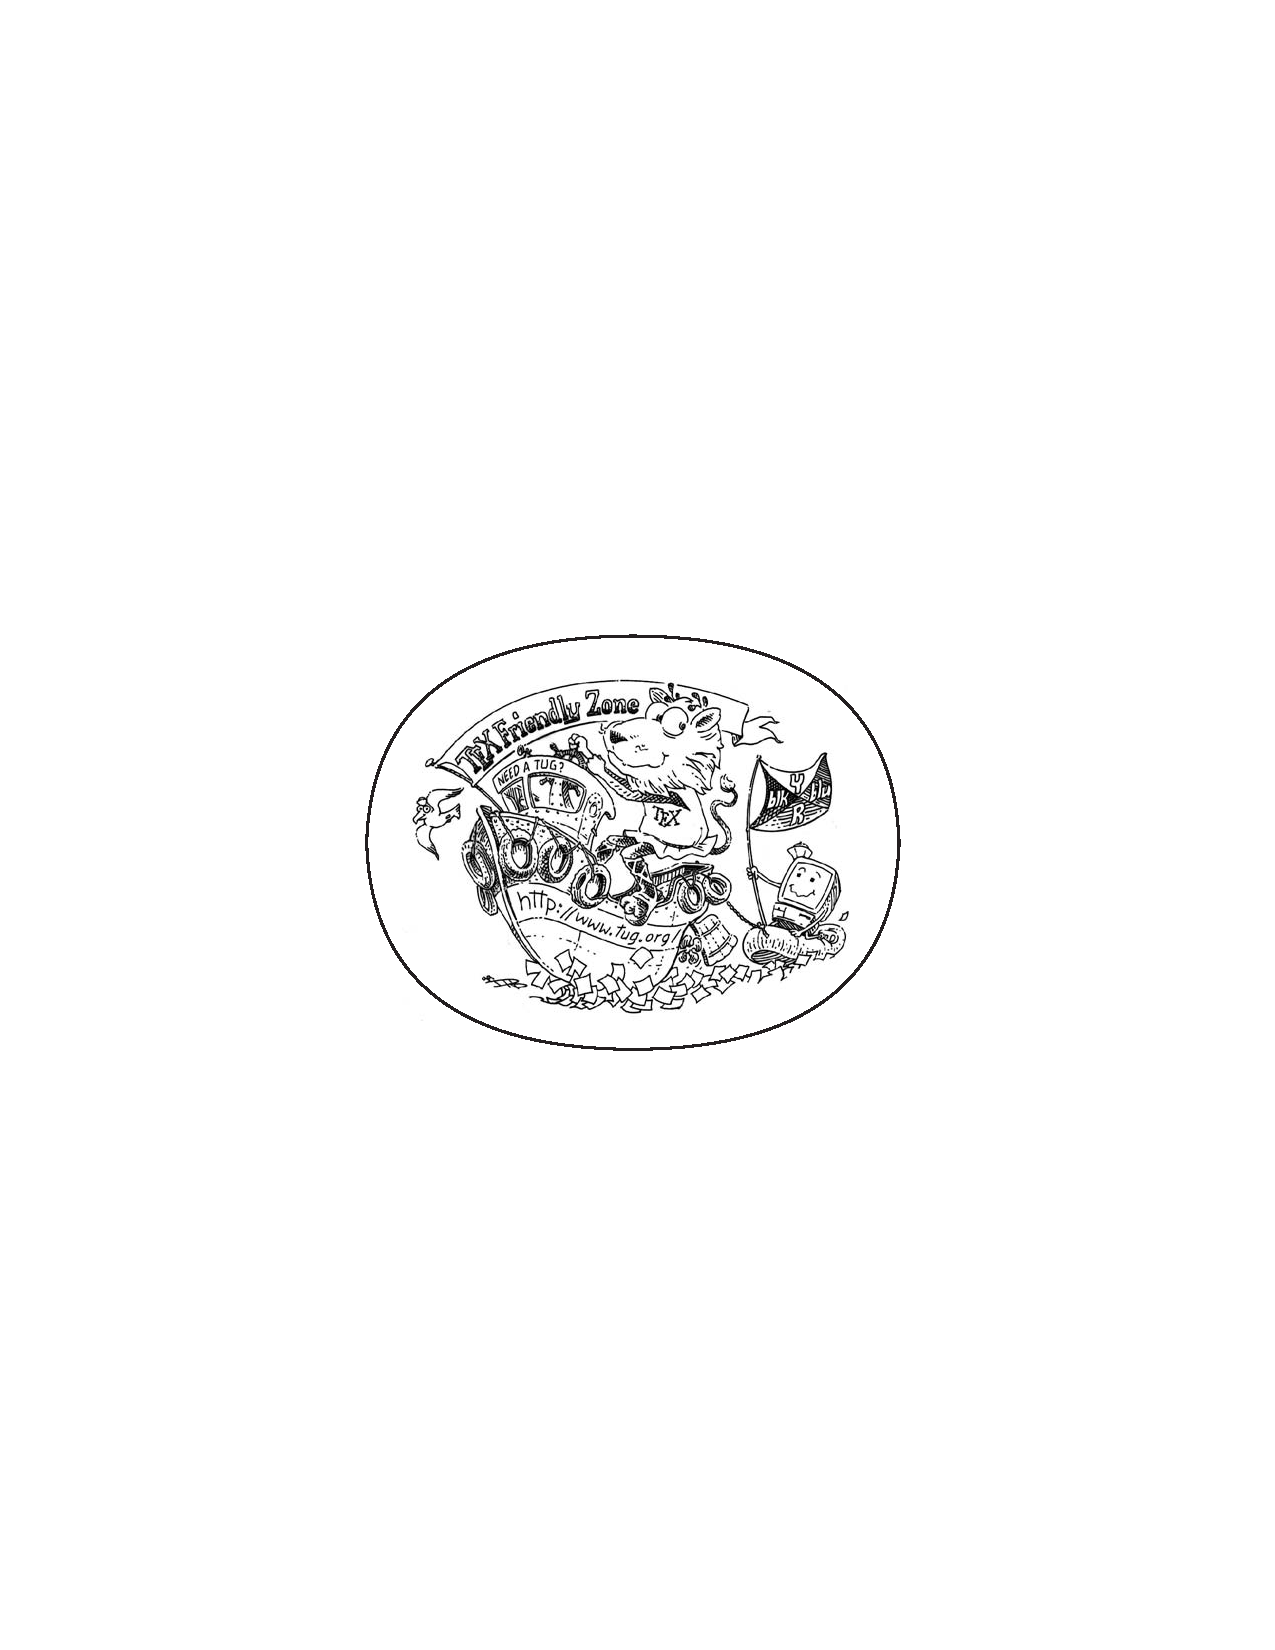
\includegraphics[width=6cm]{gfx/TFZsuperellipse_bw} \\ \medskip

        \mySubtitle \\ \medskip
        %\myDegree \\
        %\myDepartment \\
        %\myFaculty \\
        %\myUni \\ \bigskip

        \myTime\ -- \myVersion

        \vfill

    \end{center}
  \end{addmargin}
\end{titlepage}

\thispagestyle{empty}

\hfill

\vfill

\noindent\myName: \textit{\myTitle,} \mySubtitle, %\myDegree,
\textcopyright\ \myTime

%\bigskip
%
%\noindent\spacedlowsmallcaps{Supervisors}: \\
%\myProf \\
%\myOtherProf \\
%\mySupervisor
%
%\medskip
%
%\noindent\spacedlowsmallcaps{Location}: \\
%\myLocation
%
%\medskip
%
%\noindent\spacedlowsmallcaps{Time Frame}: \\
%\myTime

\cleardoublepage%*******************************************************
% Dedication
%*******************************************************
\thispagestyle{empty}
\phantomsection
\pdfbookmark[1]{Dedication}{Dedication}

\vspace*{3cm}

\begin{center}
    \emph{Ohana} means family. \\
    Family means nobody gets left behind, or forgotten. \\ \medskip
    --- Lilo \& Stitch
\end{center}

\medskip

\begin{center}
    Dedicated to the loving memory of Rudolf Miede. \\ \smallskip
    1939\,--\,2005
\end{center}

%\cleardoublepage\include{FrontBackmatter/Foreword}
\cleardoublepage%*******************************************************
% Abstract
%*******************************************************
%\renewcommand{\abstractname}{Abstract}
\pdfbookmark[1]{Abstract}{Abstract}
% \addcontentsline{toc}{chapter}{\tocEntry{Abstract}}
\begingroup
\let\clearpage\relax
\let\cleardoublepage\relax
\let\cleardoublepage\relax

\chapter*{Summary}
The necessity for \emph{computer-based simulations} is shared by many fields of physics. Specifically, in \emph{High Energy Physics} this necessity is of foremost importance, due to the complexity of the experiments and the vast amount of experimental data which are to be compared to theoretical models. However, starting from the physical calculations, the interaction with the detectors and the reconstruction of physical objects has proven to be extremely \emph{computationally expensive}. Because of this, current collaborations, such as the \emph{Compact Muon Solenoid} (CMS) one, are partially limited by the \emph{quantity} of simulated data available to them, as well by the available \emph{resources} to compute them in a reasonable time. As it has already been the case in countless applications, novel \emph{Machine Learning} (ML) techniques are expected to provide us with the much needed speed and accuracy, an expectation that we thoroughly investigated in the present work, at least for what concerns event simulation. The primary concern of this Thesis has been trying to build a prototype \emph{end-to-end sample analysis} generator, named \emph{FlashSim}.
The classical \emph{FullSim} approach starts from \emph{generator-level} particle listing; propagates stable particles through the detector and emulates the sensor and electronics response producing an output with the same level of detail and the same data representation as the actual detector. The FullSim output is then \emph{reconstructed} with the very same algorithms used on experimental data, calibrated in the same manner and finally transformed in a reduced format usable for the analysis--attempting to capture the changes in the properties of the originally simulated event. Working this way, we thus need to simulate $\approx 1$ MB of detector-like data per event, and then reduce it with the same algorithms used for actual data by a factor of 1000 (1 kB/ev) for analysis.
The key idea behind our work is that an accurate and fast prediction of the final reduction (1 kB/ev) can be achieved starting from the generator-level information alone through a ML approach skipping all intermediate steps.
As a first proof-of-concept, we simulated two classes of physical objects: \emph{jets} and \emph{muons}. This allowed us to put our results to the test in a real-world use case such as the preliminary analysis selection for VBF Channel of H$\rightarrow\mu^+\mu^-$, which mainly relies on those two types of objects.


The results are indeed confirming and possibly exceeding our initial expectation. Through the powerful ML technique of \emph{Normalizing Flows}, we simultaneously generate 22 key reconstructed variables for muons and 17 for jets, starting from \emph{random noise} and \emph{generator-level} physical inputs about the underlying process. The results are compared to the corresponding FullSim simulations results, based on the popular \texttt{Geant4} framework, showing optimal accuracy and preserving all the \emph{correlations} between variables pairs. 
The capacity of our approach to vary its outputs according to the specified physical content of an event is compared to the other major competing approach for fast simulation and it is found to be vastly superior. The proposed approach additionally demonstrates a raw generation speed of \emph{six orders of magnitude} greater than that of the FullSim approach, outputting events at a rate of 33,300 Hz instead of 1 event per minute. After introducing the preprocessing and postprocessing steps needed for a full end-to-end FlashSim generator, we apply it to a complete dataset consisting of different, previously unseen physical processes and we produce a full dataset ready to be used in the VBF H$\rightarrow\mu^+\mu^-$ analysis. We repeat the preliminary analysis selection performed by CMS in 2018, observing good agreement between selected-objects distributions. Additionally, when evaluating the actual \emph{Deep Neural Networks} used in the paper to perform the final signal fit, we obtain compatible outputs between our approach and FullSim, proving that the proposed approach can in fact be employed in a real-case scenario with a fraction of the time and the resources.
The current findings have the potential to completely change the approach to simulations at CMS and at the LHC, paving the way for online, on-demand generation of events. All these results point to interesting and rewarding directions for future research at the boundaries of high energy physics and machine learning.

This Thesis is structured into three parts:

Part 1 presents the context for our work, with Chapter 1 giving an overview of LHC, the CMS Experiment and its physics searches, focusing on the VBF Channel of H$\rightarrow\mu^+\mu^-$, later used as a realistic benchmark. Chapter 2 discusses the current approach to simulation, its costs and main limitations as well as presenting the standard CMS analysis format, the \emph{NanoAOD}.

Part 2 explains the ML tools employed as the backbone of our work, first in a broad and general introduction in Chapter 3 and then with a focus on Normalizing Flows during Chapter 4.

Part 3 presents the main, original contributions, discussing the implementation and the results in Chapter 5, showing the real analysis use case comparison in Chapter 6 and expanding on the conclusion and future outlook in Chapter 7. 
\endgroup

\vfill

%\cleardoublepage%*******************************************************
% Publications
%*******************************************************
\pdfbookmark[1]{Publications}{publications}
\chapter*{Publications}\graffito{This is just an early --~and currently ugly~-- test!}
This might come in handy for PhD theses: some ideas and figures have appeared previously in the following publications:

%\noindent Put your publications from the thesis here. The packages \texttt{multibib} or \texttt{bibtopic} etc. can be used to handle multiple different bibliographies in your document.

\begin{refsection}[ownpubs]
    \small
    \nocite{*} % is local to to the enclosing refsection
    \printbibliography[heading=none]
\end{refsection}

\emph{Attention}: This requires a separate run of \texttt{bibtex} for your \texttt{refsection}, \eg, \texttt{ClassicThesis1-blx} for this file. You might also use \texttt{biber} as the backend for \texttt{biblatex}. See also \url{http://tex.stackexchange.com/questions/128196/problem-with-refsection}.

\cleardoublepage%*******************************************************
% Acknowledgments
%*******************************************************
\pdfbookmark[1]{Acknowledgments}{acknowledgments}

\begin{flushright}{\slshape
    We have seen that computer programming is an art, \\
    because it applies accumulated knowledge to the world, \\
    because it requires skill and ingenuity, and especially \\
    because it produces objects of beauty.} \\ \medskip
    --- \defcitealias{knuth:1974}{Donald E. Knuth}\citetalias{knuth:1974} \citep{knuth:1974}
\end{flushright}



\bigskip

\begingroup
\let\clearpage\relax
\let\cleardoublepage\relax
\let\cleardoublepage\relax
\chapter*{Acknowledgments}



\endgroup

\cleardoublepage%*******************************************************
% Table of Contents
%*******************************************************
\pagestyle{scrheadings}
%\phantomsection
\pdfbookmark[1]{\contentsname}{tableofcontents}
\setcounter{tocdepth}{2} % <-- 2 includes up to subsections in the ToC
\setcounter{secnumdepth}{3} % <-- 3 numbers up to subsubsections
\manualmark
\markboth{\spacedlowsmallcaps{\contentsname}}{\spacedlowsmallcaps{\contentsname}}
\tableofcontents
\automark[section]{chapter}
\renewcommand{\chaptermark}[1]{\markboth{\spacedlowsmallcaps{#1}}{\spacedlowsmallcaps{#1}}}
\renewcommand{\sectionmark}[1]{\markright{\textsc{\thesection}\enspace\spacedlowsmallcaps{#1}}}
%*******************************************************
% List of Figures and of the Tables
%*******************************************************
\clearpage
% \pagestyle{empty} % Uncomment this line if your lists should not have any headlines with section name and page number
\begingroup
    \let\clearpage\relax
    \let\cleardoublepage\relax
    %*******************************************************
    % List of Figures
    %*******************************************************
    %\phantomsection
    %\addcontentsline{toc}{chapter}{\listfigurename}
    \pdfbookmark[1]{\listfigurename}{lof}
    \listoffigures

    \vspace{8ex}

    %*******************************************************
    % List of Tables
    %*******************************************************
    %\phantomsection
    %\addcontentsline{toc}{chapter}{\listtablename}
    \pdfbookmark[1]{\listtablename}{lot}
    \listoftables

    \vspace{8ex}
    % \newpage

    %*******************************************************
    % List of Listings
    %*******************************************************
    %\phantomsection
    %\addcontentsline{toc}{chapter}{\lstlistlistingname}
    \pdfbookmark[1]{\lstlistlistingname}{lol}
    \lstlistoflistings

    \vspace{8ex}

    %*******************************************************
    % Acronyms
    %*******************************************************
    %\phantomsection
    \pdfbookmark[1]{Acronyms}{acronyms}
    \markboth{\spacedlowsmallcaps{Acronyms}}{\spacedlowsmallcaps{Acronyms}}
    \chapter*{Acronyms}
    \begin{acronym}[UMLX]
        \acro{DRY}{Don't Repeat Yourself}
        \acro{API}{Application Programming Interface}
        \acro{UML}{Unified Modeling Language}
    \end{acronym}

\endgroup

%********************************************************************
% Mainmatter
%*******************************************************
\cleardoublepage
\pagestyle{scrheadings}
\pagenumbering{arabic}
%\setcounter{page}{90}
% use \cleardoublepage here to avoid problems with pdfbookmark
\cleardoublepage
\ctparttext{This first part serves as an introduction to both the LHC and the CMS experiment, their design and their applications. We also discuss the problem of \emph{event simulation} in HEP, revising the current state-of-the-art procedure along with its main characteristics and limitations. The following two chapters are intended for putting into context the work done in this thesis.

Chapter 1 may be safely skipped if the reader has already a basic understanding of the LHC and a general-purpose apparatus such as CMS. The latter part of the chapter is the most significant, as it present the process chosen as benchmark for our simulation approach. Chapter 2 presents the specific approach to simulation and data formats taken by CMS, a necessary background for understanding the advances presented in this work.}
\part{Introduction and Problem overview}\label{pt:probover}
%************************************************
\chapter{High Energy Physics at the LHC}\label{ch:plhc} % $\mathbb{ZNR}$
%************************************************

\section{The LHC}

The Large Hadron Collider (LHC) is a circular proton-proton accelerator, located at
CERN, on the Swiss-French border. It is currently the largest and most powerful
particles accelerator ever built. The LHC is built inside the tunnel previously used
for the Large Electron-Positron Collider (LEP). The tunnel is about 27 km in length,
it is located about 100 m underground and the circle rests on a plane inclined
at 1.4$\%$ respect to gravity. In the following we describe the most important features of its design, along with those of the CMS experiment, with \cite{Giannini:2730094} and \cite{Mandorli:2775677} as our main references.

\paragraph{Design and relevant characteristics}

The LHC tunnel has not exactly a circular shape but is formed by 8 rectilinear sections and 8 circular portions. Each arc has an internal radius of 3.7 km and contains
magnetic dipoles that are used to curve the beams reaching a maximum magnetic
field of 8.33 T. The rectilinear sections in the tunnel are approximately 528 m long and host the collision points as well as a series of utilities: magnetic quadrupoles in order to compensate the transverse dispersion of the
protons in the bunches, caused by their mutual repulsion and by synchrotron radi-
ation; radiofrequency cavities, beam injectors and dump facilities.


Four major experimental insertions are located in the rectilinear section. ATLAS (A Toroidal
LHC Apparatus) and CMS (Compact Muon Solenoid) are both multi-purpose experiments, designed to
investigate a wide range of scenarios. Their focus includes Higgs boson properties
study and new physics properties searches at TeV scale. They have similar structures and similar subdetectors in order to have comparable results and to have the
possibility to cross check each other’s studies. ALICE (A Large Ion Collider Experiment) studies a phase of matter called quark-gluon plasma that is formed in
high energy nuclear collisions. Those studies are performed collecting heavy-ion
collisions. LHCb is an experiment designed to perform precision measurement of processes related to b-quark and CP-symmetry violation. Figure \ref{fig:cernacc} shows the entirety of the CERN accelerator complex

\begin{figure}
    \centering
    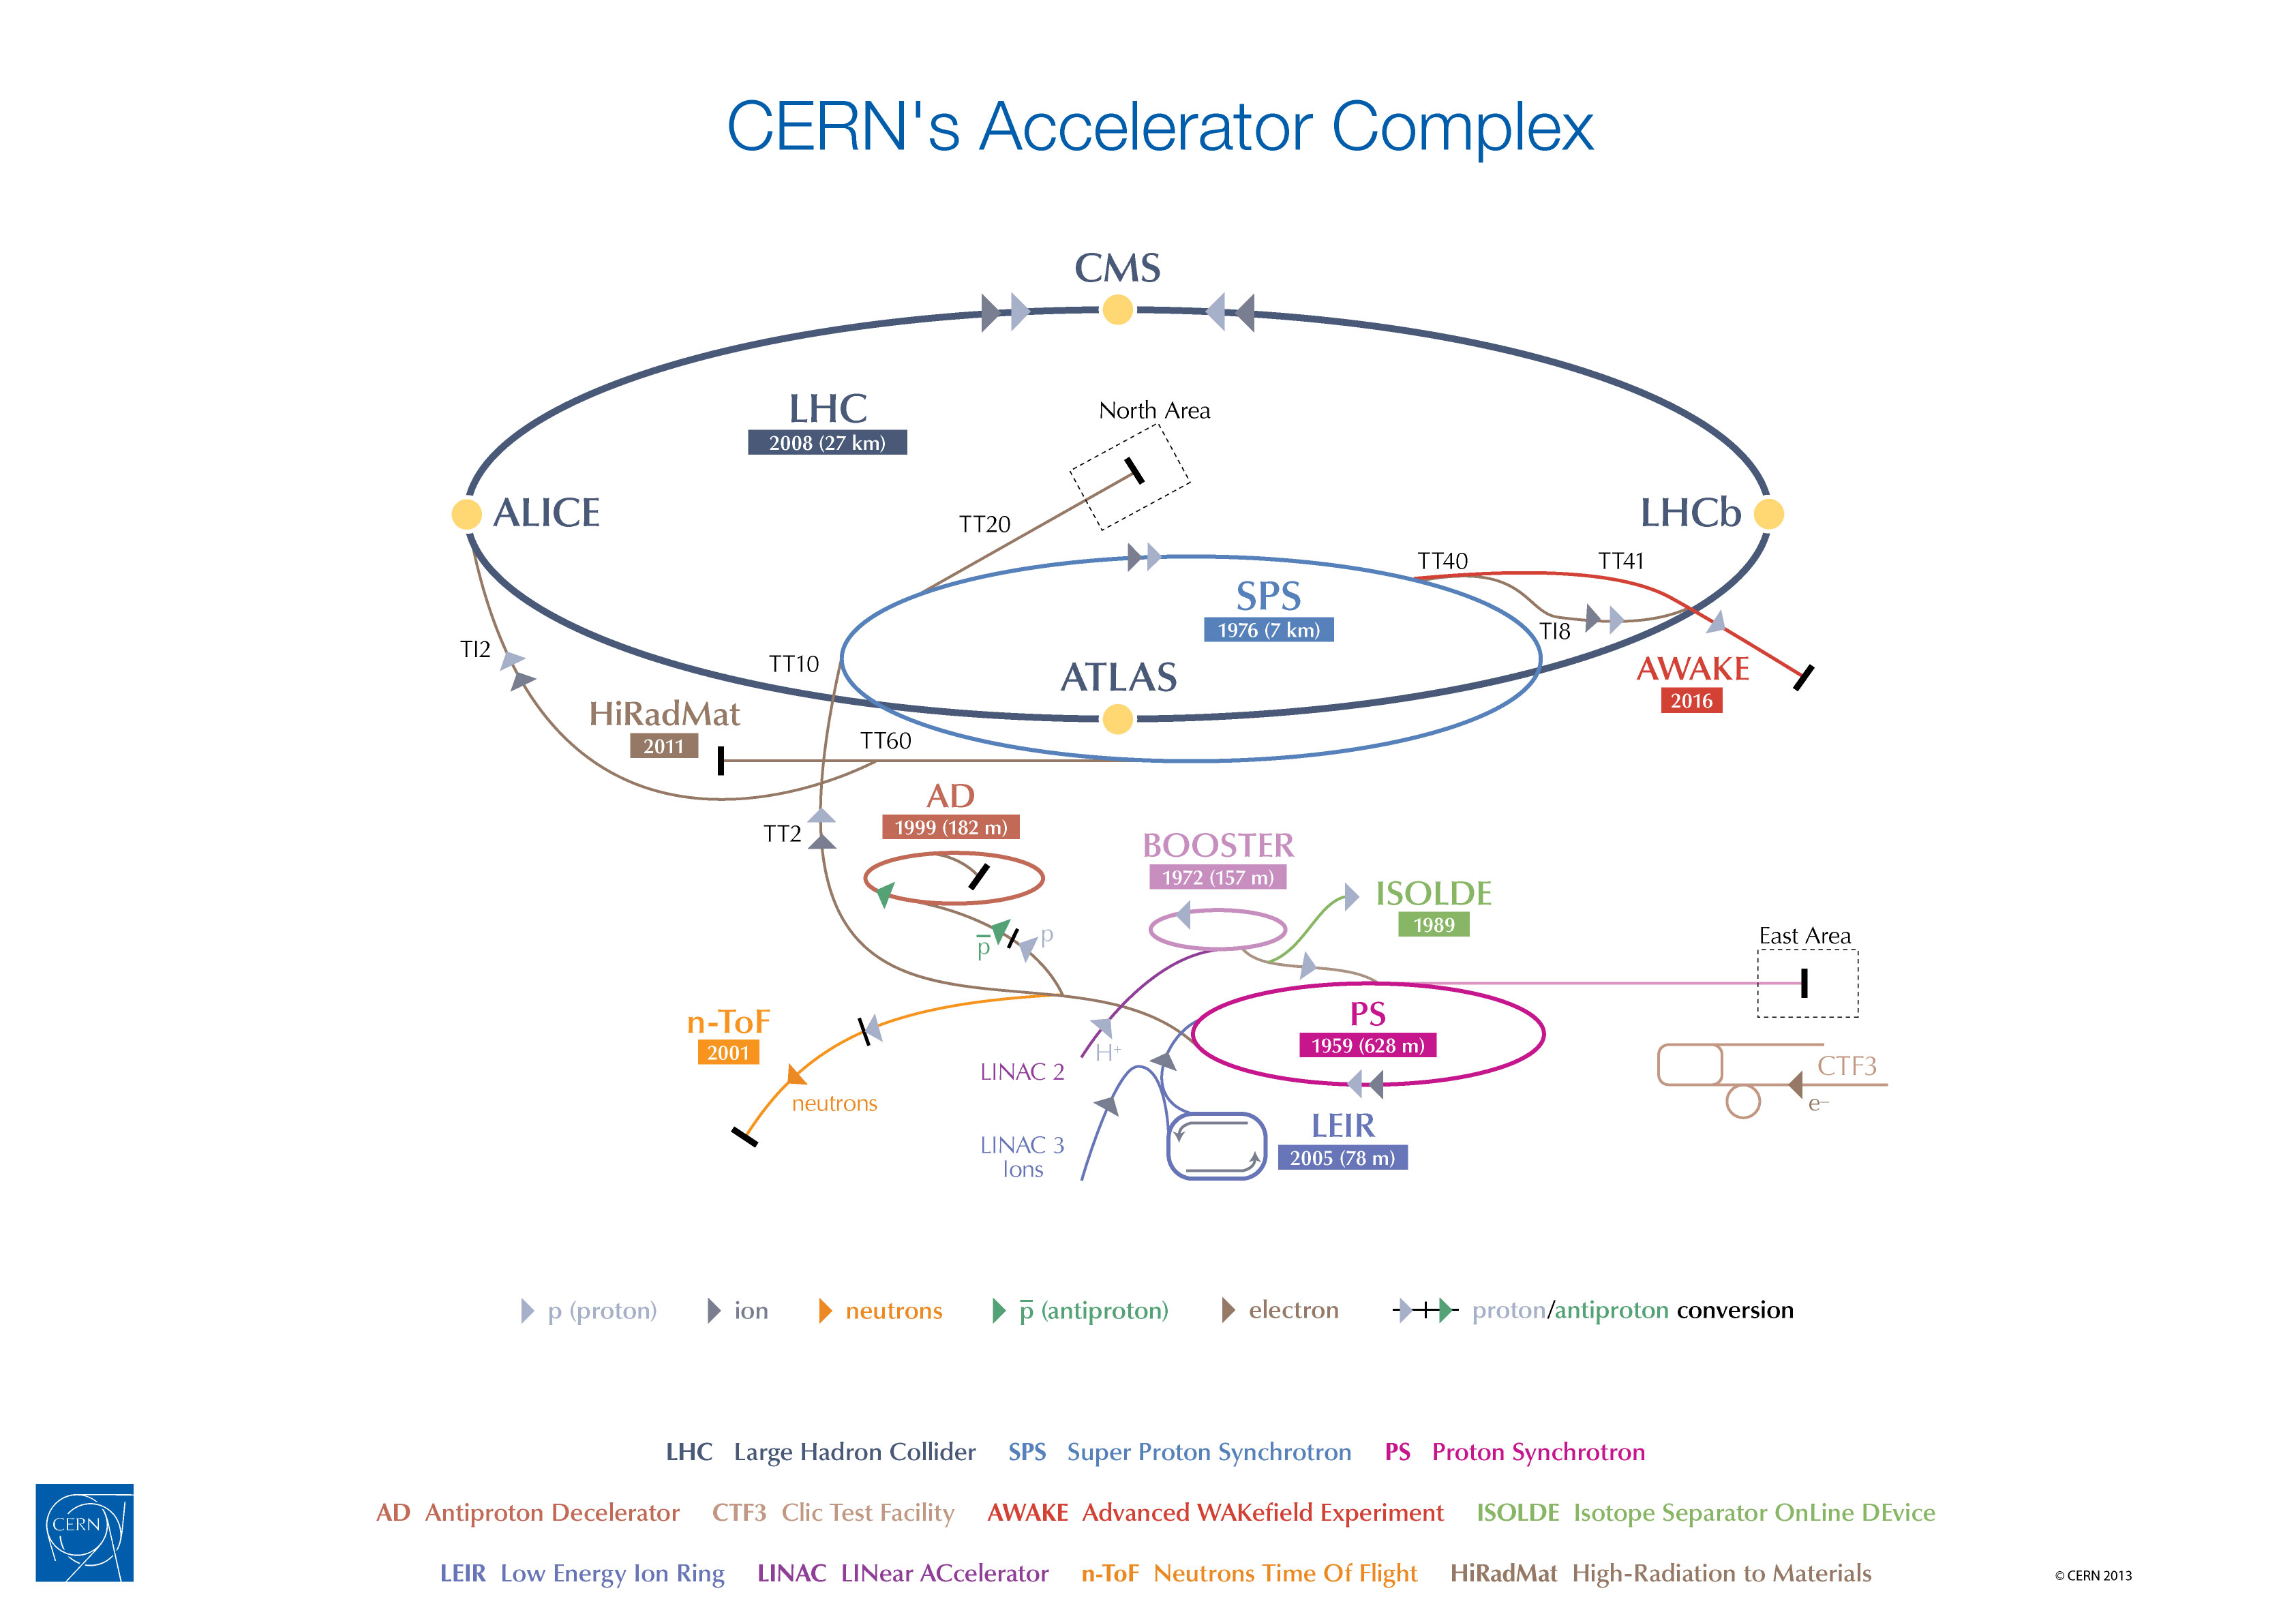
\includegraphics[width=\columnwidth]{gfx/ch1/CERN's-accelerator-complex2013.jpg}
    \caption[The LHC]{The LHC along with its accelerator complex.}
    \label{fig:cernacc}
\end{figure}

Protons are accelerated and injected in the LHC by a chain of four accelerators.
The first one is a linear accelerator that injects particles in a chain of three circular
accelerators. Finally, they are injected in the LHC with opposite directions in
two separate beam pipes with an energy of 450 GeV. The particles are accelerated
inside LHC by \emph{radio-frequency cavities} from 450 GeV to a desing-energy of 7 TeV, therefore
the center of mass energy of particles collision is 14 TeV. They circulate
grouped in \emph{bunches}; each beam pipe contains about 2800 bunches in LHC and each
proton bunch has $\approx 10^{11}$ protons. The bunches are spaced 25 ns in time in the nominal
design therefore collisions happen every 25 ns, for a final event rate of about 40 MHz.

\paragraph{Luminosity and pile-up}

The collision rate of an accelerator is measured by its \emph{luminosity}. It´s a measurement of the number of collisions that can be produced in a detector per cm$^{2}$ and per second. The bigger is the value of L, the bigger is the number of collisions; a key parameter in the design of an accelerator.
Semi-qualitatively, if we define N$^2 \approx (1.15*10^{11})^2$ as the square of the nummber of protons per bunch, $t$ = 25 ns as the time between bunches and $S_{eff} = 4\pi\sigma$ as the \emph{effective section of collision}, depending on the transversal size of the bunch at Interaction Point ($\sigma \approx 16 \; \mu$m), we obtain L as:

\[ L = \frac{N^2}{tS_{eff}} \approx 10^{34} \text{cm}^2 \text{s}^{-1}
\]

A related quantity is the \emph{integrated} luminosity, which is simply defined as the integral of the luminosity over time.

Searching rare events requires a large number of collisions; for this reason, the
beams are \emph{compressed} in the transverse plane just before entering in the experiments, in order to increase the luminosity of each bunch crossing. Rare events searches need high luminosity, but at high luminosity the rate
of minimum bias collisions exceeds the
bunch crossing rate and there is more
than one minimum bias interaction per
bunch crossing. This effect is known
as \emph{pile-up}. Pile-up interactions produce noise and tracks that make object
reconstruction more difficult, therefore
a compromise has to be found: the higher
the luminosity, the rarer the events that can
be searched, but simultaneously we also have a worse event reconstruction.

\paragraph{Reference frame}

%\begin{figure}
    %\centering
    %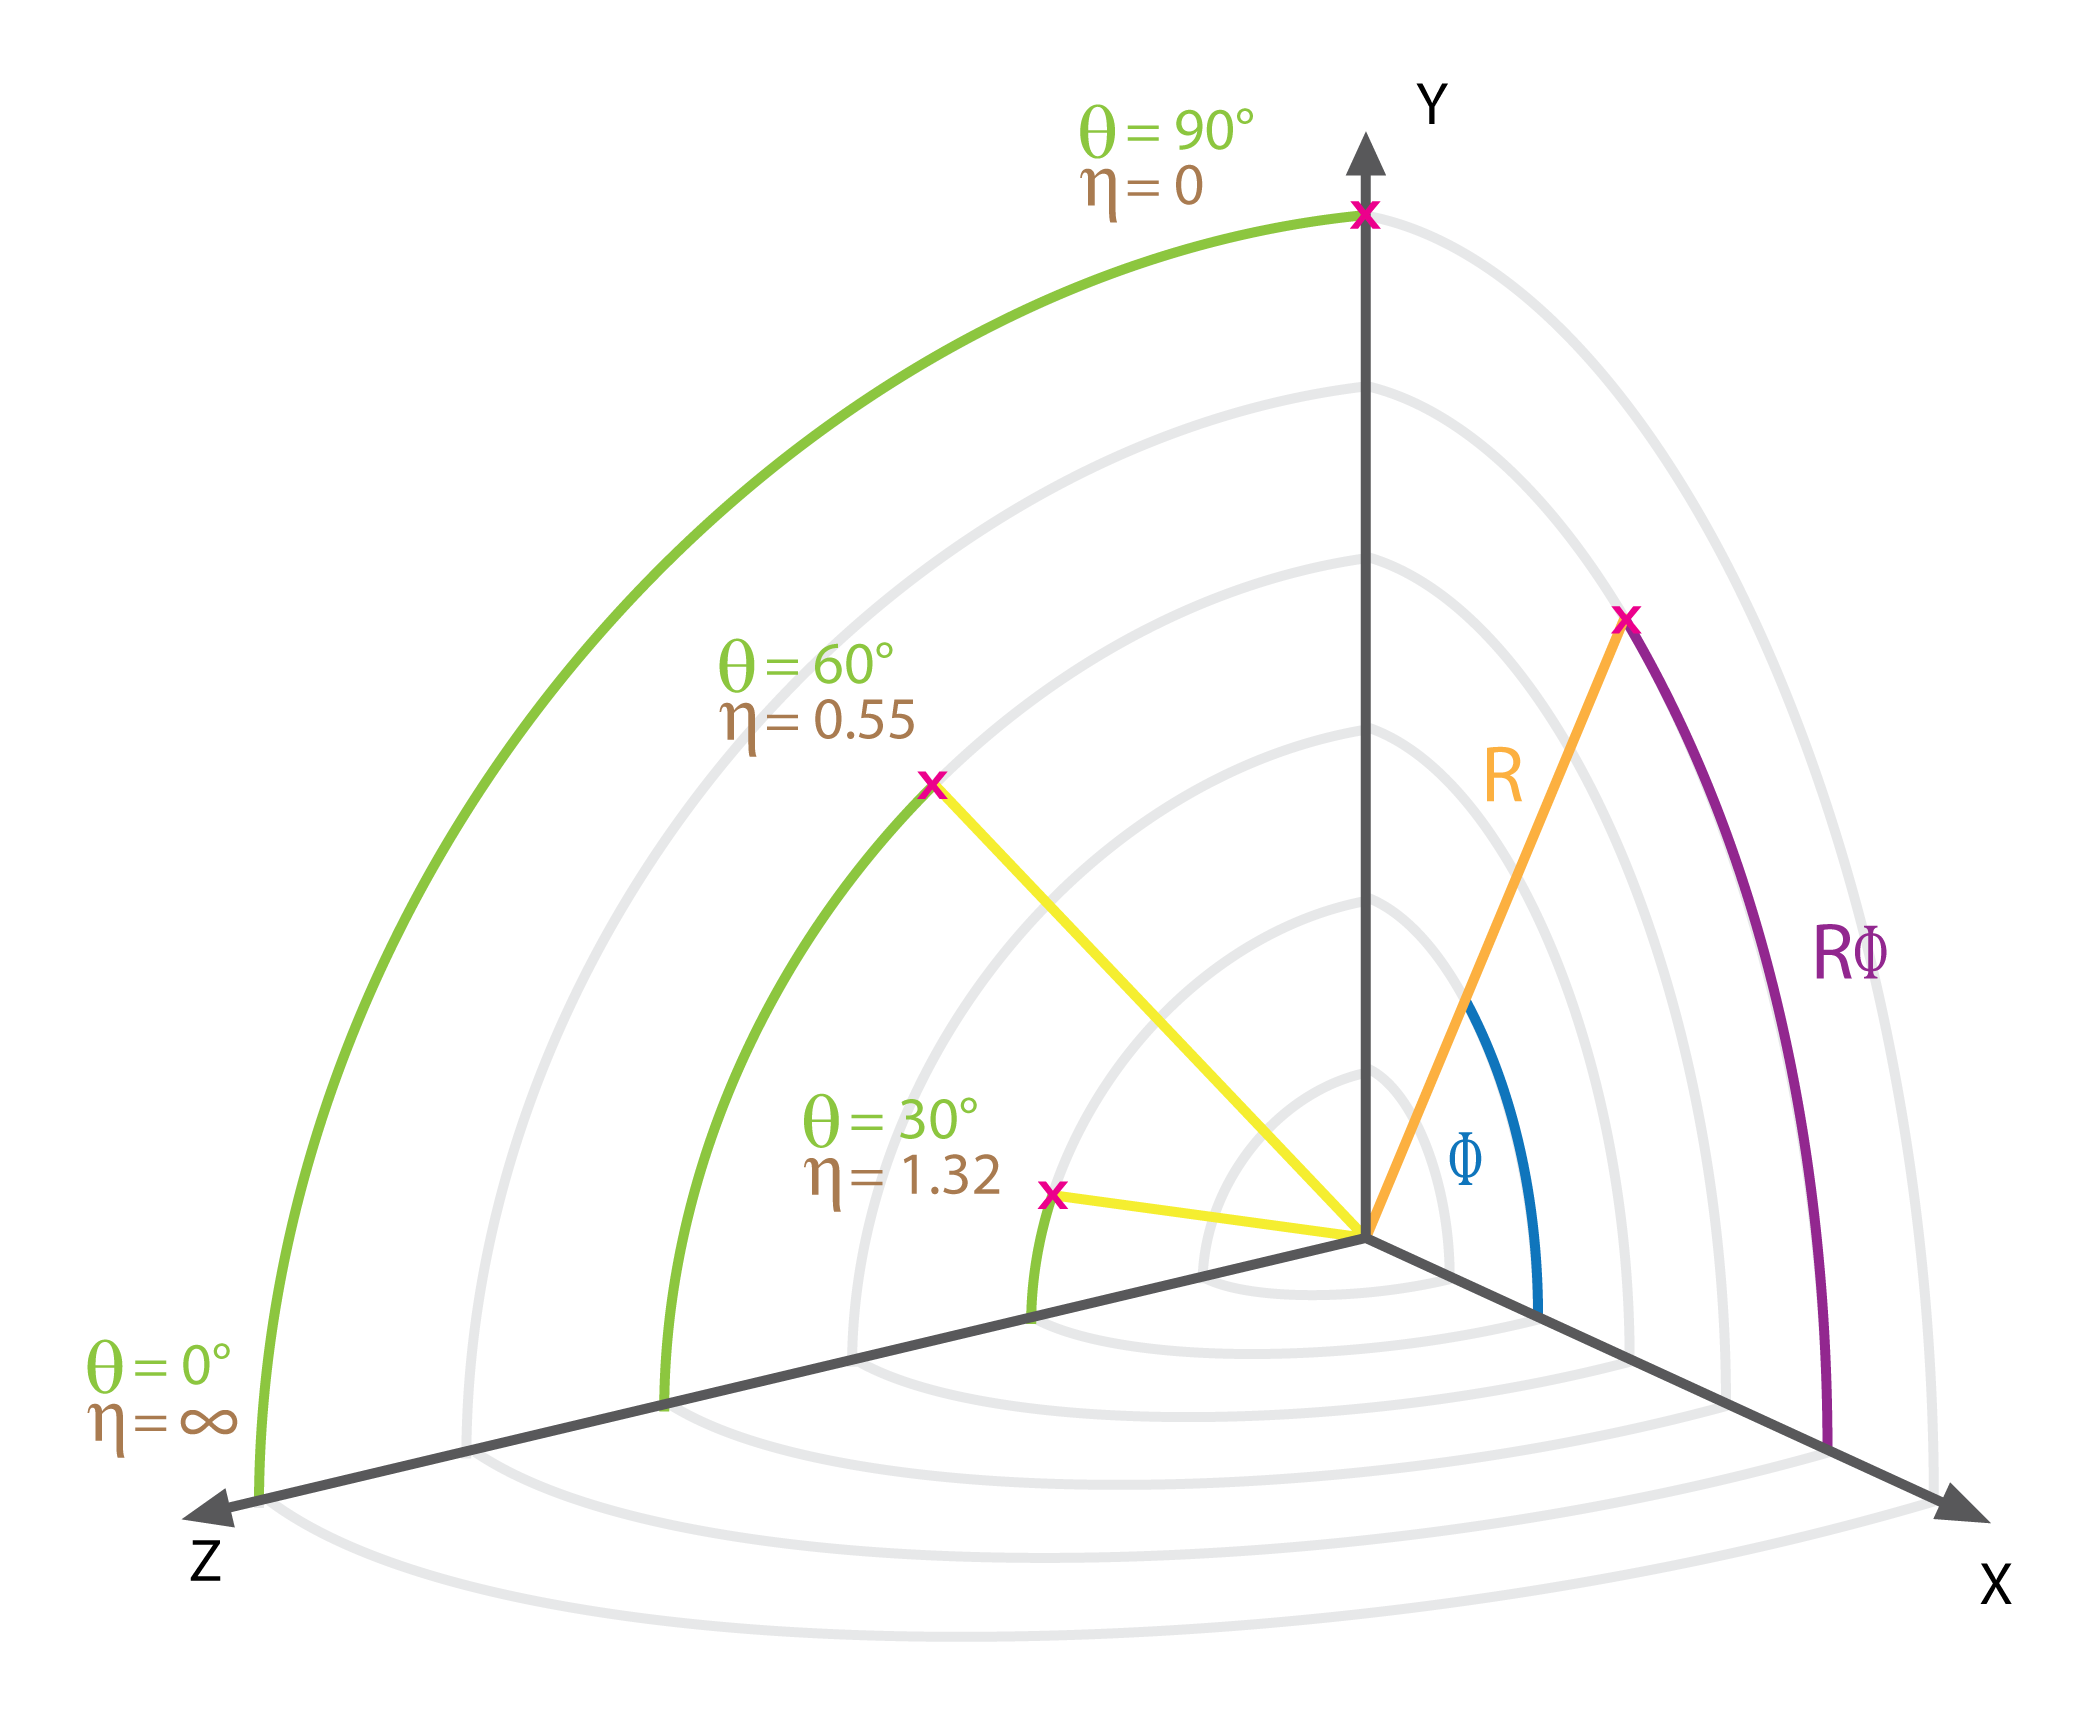
\includegraphics[width=\columnwidth]{gfx/ch1/img_cms_coordinates.png}
    %\caption[Reference frame]{The reference frame at LHC. The z-axis is pointing along the beam %direction. Taken from \cite{Lenzi:1551944}.}
%    \label{fig:reff}
%\end{figure}

The coordinate system used by the experiments at the LHC has its origin fixed at the nominal collision point. The x axis points towards the center of the LHC ring, the y axis points
upwards and the z axis points along the counter-clockwise beam direction. The \emph{azimuthal}
angle $\phi$ is measured from the positive x direction in the xy plane and the \emph{polar} angle $\theta$ is
measured from the positive z direction. The coordinate R usually indicates the distance from
the beam line (R $= \sqrt{x^2 + y^2}$)

In a typical collision, the center-of-mass of the interaction process is boosted along the
z axis with respect to the laboratory frame. The kinematics of the collision products are
therefore conveniently described by the coordinates ($p_T$ , $\eta$, $\phi$, $m$). Here, $\phi$ indicates the
azimuthal angle, $m$ the invariant particle mass and $p_T$ the transverse momentum given by $p_T =
p\sin\theta = \sqrt{p_x^2 + p_y^2}$. Letting $y$ denote the \emph{rapidity}, defined as:

\begin{equation*}
    y = \frac{1}{2}\ln(\frac{E + p_z}{E - p_z})
\end{equation*}

the transverse momentum, the azimuthal angle and the mass are invariant under boosts
along the z direction, while the rapidity is simply additive. The difference in rapidity between two particles is therefore invariant under boosts along the z direction.
The rapidity can however be approximated for ultra-relativistic particles by the \emph{pseudo-rapidity} $\eta$:

\begin{equation*}
    \eta = \frac{1}{2}\ln(\frac{\abs{p}+ p_z}{\abs{p} - p_z}) = -\ln(\tan\frac{\theta}{2}) 
\end{equation*}

which is computed using just the polar angle $\theta$ and is invariant under change of reference frame.

\section{The CMS Experiment}

The Compact Muon Solenoid (CMS) is a barrel shaped detector, centered at the
nominal point where the beams collide. It consists of a central part, called \emph{barrel},
and two external parts called \emph{endcaps}, placed at the ends of the cylindrical barrel.

CMS is a complex apparatus composed of many \emph{subdetectors}--it is illustrated in Figure \ref{fig:cms}.

\begin{figure}
    \centering
    \includegraphics[width=\columnwidth]{gfx/ch1/cms_160312_02.png}
    \caption[CMS]{The CMS experiment and its main components.}
    \label{fig:cms}
\end{figure}

The key feature of CMS is its superconducting solenoid that provides a magnetic field of
3.8 T with the axis aligned along the beams direction. The bore is 13 m long and
it has a radius of 3 m. The magnetic flux is returned by an iron yoke composed by
5 wheel in the barrel and three disk in each endcaps. The strong magnetic flux ensures enough bending power to measure the momentum of the highly energetic muons that
cross the detector.

Starting from the interaction point a particle crosses the\emph{ silicon tracker}, the \emph{electromagnetic calorimeter} (ECAL) and the \emph{hadron calorimeter} (HCAL) before reaching
the solenoid. Outside the coil the \emph{muon detection system} is inserted in the iron of the
yoke of the magnet.

\subsection{Design}

What follows is a brief description of the major subdetectors. As the technical details of each subdetector are extremely subtle, have already been studied and discussed in numerous articles and are not the focus of our study, we will not discuss them in the present work. The interested reader can found a detailed reference here \cite{Collaboration_2008}. Several upgrades have already been performed during the operational history of the detector, and more are to come in preparation for the \emph{High Luminosity} phase of the LHC.

\paragraph{Tracker}

The tracker constitutes the inner part of CMS and is designed to provide a precise
and efficient measurement of the charged particle \emph{tracks}, i.e. their curvature in the magnetic field, and of the primary and secondary
interaction vertices. It is immersed in an almost homogeneous magnetic field of 3.8 T provided by the CMS solenoid.

A \emph{silicon pixel detector} is installed in the inner region, closest to the interaction point, while \emph{silicon
microstrip detectors} are used in the outer region. The total length of the tracker is 5.8 m
and its diameter 2.5 m, and the angular coverage reaches up to $\abs{\eta}$ = 2.5. 

\paragraph{Calorimeters}

The calorimeters are located outside the tracker and inside the magnetic solenoid. They are
designed to measure the energy of electromagnetic and hadronic showers and, unlike the
tracker, they are required to completely absorb the particles in the shower for optimal energy measurements. They are therefore required to be \emph{heavy}, which translates into a large
number of radiation lengths $X_0$ for the ECAL and of interaction lengths $\lambda_I$ for the HCAL.
The full tracker material has a thickness of $\approx$ 0.5-1 $X_0$ and less than one $\lambda_I$ for comparison.

\begin{outline}
    \1 The ECAL is a homogeneous calorimeter made
    of 61200 PbWO4 crystals mounted in the central barrel part, completed by 7324 crystals in
    each endcap. The ECAL barrel covers the central rapidity region ($\abs{\eta}$ < 1.48) and the two
    ECAL endcaps extend the coverage up to $\abs{\eta}$ = 3. A lead/silicon-strip preshower detector is
    also installed at pseudorapidities 1.6 < $\abs{\eta}$ < 2.6. The crystals are all active material: they
    induce the shower and generate scintillation light to measure the shower energy. The scintillation light is detected by silicon avalanche photodiodes in the barrel region and vacuum
    phototriodes in the endcap region. 
    
    The typical \emph{energy reslution} is:
    
    \begin{equation*}
        \frac{\sigma_E}{E} = \frac{a}{E} + \frac{b}{\sqrt{E}} + c
        \end{equation*}
        
    where a $\approx$ 0.12 is the noise term due the electronics and pileup, independently of the energy, b $\approx$ 2.8$\%$ is
    the stochastic term which accounts mainly for the fluctuations in the photon conversions,
    and c $\approx$ 0.3$\%$ is a constant term related to the energy scale calibration.
    
    \1 The HCAL is used to measure the energy of hadrons, and it
    is the only detector available to measure the energy of stable neutral hadrons. Its design ensures
    good hermeticity to allow the measurement of the missing transverse energy and angular
    coverage in the forward region for forward jets.
    Four regions are instrumented with HCAL detectors: the barrel hadron calorimeter (HB)
    surrounds the electromagnetic calorimeter and covers the central pseudorapidity region up
    to $\abs{\eta}$ = 1.3; the two endcap hadron calorimeters (HE) cover up to $\abs{\eta}$ = 3. The Cherenkov-based, Hadronic-forward
    calorimeter (HF) extends the coverage up to $\abs{\eta}$ = 5 in the forward region. An array of scintillators, the outer hadron calorimeter (HO), is located outside the magnet to catch the tails
    of the hadronic shower and avoid the misidentification of muons. Contrary to ECAL, the HCAL is a sampling calorimeter: the energy is measured by scintillators alternated to brass plates used as absorbers in HB and HE.
    
    The HCAL is coarser than the ECAL and the resolution is also worse:
     the combined ECAL+HCAL resolution measured in a pion test
    beam was $\sigma_E /E = 110\%/\sqrt{E} + 9\%$.
\end{outline}

\paragraph{Muon chambers}

The muon system is located outside the solenoid and covers the pseudorapidity range
$\abs{\eta}$ < 2.4. Outside of the solenoid coil, the magnetic field flux is returned through a steel
yoke. Three steel layers are present both in the barrel and in the endcaps, alternated with
four layers of muon detectors.


The muon system provides information to identify muons and to measure the momentum
and charge of high-$p_T$ muons. Additionally, two tasks are accomplished by the muon system thanks to its good time resolution: \emph{bunch crossing} identification and \emph{muon-triggering}.
Three different gaseous detector technologies are used: \emph{drift tube} (DT) chambers and \emph{cathode strip} chambers (CSC), supplemented by a system of \emph{resistive plate} chambers (RPC). Both the DTs and the CSCs are primarily tracking detectors, but have also
good time resolution. The RPCs instead are mainly used for their good time resolution.


\paragraph{Trigger and Track reconstruction}

The 40 MHz rate of proton-proton collisions and the pileup make it impossible to process
and store all the information provided by the detector. Most of the events are not interesting
for physics analysis in any case, due the to fact that the total proton-proton cross section
is more than 6 orders of magnitude larger compared to the cross section of interesting processes. The data needs to be reduced and selected trough a trigger system, whose crucial
aspect is a fast and efficient real-time selection to record the useful events.

In CMS the data reduction happens in two steps. The \emph{Level-1} (or L1) Trigger consists of programmable electronic devices, reducing  the event rate from an input of 40 MHz to an output of about 100 kHz. The
\emph{High Level Trigger} (HLT) further decreases the event rate from about 100 kHz to about 1 kHz for data storage. The HLT is implemented by a computer farm composed of more than 30000 CPUs
running software modules similar to the ones used for the offline reconstruction. 

\paragraph{Offiline reconstruction}
Once the event has been selected by the trigger, other crucial, offline processing aspects are the \emph{track reconstruction}, the \emph{primary vertex reconstruction} and the \emph{particle flow} algorithm for particle identification. These are all needed to transform the electronic outputs of the apparatus into a collection of physical objects needed for the analysis.

\paragraph{Luminosity and Pile-up}

 The CMS designed luminosity of 10$^{34}$ cm$^{-2}$ s$^{-1}$ has been achieved and exceeded in the last three years of data taking. Integrated luminosity recorded by CMS and employable for physics analyses are 35.9 fb$^{-1}$ for 2016, 41.53 fb$^{-1}$ for 2017, and 60.0 fb$^{-1}$ for 2018.

As discussed above this also meant an increase in pile-up: Figure \ref{fig:pileup} shows its increase over the various years.

\begin{figure}
    \centering
     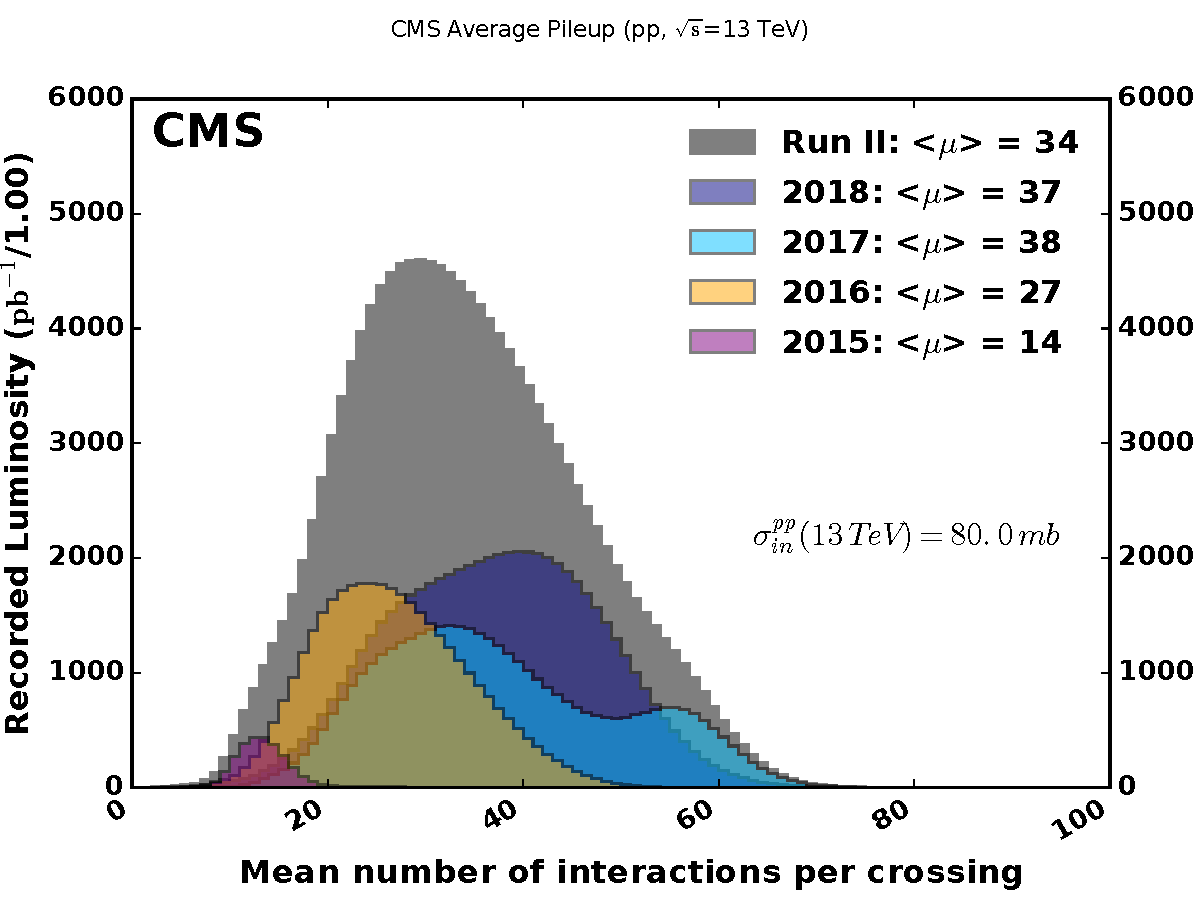
\includegraphics[width=\columnwidth]{gfx/ch1/pileup_allYears_run2.pdf}
    \caption[Pile-up]{The distribution of the average number of interactions per crossing (pile-up) for pp collisions in 2011 (red), 2012 (blue), 2015 (purple), 2016 (orange), 2017 (light blue), and 2018 (navy blue). From \cite{cmspubliclumi}.}
    \label{fig:pileup}
\end{figure}

\section{Physics program and measurements}

Being a general-purpose experiment, CMS is capable of performing a wide range of interesting and insightful measurements. Aside from the discovery of the Higgs boson and the study of its couplings, which will be discussed below in greater detail, we mention briefly the other directions of CMS research:

\begin{outline}
    \1 The \emph{SM physics} programme includes all the studies of the LHC data with the goals of measuring fundamental parameters of the Standard Model of particle physics. The cross-sections of a large variety of processes happening during the beam collisions are determined with the best precision possible and compared to the most up-to-date theory calculations, from the most common to the rarest of them all. Fundamental parameters of the theory such as masses of elementary particles and gauge couplings are measured to verify the effectiveness of the predictions, and any deviations of data from the Standard Model are quantified. The various \emph{couplings} expected between particles are investigated in detail. As an example, the \emph{Vector Boson Scattering} is a series of processes such as $W^{\pm} Z \rightarrow W^{\pm} Z$, however, it can admit higher-order couplings to the Higgs boson as $W^{\pm} Z \rightarrow H^{\pm} \rightarrow W^{\pm} Z$ which are to be investigated to compare their productions to what is expected from theory;
    
    \1 The \emph{Top Quark physics} programme consists in the precision measurements of the properties of the top quark, the heaviest particle in the standard model. The top-quark mass is one of the most important properties as it is a key parameter for calculations in the standard model. The top group also aims to establish measurements of rare production modes of the top quark in association with other particles, and search for new couplings of the top quark. It also aims to improve our understanding of top quark production and decay processes in order to improve background predictions as well as providing indirect proof for physics searches beyond the standard model;
    
    \1 \emph{Supersymmetry (SUSY), Exotica} and \emph{Beyond-Two-Generations} are a collection of groups working on generic processes beyond the SM predictions. SUSY consists in the search for physics signatures involving large missing transverse momentum, together with other features such as jets, muons, electrons, taus, photons, and b-jets. If we discover such signatures with yields significantly in excess of standard model backgrounds, our goal will be to characterize the event samples as fully as possible, as possible evidence of a supersymmetric theory. Exotica includes all the other processes not related to SUSY, while the B2G group covers models of new physics featuring the decay of new resonances to heavy standard model objects such as top, W, Z, or Higgs bosons. In particular, they study exotic \emph{diboson} resonances, partners of the top quark with vector-like properties (VLQ) as well as heavy resonances, such as W' and Z' resonances decaying to final states with top quarks.;
    
    \1 Fianlly, the \emph{B physics}groups addresses all the heavy flavor (beauty and charm) studies. These activities involve precision measurements of heavy-quark hadron production, decay and properties, and the search for associated new and rare processes;
    
\end{outline}

\subsection{The Higgs discovery and searches}

The main driver for the construction of the LHC and the deployment of the CMS experiment is certainly the Higgs boson and the detailed study of its properties. 

The Higgs is a \emph{scalar boson}, i.e. with spin $0$, whose presence in the theory is needed in order to explain the masses of the \emph{gauge bosons} (as well as the fundamental fermions) through the \emph{Higgs mechanisms}: a spontaneous symmetry breaking of the scalar fields embedded in the U(1)$\times$SU(2) local gauge symmetry of the electroweak sector. The mass of the Higgs particle is a \emph{free parameter} of the theory. The Higgs boson is also expected to  interact with the entire fermion sector trough \emph{Yukawa}-like vertices, with a coupling proportional to the fermion mass.

The Higgs boson, which is consistent with the SM Higgs according to the current experimental data, was discovered in 2012 at the LHC (see \cite{Aad_2012} and \cite{Chatrchyan_2012}). The mass of the new particle, approximately 125 GeV, sets the boundaries of today well-know Higgs phenomenology.

After having established the mass of the newly-observed boson, along with its major couplings during Run 1, both ATLAS and CMS renewed their efforts to improve the previous results and investigate the couplings of the Higgs to the fermions through Run 2 data. The most recent results published for the branching ratio signals are showed in Figure \ref{fig:sigsm}.

\begin{figure}
    \myfloatalign
    \subfloat[]
    {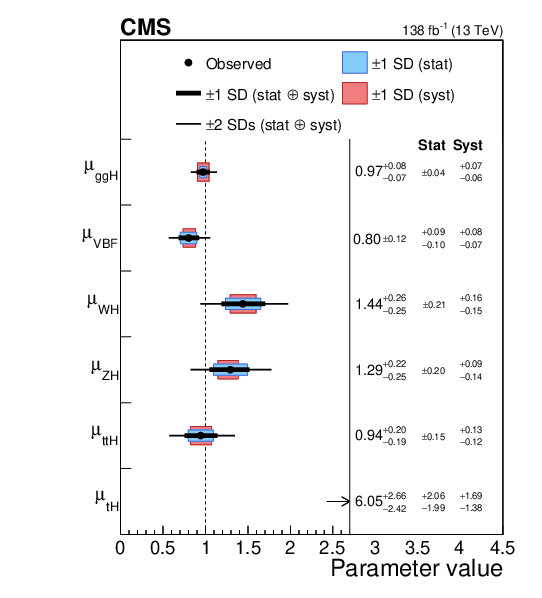
\includegraphics[width=.465\linewidth]{gfx/ch1/Figure_002-a.png}} \quad
    \subfloat[]
    { 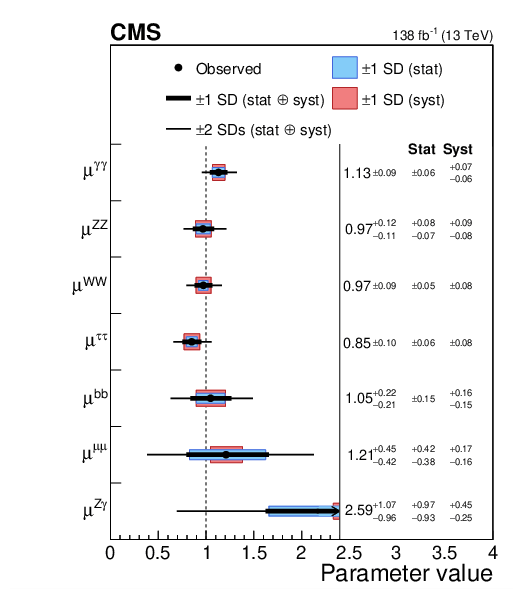
\includegraphics[width=.45\linewidth]{gfx/ch1/Figure_002-b.png}} \\
    \caption[Signal strength modifiers]{Summary plot showing the measured signal strength per
    production mode at $\sqrt{s}$ = 13 Tev (a) and the measured signal
    strength per decay channel at $\sqrt{s}$ = 13 Tev (b). Taken from \cite{higgsrevcms}}\label{fig:sigsm}
\end{figure}

They are expressed as the \emph{signal strength modifier} $\mu$, a ratio between the observed value and  the SM prediction, defined as:

\[
\mu_P = \frac{\sigma_i}{\sigma_{i, SM}} \quad \mu^D = \frac{\text{BR}_i}{\text{BR}_{i, SM}}
\]

where we have distinguished between the \emph{production} and \emph{decay} modifiers, and $\mu = \mu_P \cdot \mu^D$.

During Run 3, which is just starting at the time of writing, the
physics of the Higgs boson at the LHC is entering a time of precision measurements and
search for rare decays. Highly precise measurements are a powerful test for the theoretical predictions of the SM: small but significant deviations could appear which may hint at physics beyond our current theoretical description.

\subsection{The VBF Channel of H$\rightarrow\mu^+\mu^-$ as a benchmark for simulation}

\begin{figure}
    \myfloatalign
    \subfloat[]
    {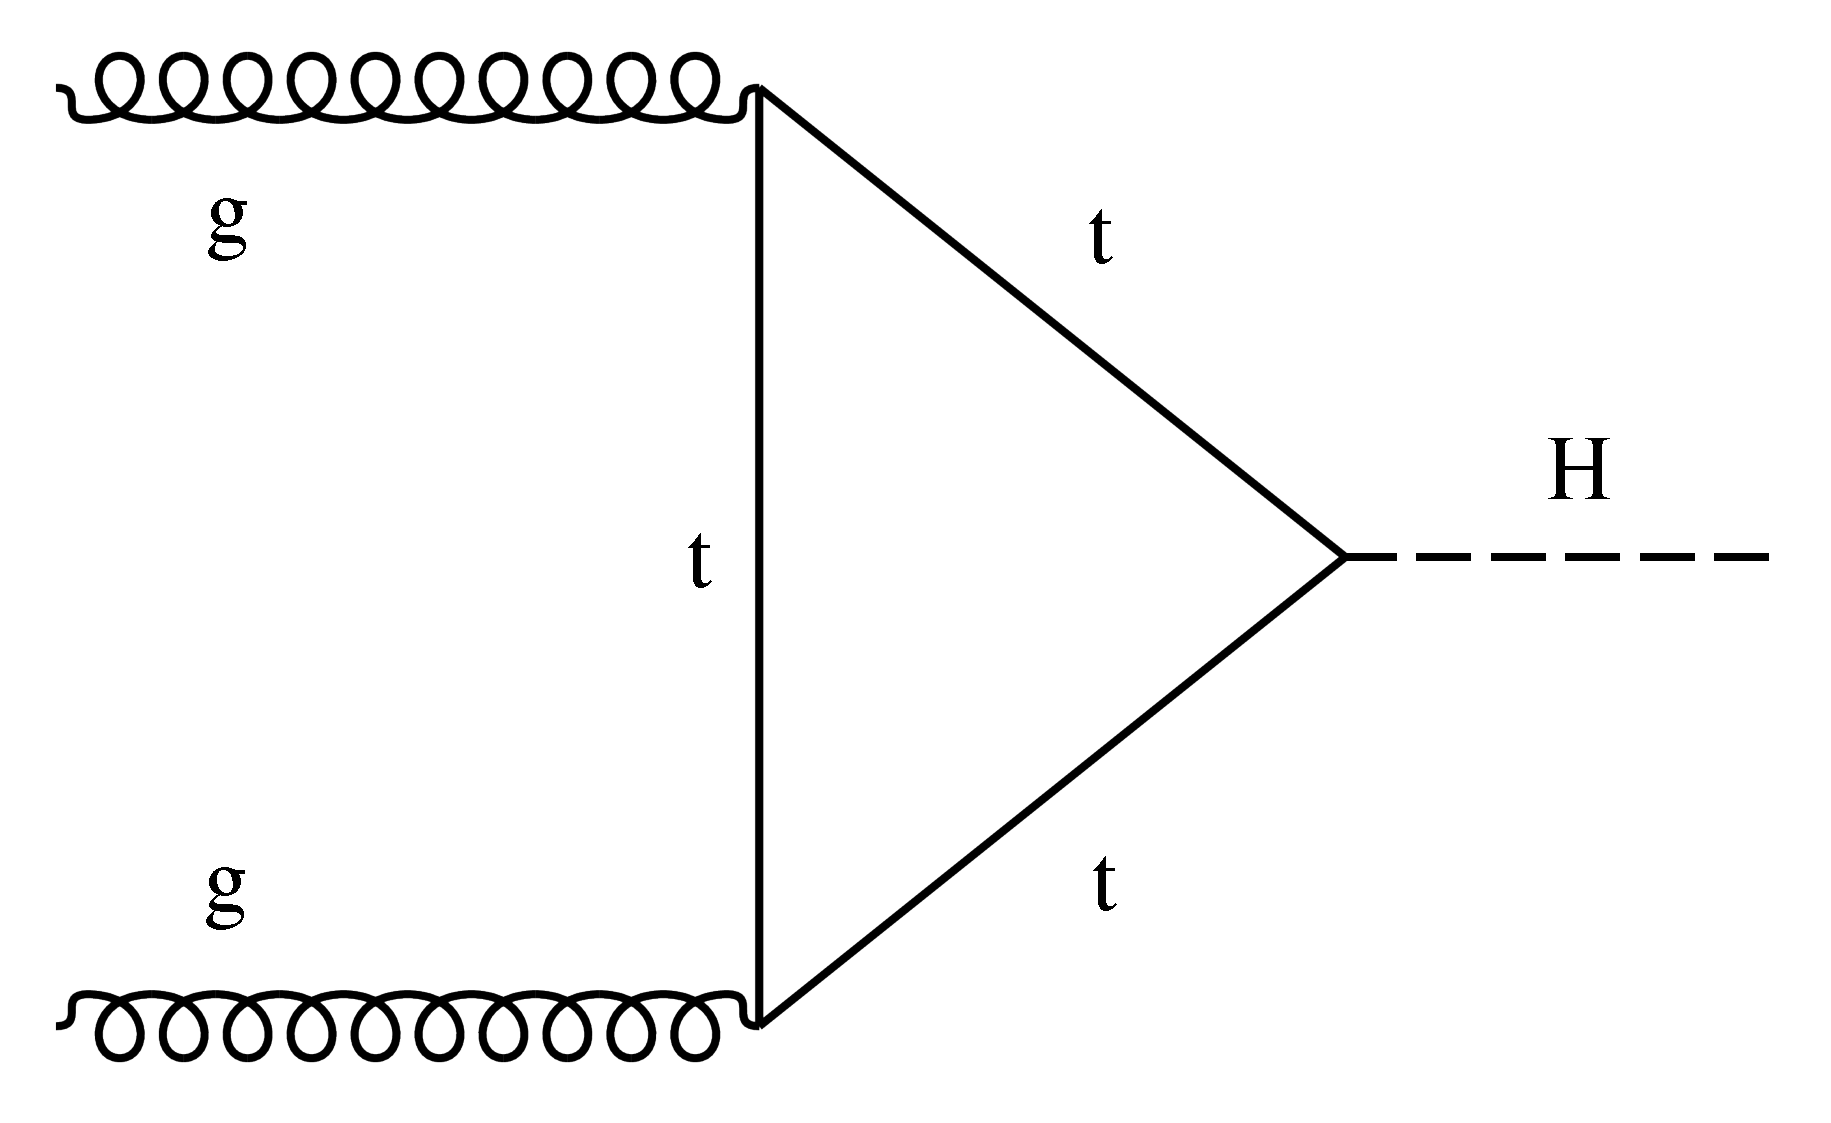
\includegraphics[width=.45\linewidth]{gfx/ch1/CMS-HIG-17-031_Figure_002-a.pdf}} \quad
    \subfloat[]
    { 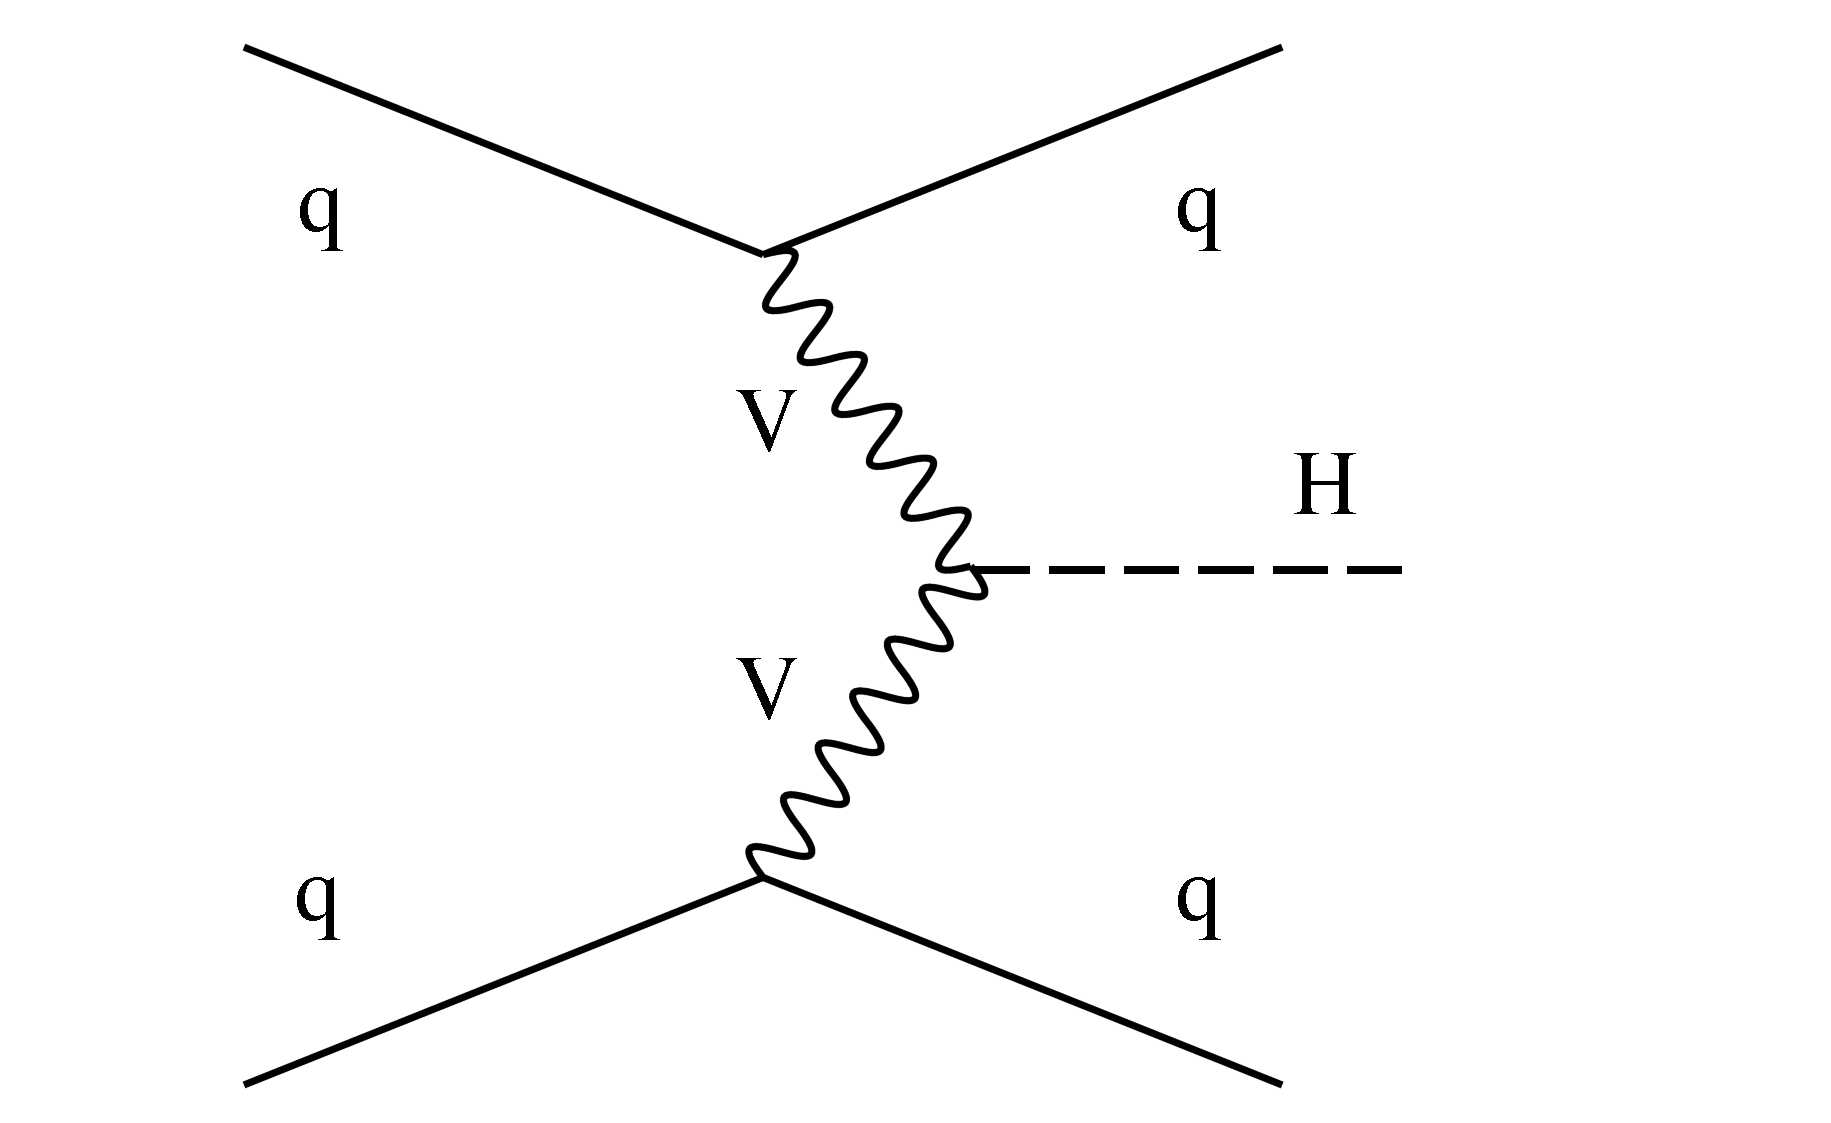
\includegraphics[width=.45\linewidth]{gfx/ch1/Figure_001-b.pdf}} \\
    \caption[ggF and VBF]{Leading Feynman diagrams for Higgs boson production via ggF (a) and VBF (b).}\label{fig:feypro}
\end{figure}
Having discussed the importance of the Higgs studies, we now present a specific production channel, as well as the two muon decay, explaining why they will serve as a solid benchmark for our deep learining approach to simulation.

In the SM, the phenomenology of the Higgs boson decays depends crucially on its mass,
which defines the branching fractions. The production modes instead have a milder Higgs
mass dependence. In proton-proton collisions at the center-of-mass energies currently reached by the LHC
(up to 13 TeV) four main production mechanisms are expected. The gluon-gluon fusion
production mode has the largest cross section, followed by vector boson fusion, associated
WH and ZH production, and production in association with a t$\overline{\text{t}}$  or b$\overline{\text{b}}$ pair. The gluon-gluon fusion (ggF) is the dominant production mode with a cross section of
approximately 85$\%$ of the total. The leading diagram involves a quark loop, given the fact that the H does not directly couple with massless gluons: the main
contribution to the SM amplitude arises from the top quark loop, though the amplitude is
potentially sensitive to the presence of new massive particles with non zero color charge.

The vector boson fusion (VBF) has a cross section of about a tenth of the gluon-gluon fusion one. The leading diagrams involve a qq scattering, with a
vector boson exchange and the emission of a Higgs boson. Since the momentum exchange
is typically lower than the center-of-mass energy of the two quarks, the channel is characterized by two separated high-rapidity quarks in the final state, detectable as high rapidity
jets. Their presence can therefore serve as a signature of the VBF production channel. Additionally, as VBF is a pure electroweak process, low hadronic activity is expected in the
rapidity gap between the two jets, where the Higgs decay products are typically found. The Feynman diagrams for the two dominant production processes are showed in Figure \ref{fig:feypro}. Experimentally, the signal over background ratio for the VBF channel is higher than that for other production modes, thanks to its key characteristics: few, energetic jets, highly energetic muons, a large rapidity gap.

This production mode is also an ideal candidate for our Flash Sim simulation approach, for a series of reasons:

\begin{itemize}
    \item The building blocks of the analysis are mainly the jets and the muons, meaning that we need to simulate a smaller number of physical objects when compared with other channels;
    \item The physical analysis is actually Monte Carlo-based, meaning that it is possible to validate our samples by comparing them to ones from the conventional simulation pipeline;
    \item A greater amount of MC-data would benefit the analysis by allowing a more accurate background modelling;
    \item Additionally, a flash simulation approach could also address the need for computing several different theoretical variations;
    \item More generally, due to the expected increase in luminosity during Run 3, the need for MC samples will also increase.
\end{itemize}

Additionally, the Pisa INFN Group worked extensively on the VBF Channel for the publication of \cite{CMS-PAS-HIG-19-006}, allowing us to take advantage of the expertise and insights of the group.
Because of this, in the latter part of this work we will compare the original samples employed in \cite{CMS-PAS-HIG-19-006} with the ones obtained through our approach.
At the time of writing, the CMS collaboration has managed to provide evidence of the H$\rightarrow\mu^+\mu^-$ up to 3$\sigma$ (see \cite{Sirunyan_2021}) Some relevant plots are shown in Figure \ref{fig:vbfmm}.

\begin{figure}
    \myfloatalign
    \subfloat[]
    {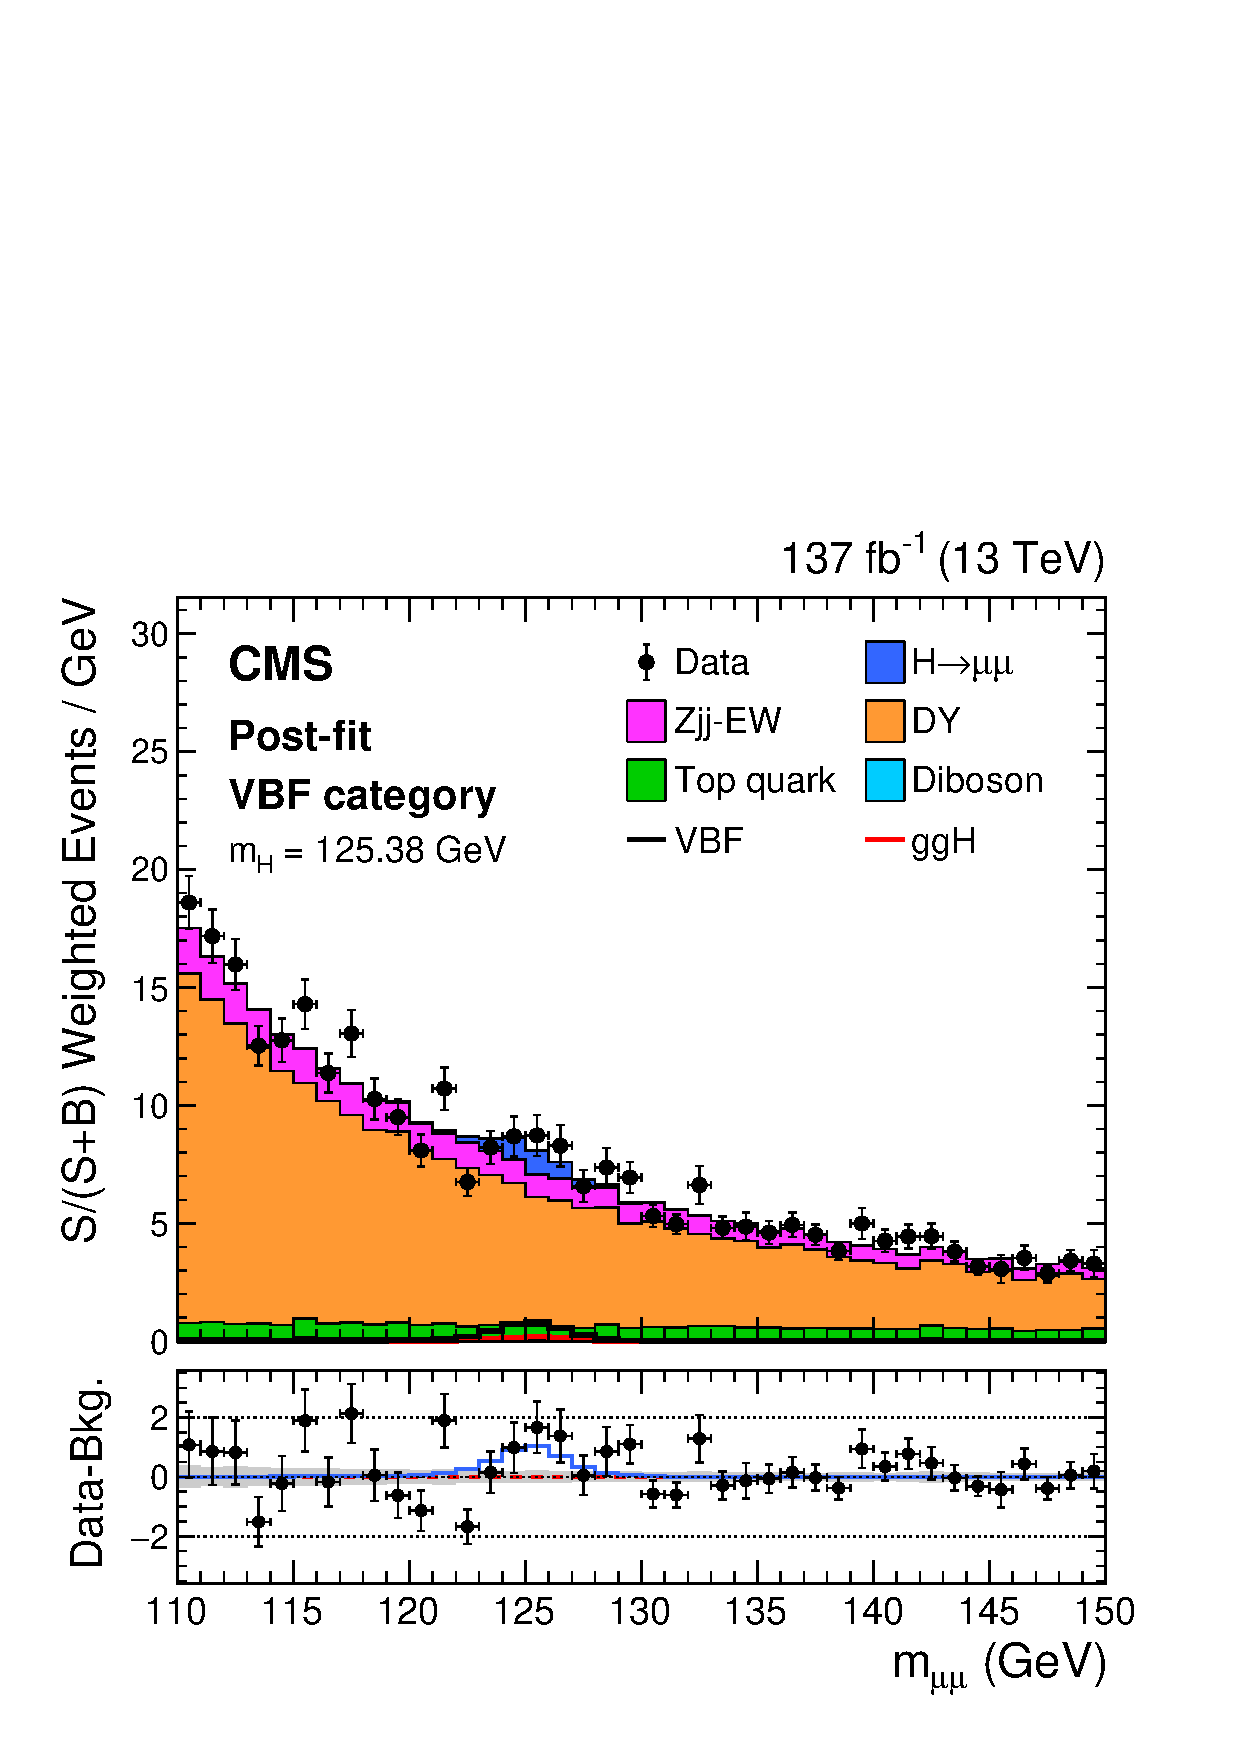
\includegraphics[width=.45\linewidth]{gfx/ch1/CMS-HIG-19-006_Figure_012-a.pdf}} \quad
    \subfloat[]
    { 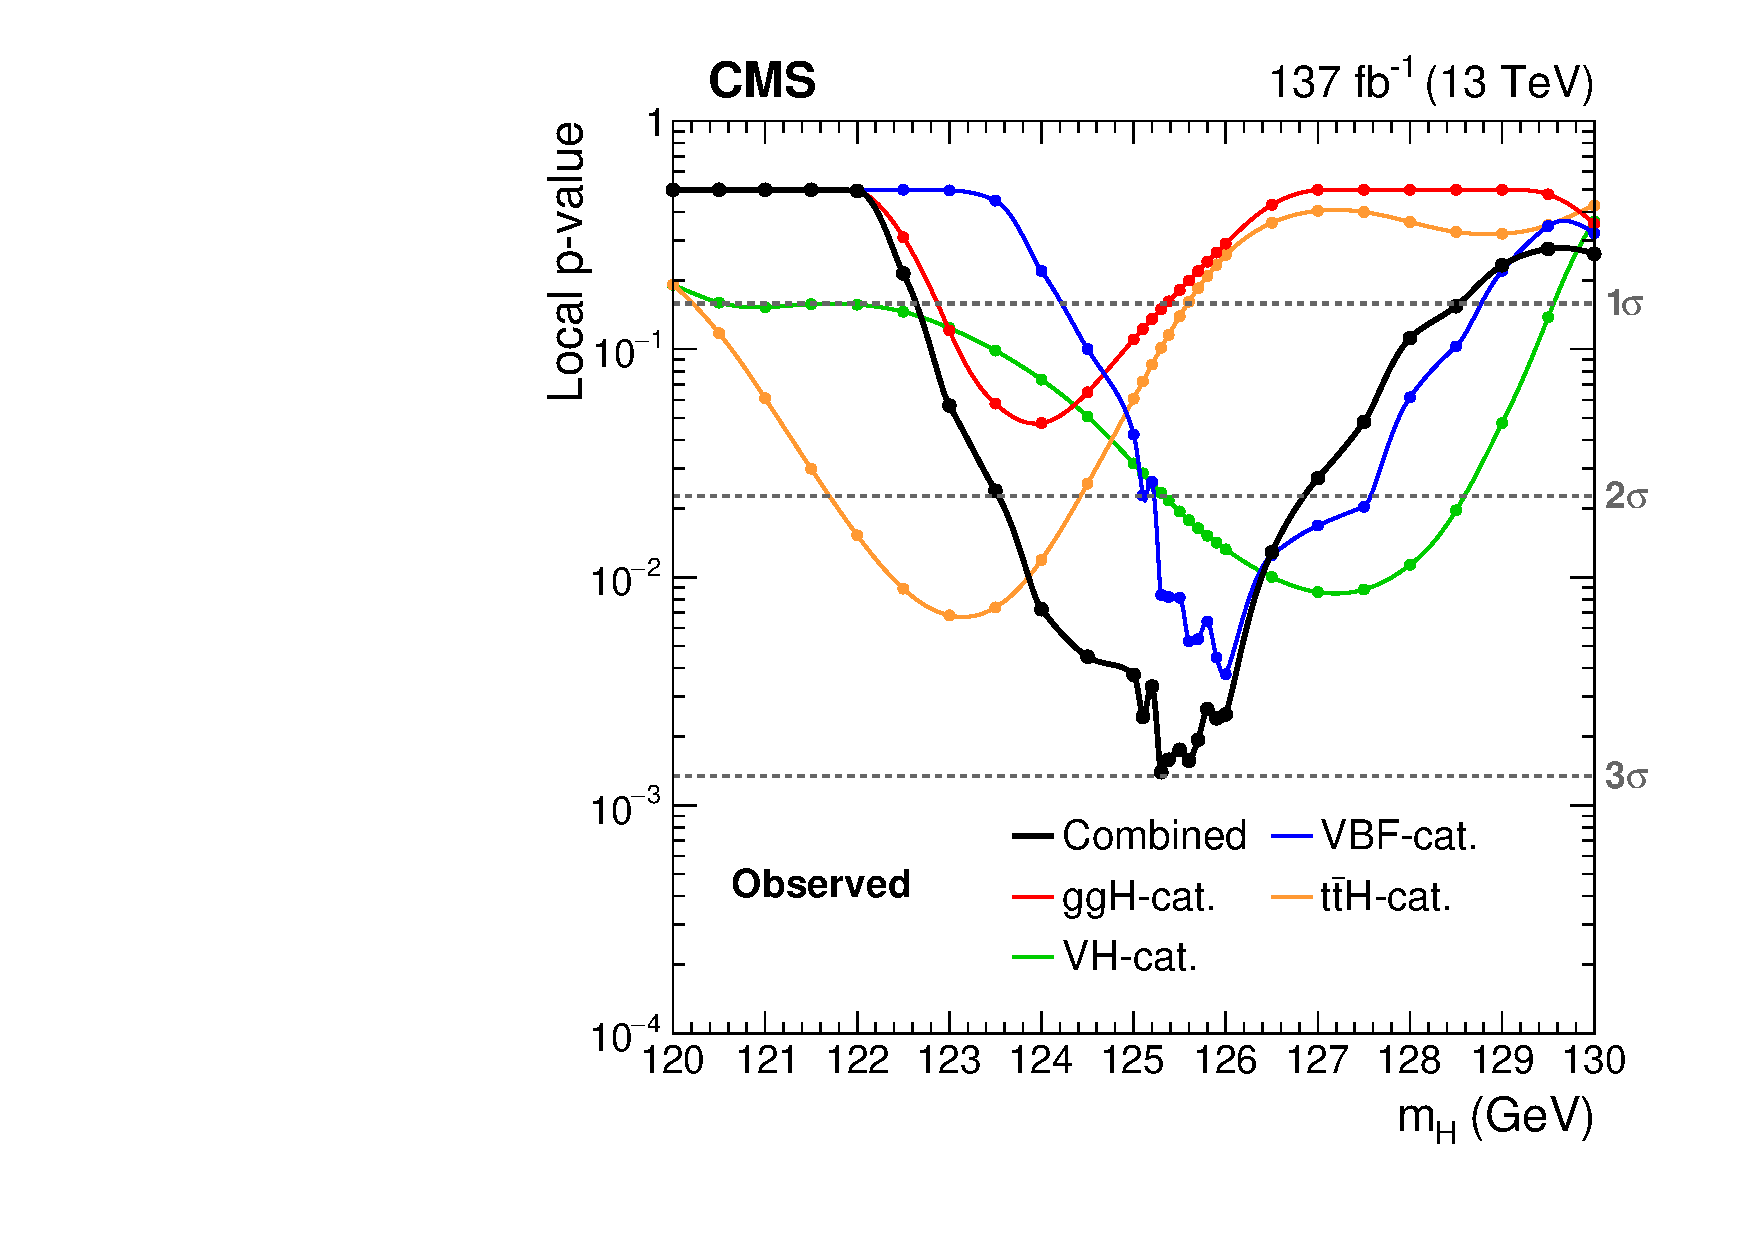
\includegraphics[width=.45\linewidth]{gfx/ch1/CMS-HIG-19-006_Figure_010-a.pdf}} \\
    \caption[H$\rightarrow\mu^+\mu^-$]{(a) The $m_{\mu\mu}$ distribution for the weighted combination of VBF-SB and VBF-SR events. The lower panel shows the residuals after subtracting the background prediction from the S+B fit. (b) Observed local p-values as a function of $m_H$, extracted from the combined fit as well as from each individual production category. It is clear that the VBF channel is the one providing the greatest evidence around the Higgs mass region. From \cite{Sirunyan_2021}.}\label{fig:vbfmm}
    
\end{figure}

Other possible processes which we could have chosen for comparison, and which would surely benefit from a flash production of samples, are the H$\rightarrow$bb decay as well as the ttH production mode. However, as we are presenting a \emph{proof-of-concept}, we decided to stick to the VBF channel as it present the unique advantage of needing simulations for just the jets and the muons, as opposed to the other candidates. 
%************************************************
\chapter{Data Analysis at the LHC}\label{ch:introduction}
%************************************************
The LHC produces -at design parameters- over 600 millions collisions ($\approx 10^9$ collisions) proton-proton per second in ATLAS or CMS detectors. The amount of data collected for each event, including pile-up, is around 1 MB (1 Megabyte). This means that we are reaching 40 TB/s of data--far too much for any detector data acquisition system to handle.

The trigger systems alleviate the problem by reducing the amount of data by a factor or 10$^{4}$; despite this, the constant need of cutting-edge resources and solutions, both in hardware and software, have been driving extremely fruitful research in the history of the LHC.

One major necessity, whose importance and scale may not be appreciated by people outside of the field, is the one for \emph{simulations}. We explain the concept more in detail in the following, drawing from \cite{sims} as an informal reference.

\section{The necessity of simulations}

First of all, we have to understand why do we need simulations in the first place.
The simulation is a crucial aspect of any high energy physics experiments. In CMS it is used both
at analysis level and for testing the algorithms before deployment with data. 
Simulations help in a wide range of scenarios:

\begin{outline}
   \1  The simulation can provide us with detailed studies of the expected SM background processes, allowing us to optimize our analysis according to the theoretical expectations;

\1 It can also target relatively rare processes originating from a hard interaction between twoproton components, which are signal or background for specific analyses. Single particles
or hadronic jets can also be simulated for specific purposes;

\1 Simulations are a necessity if testing possible extension of a physical theory, allowing us to understand what would we expect in this case. Then we can check which hypothesis our data looks like, and we can either validate or disprove the theory;

\1 Without a proper simulation, we also would not know the expected performance of the detector and the regions of interest for our process, making it impossible to properly operate the apparatus and obtain reasonable results.
\end{outline}
\section{Modelling an event} \label{sec:modelling}

There are three major, distinct steps in modelling a physical event at CMS. The first one,  \emph{generation}, is more generally related to the physical theories and calculations, while the other two, \emph{simulation} and \emph{digitization}, are specific to the CMS detector. The whole process is often referred to as \emph{FullSim} (full simulation).

\subsection{Event generation}

The first step to simulation is called generation, based on the theoretical calculations which describes how the quarks and gluons inside the protons scatter off one another, how they might create new particles, and how those new particles behave after they have been created. 

Proton-proton collisions are very complex and difficult to model accurately. Protons are
composed of 3 quarks, called \emph{valence} quarks, by virtual gluons and virtual quark anti-quark
pairs coming from gluon splitting. All constituents of hadrons are generically called \emph{partons}.
During high energy collisions, the protons behave as a collection of free partons and the
hard scattering can be described at the level of parton interactions. The hadronic cross
section $\sigma_{pp}$ is calculated based on the QCD \emph{factorization} theorem. The factorization theorem
states that the hadronic cross-section $\sigma_{pp}$ is a convolution of the partonic cross section  $\hat{\sigma}_{ij}$ with the parton distribution functions (PDFs) $f_i(x)$:

\[
\sigma_{pp} = \int_{x_{min}}^1 dx_1 dx_2 \sum_{i,j}f_i(x_1)f_j(x_2)\hat{\sigma}_{ij}(x_1 p_1, x_2 p_2)
\]

where function $f_i(x)$ is probability density that a parton of type i has a fraction x of the
hadron energy. The final cross section may be evaluated by the single, non-trivial contributions $\hat{\sigma}_{ij}$.

Apart from the hard interactions, i.e. parton-parton interactions with large momentum transfer which results into hard partons and jets, the other constituents of the proton can also interact. This
usually results in a spray of softer particles, called \emph{underlying event} (UE). Any high momentum particle involved in the collision will emit additional hard QCD radiation. Radiation
from particles before the hard interaction is called \emph{initial-state-radiation} (ISR), whereas radiation off particles produced in the collision is called \emph{final-state-radiation} (FSR). Quarks and gluons can emit additional radiation via the strong interaction. All the quarks
and gluons go through the hadronization process, forming colorless hadrons. Finally, unstable particles are going to decay. A representation of all these elements is shown in Figure \ref{fig:evgen}.          

\begin{figure}
    \centering
     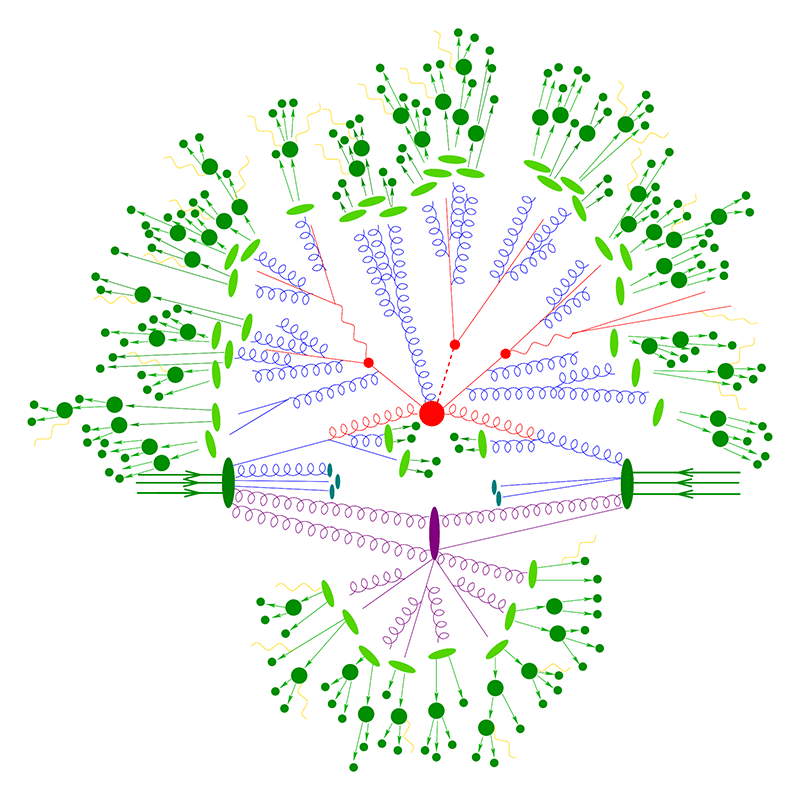
\includegraphics[width=.65\linewidth]{gfx/ch2/event_800px.png}
    \caption[Event generation]{ We can get a better understanding of a proton-proton collision event through this visualization. The red part includes the hard interaction and the decay of the products. Initial and final state radiation are in blue. A secondary
interaction can take place, in purple, before the final-state partons hadronize. The hadronization is
represented by the green blobs, and the hadron decay in dark green. Photon radiation is in yellow. From \cite{evgen}.}
    \label{fig:evgen}
\end{figure}


All the various parts involved in this step can be summarized as:

\begin{outline}
    \1  The PDFs that are phenomenological functions computed using experimental information;
    \1  the hard scattering, computed perturbatively order by order;
    \1  the parton \emph{showering}, used to simulate additional emissions in perturbative QCD;
    \1   the hadronization, describing the transition from colored particles to hadrons, treated
        using phenomenological models;
    \1   the decay of unstable particles, modeled based on experimental data.
    
\end{outline}

The first two are usually included in \emph{Matrix Elements generators}, while the last three are
included in Parton Showering programs. Both use Monte Carlo techniques; some popular multi-purpose generators include \texttt{Pythia8} \cite{Bierlich:2022pfr}, \texttt{MadGraph} \cite{Alwall_2014} and \texttt{Sherpa} \cite{Bothmann_2019}.

We can thus obtain a complete description of all the (stable) particles that come out of a collision between two protons under our theory only after a complex process involving several steps of modelling and calculations. The usual list of final state particles includes:


\subsection{Detector Simulation through GEANT4}

Now that we have the particles resulting from our process, we must take the detector into account. This means simulating all the interaction processes that are going to happen between particles and matter by moving them through the detector one by one and modelling the detector’s response to each one of the particles as it goes. 
Undoubtedly, the de-facto standard for such a task is the \texttt{Geant4} toolkit (see \cite{AGOSTINELLI2003250}). It is intended to simulate the passage of particles through matter and it includes a complete range of functionality including tracking, geometry, physics models and hits. The physics processes offered cover a comprehensive range, including magnetic field interactions, hadronic and optical processes, a large set of long-lived particles, materials and elements, over a wide energy range starting, in some cases, from 250 eV and extending in others to the TeV energy range. It has been designed and constructed to expose the physics models utilised, to handle complex geometries, and to enable its easy adaptation for optimal use in different sets of applications. The toolkit is the result of a worldwide collaboration of physicists and software engineers, created exploiting software engineering and object-oriented technology and implemented in the \texttt{C++} programming language.

\begin{figure}
    \centering
     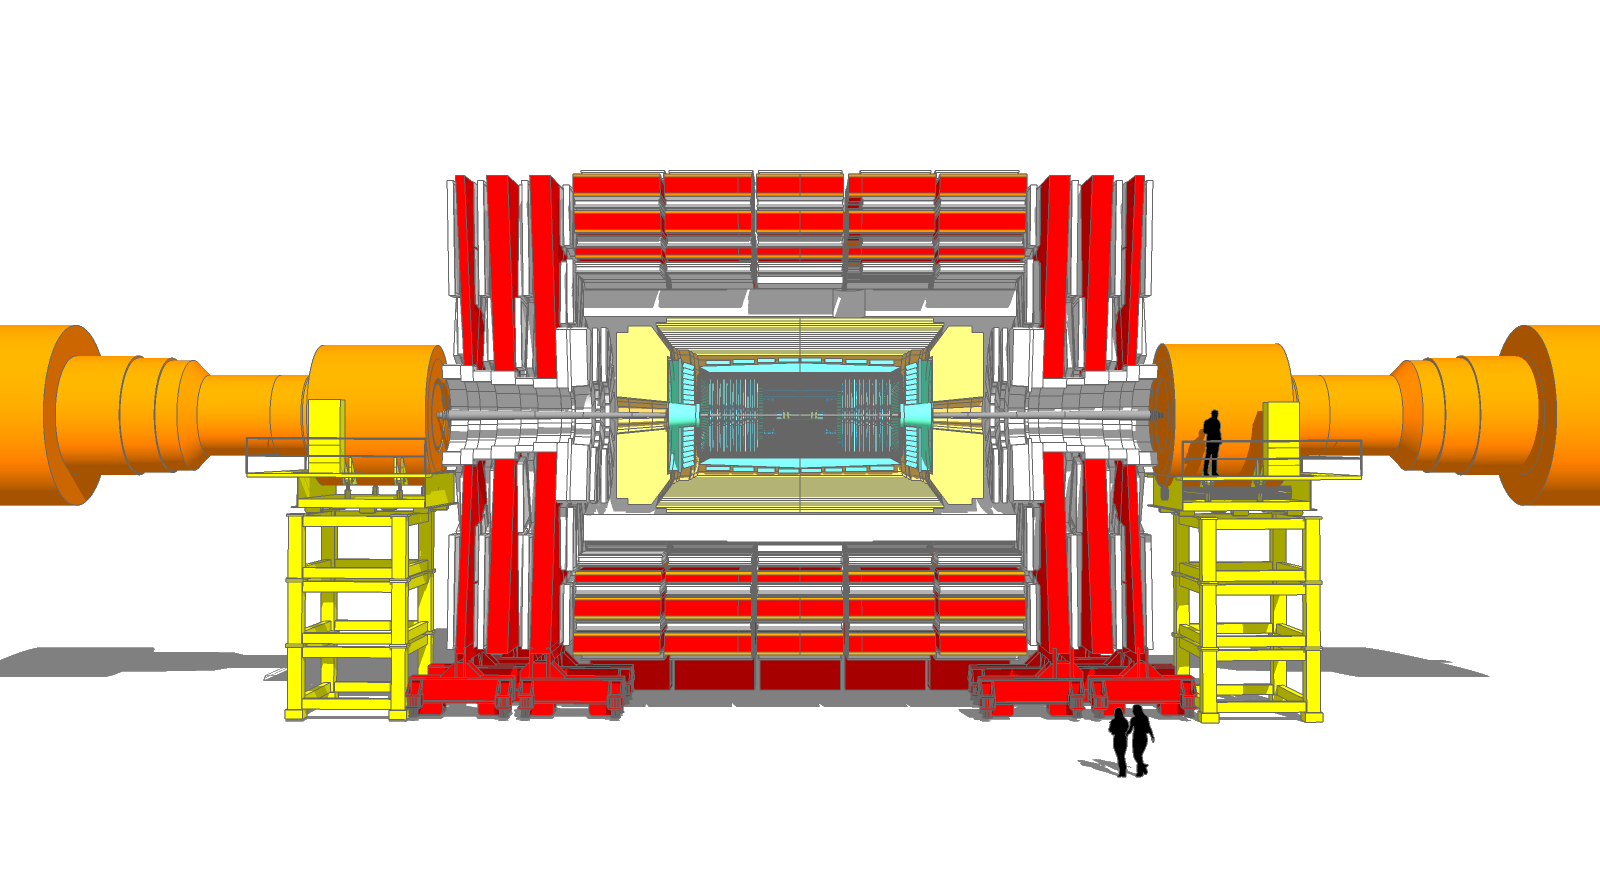
\includegraphics[width=\columnwidth]{gfx/ch2/cms_160518_01_Scene_2.png}
    \caption[CMS model]{ This representation of the CMS detector is based on the actual \texttt{Geant4} CMS Detector Description discussed in the text. It accurately and precisely reproduces the geometry of all CMS detector subsystems, including the geometries of the original CMS detector, phase 1 and phase 2 upgrades.  From \cite{decmod}.}
    \label{fig:decmod}
\end{figure}


However, \texttt{Geant4} can only provide us with a description of the single physical processes and materials, so we need to provide the actual \emph{detector description} (see Figure \ref{fig:decmod}). 

Every piece of the detector has to be put together, with the right material assigned to each. The full detector description has millions of volumes and hundreds of different materials.

Next comes the set of physics models. The toolkit has a great variety of them that can be used and they have a default quite suited to the HEP use case. Those physics models describe each process (e.g. the photoelectric effect, Compton scattering, bremsstrahlung, ionization, multiple scattering, decays, nuclear interactions, $\dots$) for each particle. Some calculations can be very complicated and costly, so we have to choose, at this point, what physics we are interested in. \texttt{Geant4} can be used for simulation of space, simulation of cells and DNA, and simulations of radioactive environments. It is usual to take the fastest model whose results we cannot really distinguish from the most detailed models. That is, we turn off everything that we don’t really notice in our detector anyway.

Finally, we specify the parts of the detector that are the most crucial, called \emph{sensitive} detectors. In the end we want to write files with all the energy deposits that  \texttt{Geant4} has made, their time and location – and sometimes information (called \emph{truth}) about what exactly happened in the simulation, so later we can find out how good our reconstruction software was at correctly identifying photons and their conversions into electron-positron pairs, for example.

At the end of this costly step, we are left with a long list of energy deposits, times, and locations in our detector. 

\subsection{Digitization and Reconstruction} 

The last part of the simulation process consists in turning the energy deposits into the actual signal outputted by the detector-- a process called digitization, once again specific for the CMS detector.

The simple idea is to change the energies into the detector outputs – usually times, voltages, and currents, for example. We have to build in all the detector effects that we care about. Some are well known such as Birks’ law, for example; others are more complicated, like the change in light collected from a scintillator tile in the calorimeter depending on whether the energy is deposited right in the middle or on the edge. We can use the digitization to model some of the very low-energy physics that we don’t want to have to simulate in detail with \texttt{Geant4} but want to approximate to an average. Those are effects like the spread and collection of charge in a silicon module or the drift of ionized gas towards a wire at low voltage.

Digitization is where some other effects are put in, like the pile-up, the extra proton-proton collisions in a single bunch crossing. We can add other background effects if we want to, like cosmic rays crossing the detector, or proton collisions with remnant gas particles floating around in the beampipe, or muons running down parallel to the beamline from protons that hit collimators upstream. 
At the end of the process we have something that looks exactly like the real data – except we know exactly what it is, without any ambiguity.

Finally, we also have to pass both our simulated data and the real data readouts to all the reconstruction algorithms of Section \ref{sec:offreco} to obtain a collection of physical objects as reconstructed by the detector readout. This is the \emph{reconstruction} step, resulting in events similar to the one shown in Figure \ref{fig:cmsev} . Detector hits after the simulation and reconstruction steps are called \emph{SimHits}
and \emph{RecHits} respectively.

\begin{figure}
    \centering
     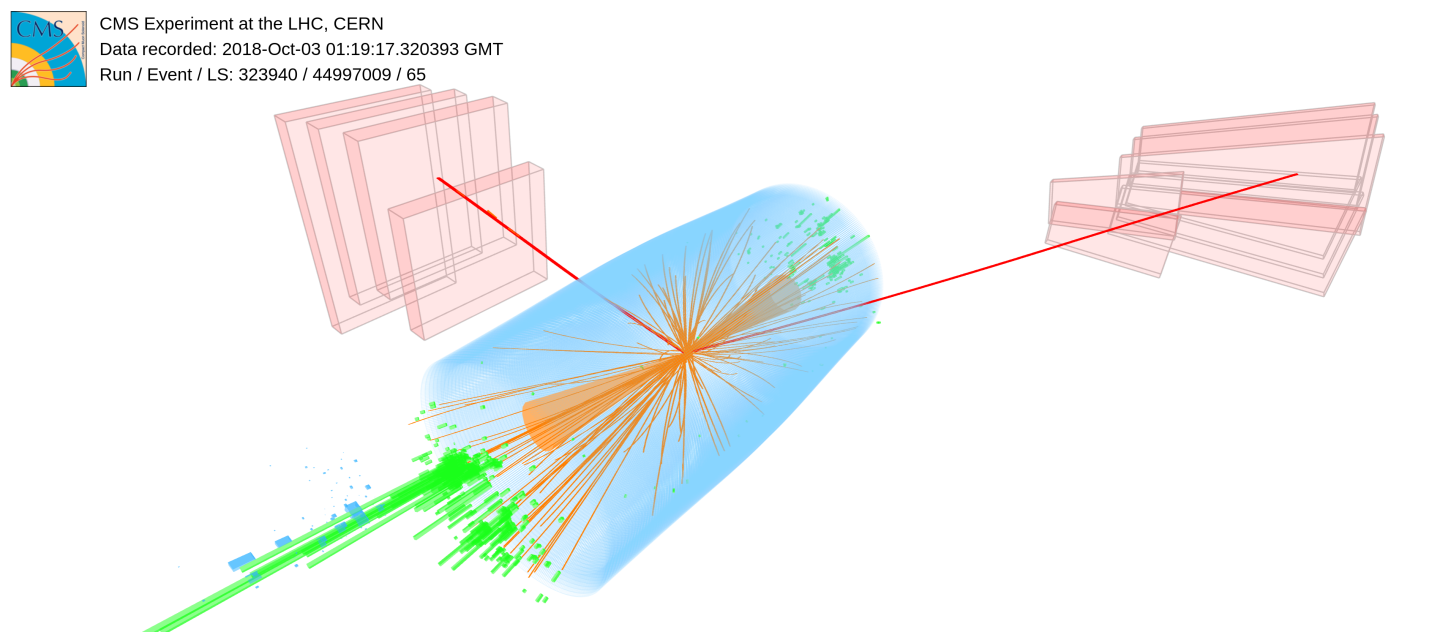
\includegraphics[width=\columnwidth]{gfx/ch2/HIG-19-006_VBF_white.png}
    \caption[CMS Event]{As an example of the final high-level event description, we show a final event description  where a candidate Higgs boson produced by vector boson fusion (VBF) decays into two muons, with an invariant mass of 125.01 GeV and per-event mass uncertainty of 1.83 GeV. The forward jets from the VBF are depicted by the orange cones and the muons are drawn as long red lines. Courtesy of the CMS Collection.}
    \label{fig:cmsev}
\end{figure}


Performing all the previous steps, we can build some simulated data that includes all sorts of different processes, like the production of top quarks, W bosons, Z bosons, and the Higgs bosons. And we can build another set that has all of those, but also includes other extensions of the theory. The last part, which is really what much of the data analysis is concerned with, is trying to figure out what makes events under the new hypothesis different from the other ones we expect to see – and trying to isolate them from the others. We can look at the reconstructed energy in the event, the number of particles we find, any oddities like heavy particles decaying away from the collision point – anything that helps. And we have to know potentially relevant information about the simulation, so that we do not end up using properties of the events that are very hard to simulate to separate new particles from known ones. 

Even if sometimes it can be useful to use \emph{data-driven} methods to estimate the backgrounds (or tweak the estimates from our simulation), it is common to start from the simulation itself to get a proper understanding of the expected background processes and their signals in the apparatus.

\subsection{Computing Costs}

Due to the length and the complexity of the process, its tremendous computation costs should not come as a surprise. Figure \ref{fig:cpuusage} shows the public approved HL-LHC CMS projections for the CPU usage at CMS.

\begin{figure}
    \myfloatalign
    \subfloat[]
    {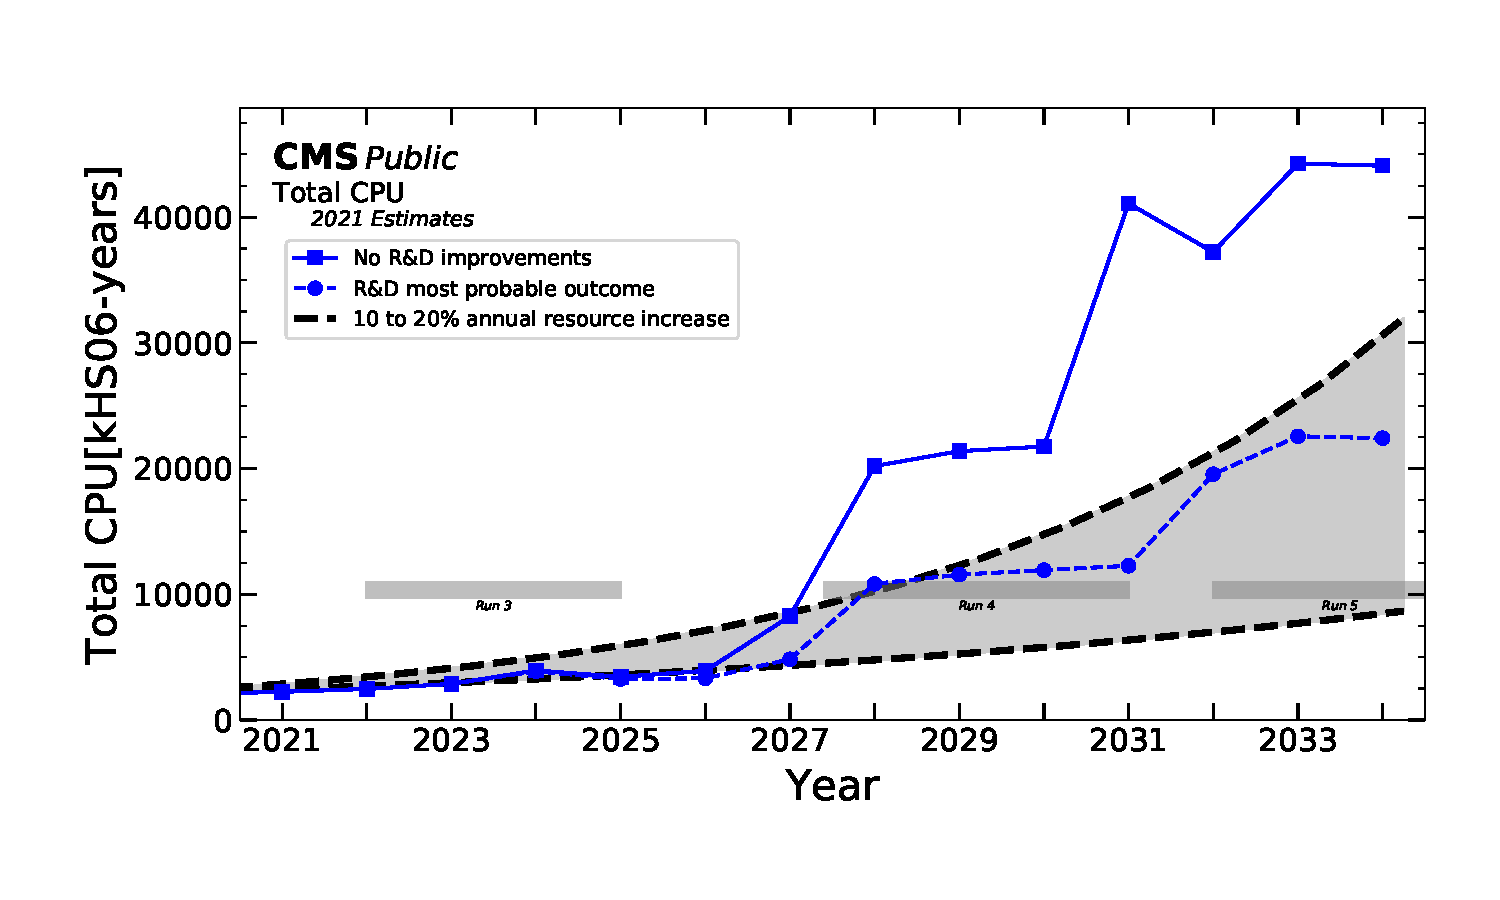
\includegraphics[width=.65\columnwidth]{gfx/ch2/cpu_cms2021.pdf}} \\
    \subfloat[]
    { 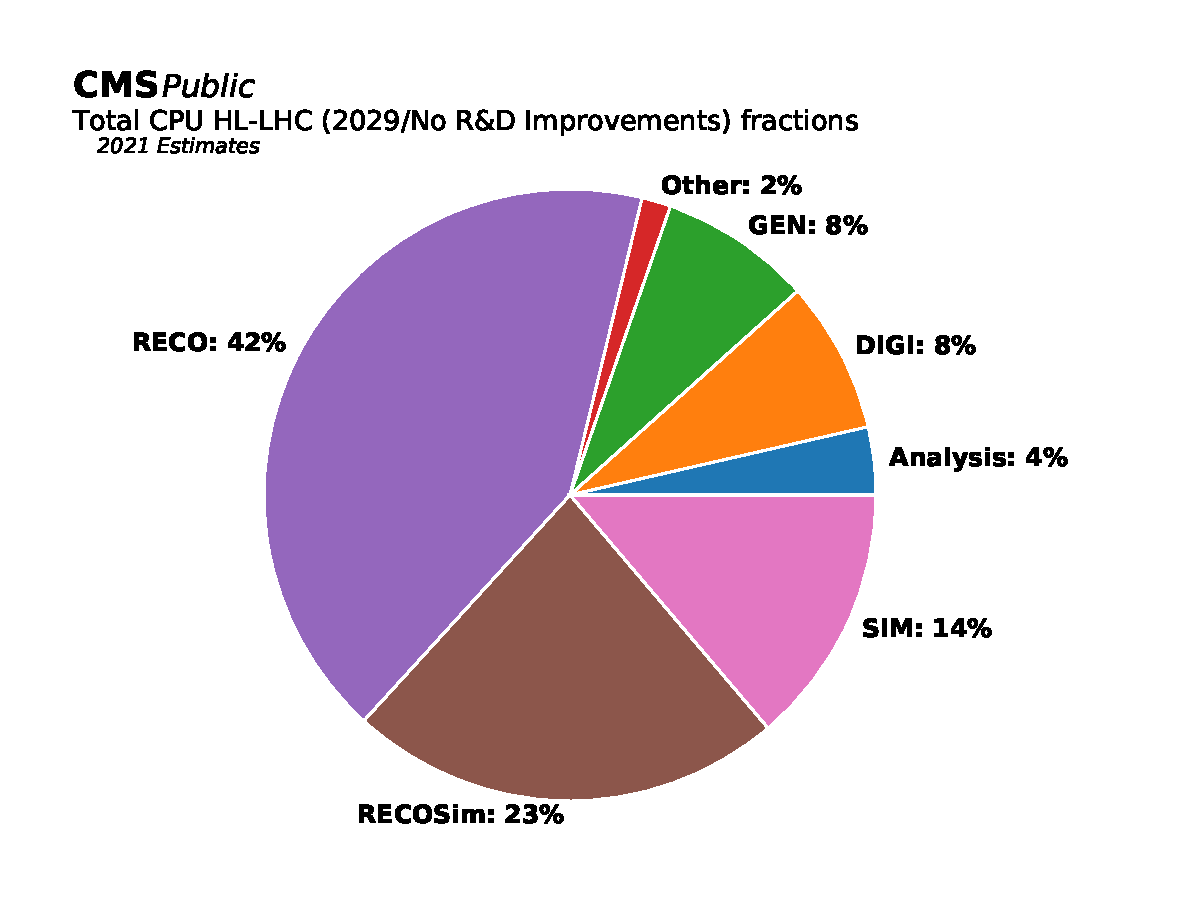
\includegraphics[width=.65\columnwidth]{gfx/ch2/cpu_pie_cms2021.pdf}} 
    \caption[Computing estimates]{The R$\&$D are necessary for the future of the experiment, as showed by the total CPU utilization projections (a) and the approximate breakdown of CPU time into primary processing and analysis activities (b) for the CMS experiment.}\label{fig:cpuusage}
\end{figure}

The plots show estimates from 2021 made for the CMS contribution to the LHCC November review of HL-LHC computing and common software, which supersede previous results from CMS. Coherently with the CMS Phase-2 Upgrade HLT TDR, an integrated luminosity of 270 fb$^{-1}$ per year at 140 pileup events (5 KHz high level trigger rate) and a 1.2 million seconds heavy-ions run is considered during Run 4. For what concerns Run 5, an integrated luminosity of 350 fb$^{-1}$ per year at 200 pileup events (7.5 KHz high level trigger rate) is considered during Run 5. Two scenarios are considered: the first one is a baseline, which does not include any improvement due to ongoing R\&D activity, and the second one incorporates the most probable outcome of the ongoing R\&D activities. The blue curves (and points) show the annual projected needs, summed across Tier-0, Tier-1 and Tier-2 resource needs in each of these scenarios. The gray band shows the projected resource availability for an example scenario that extrapolates the 2018 CMS pledged resources using an annual increase in available resources of between 10$\%$ and 20$\%$. Results are derived from a bottoms-up model of CMS offline processing activities, including prompt reconstruction, Monte Carlo simulation, data re-reconstruction and all phases of analysis activities. 

We also show the approximate breakdown of CPU time into primary processing and analysis activities during an hypothetical HL-LHC year. The plot corresponds to a snapshot of the year 2029. The baseline scenario is considered, i.e. projected effects from on-going R\&D that will reduce the computing resources needed by CMS are not considered.

The presented figures make it clear that:

\begin{outline}
    \1 Both the future and the present CPU (as well as Disk) utilization are completely dominated by the event simulation tasks, which leaves out about 48$\%$ of resources for other necessities;
    \1 Without improvements from the R\&D sector we risk not being able to meet the future necessities of the collaboration.
\end{outline}


\subsection{Fast simulation}

Clearly, the possibility of performing fast simulations would be a major improvement over the current simulation pipeline, and there are already many different studies and approaches for doing so.

\paragraph{Simplifying the interactions}

In this type of approach, we search for the slowest part of our process and find ways of making it as fast as possible with specific parametric shortcuts. The CMS Collaboration currently has a dedicated approach called CMS \emph{FastSim}, see \cite{https://doi.org/10.48550/arxiv.1701.03850}. 

While FullSim uses the exact detector geometry, tracks particles in small steps, and uses
detailed models for material interactions, FastSim uses a simplified geometry with simple analytical material interaction models that are parametrized
and tuned to agree with FullSim. For the digitization step, both FullSim and FastSim do a detailed
emulation of detector electronics and trigger, with small exceptions in FastSim. In the reconstruction step, FullSim employs the standard event reconstruction used for reconstructing the real CMS
data. FastSim uses standard reconstruction for calorimetry and muon systems, but a simplified
reconstruction for tracking, based on smearing and truth information, in order to reduce CPU time.

Performance of FastSim is validated regularly within the official CMS software release validation framework; overall, distributions in FastSim agree with FullSim within $\approx 10\%$ \cite{https://doi.org/10.48550/arxiv.1701.03850}. See Table \ref{tab:simfram} for a quick comparison with the others simulation approaches.

\paragraph{Starting from final-state objects}

The bottom-up approach means that we try to skip detector simulation and digitization all together and go directly to the final objects that we would have reconstructed (electrons, muons, jets, missing transverse momentum, $\dots$). A popular framework is the one of \texttt{DELPHES} fast-simulation, see \cite{de_Favereau_2014}.

It takes as input the final-state output of an event generator and performs a fast and realistic simulation of
a general purpose collider detector. To do so, long-lived particles emerging from the hard
scattering are propagated to the calorimeters within a uniform magnetic field parallel to
the beam direction. The particle energies are computed by smearing the initial long-lived
visible particles momenta according to the detector resolution. As a result, jets, missing
energy, isolated electrons, muons and photons, and taus can be reconstructed. It is oviously not meant to
be used for advanced detector studies, for which more accurate tools are needed, but it can nonetheless perform quickly realistic physics studies without in-depth knowledge of the technicalities. It should be noted that this type of strategy currently makes up the HL-LHC studies workhorse, as it is capable of providing acceptable results in a fraction of the time needed by the other approaches.


\begin{table}
\begin{adjustbox}{width={\textwidth},totalheight={\textheight},keepaspectratio}%
    \begin{tabular}{lll} \toprule
        \tableheadline{Simulation framework} & \tableheadline{key aspects} & \tableheadline{speed} \\ \midrule
        FullSim & \tabitem detailed geometry; &  $\mathcal{O}(40$ s) for a t$\overline{\text{t}}$ event \\
        & \tabitem small-step tracking; & \\
        & \tabitem \texttt{Geant4} material modelling; & \\
        & \tabitem  detailed digitization; & \\
        & \tabitem full reconstruction & \\
        \midrule
        FastSim & \tabitem simplified geometry; &  $\mathcal{O}(5$ s) for a t$\overline{\text{t}}$ event \\
        & \tabitem thin material layers; & \\
        & \tabitem simple analytical material modelling; & \\
        & \tabitem  detailed digitization; & \\
        & \tabitem full reconstruction with exceptions & \\
        %postulant quo & westeuropee & sanctificatec \\
        \midrule
        Delphes & \tabitem simple tracking system; &  $\mathcal{O}(0.01$ s) for a t$\overline{\text{t}}$ event \\
        & \tabitem smearing & \\
        %autem vulputate ex & parola & romanic \\
        %usu mucius iisque & studio & sanctificatef \\
        \bottomrule
    \end{tabular}
    \end{adjustbox}
    \caption[Simulation frameworks]{An at-glance comparison between the various simulation frameworks employed at the CMS experiment, useful for understanding the current approaches.}
    \label{tab:simfram}
\end{table}

As Table \ref{tab:simfram} shows, the various fast simulation approaches allow us to obtain significant speedups. However, while CMS FastSim accuracy is constantly being improved, its speed is still somewhat lacking; while \texttt{DELPHES} achieves a marked speedup but sacrifices the realistic detector simulation.

\section{The standard CMS Analysis format: NanoAOD}

Because the simulation consists of so many different steps, we end up with a large amount of information for each event. Aside from final state objects, we are able of keeping track of various steps as the particles pass through the detector, as well as individual components of jets, with great precision. Starting from raw data produced from the online system or the MC full simulation, successive degrees of processing (the event reconstruction) refine this data, apply calibrations and create higher-level physics objects. CMS uses a number of data formats with varying degrees of detail, size, and refinement to write this data in its various stages. In turn, the data formats get grouped within an Event file into multiple Event formats, according to the data origin or content. Because of this the \emph{size} of the resulting output is larger than what is typically needed by the analyses.

Event information from each step in the simulation and reconstruction chain is logically grouped into what we call a \emph{data tier}. Examples of data tiers include RAW and RECO, and for simulated data we also have the previously mentioned steps: GEN, SIM and DIGI. A given dataset may consist of multiple data tiers, e.g., the term GenSimDigi includes the generation (MC), the simulation (Geant) and digitization steps. The most important tiers are probably RECO (all reconstructed objects and hits) and AOD (Analysis Object Data, a smaller subset of RECO). Figure \ref{fig:datatier} gives an overview. 

\begin{figure}
    \centering
     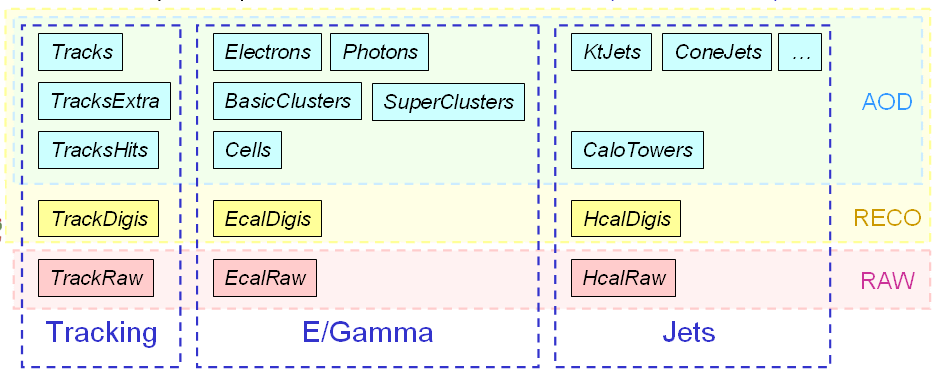
\includegraphics[width=\columnwidth]{gfx/ch2/whats_in_aod_reco.png}
    \caption[Data Tiers]{RAW data is the Detector data after online formatting, the L1 trigger result, the result of the HLT selections (HLT trigger bits), potentially some of the higher level quantities calculated during HLT processing. RECO data contains objects from all stages of reconstruction. AOD are derived from the RECO information to provide data for physics analyses in a convenient, compact format. Most physics analyses can run on AOD data. Courtesy of the CMS public wiki.}
    \label{fig:datatier}
\end{figure}

The AOD format, containing all the relevant physical objects, formed the backbone of the CMS analyses for the entirety of Run 1. However, such an amount of information mean that the typical AOD will store about 400 kB \emph{per event}. This is often redundant for the needs of analysis. Additionally, the increase in luminosity during subsequent runs means that the size of the format will keep increasing: at the end of 2013, the total size of AOD stored by CMS for Run 1 was about 20 petabytes. The CMS collaboration has thus commissioned various new data formats aimed at reducing the size of the analysis data files.
Initially the MiniAOD format was introduced in 2014 (see \cite{Petrucciani_2015}), about one tenth the size of AOD (i.e. 40-60 kB per event), and which has seen a wide adoption by the experiment during Run 2. In recent years, however, the \emph{NanoAOD} format has been proposed \cite{Peruzzi_2020}, with the aim of serving the needs of a substantial fraction of CMS physics analyses with a per-event payload of about 1-2 kB.

NanoAOD achieves such a strong data reduction by retaining only high level information on physics objects, such as jets and leptons, dropping their individual constituents, and reducing the precision of stored variables.
The design rationale of NanoAOD is based on previous experience from \emph{user "ntuples"} and considerations on which minimal set of object information can support a large set of analysis efforts. The introduction of the NanoAOD data format has a dramatic impact on the estimates for computing resources needed by the CMS experiment during the High-Luminosity operation phase of the LHC. Assuming a design target of 50$\%$ analysis coverage with NanoAOD is met by then, the projected needs for disk storage in 2027 are decreased by a factor of about 2, corresponding to a reduction of more than 2 EB (Exabytes). The needed CPU processing power is also decreased by about 15$\%$, as user ntuple production is partially replaced by the central NanoAOD workflow.

Despite this, the potential advantages of the NanoAOD for simulated data are still partially hampered by the current production procedure: NanoAOD can be produced from MiniAOD files at a rate of about 10 events per second on a
single CPU core. This, in turn, means that we are bound to have an underling AOD file, which implies that we still need to perform all the computationally expensive steps of Section \ref{sec:modelling} if we are to simulate our data.
However, the consistently reduced size of the NanoAOD opens up new possibilities for its production thorugh non-conventional, non-\texttt{Geant4} based approaches. 

Specifically, in the present work we are interested in investigating \emph{state-of-the-art deep learning} techniques as a way of bypassing the Simulation, Digitization \emph{and} Reconstruction steps and directly produce new, original events in the NanoAOD format in a fraction of the time and using only a subset of the resources.

\begin{figure}
    \centering
    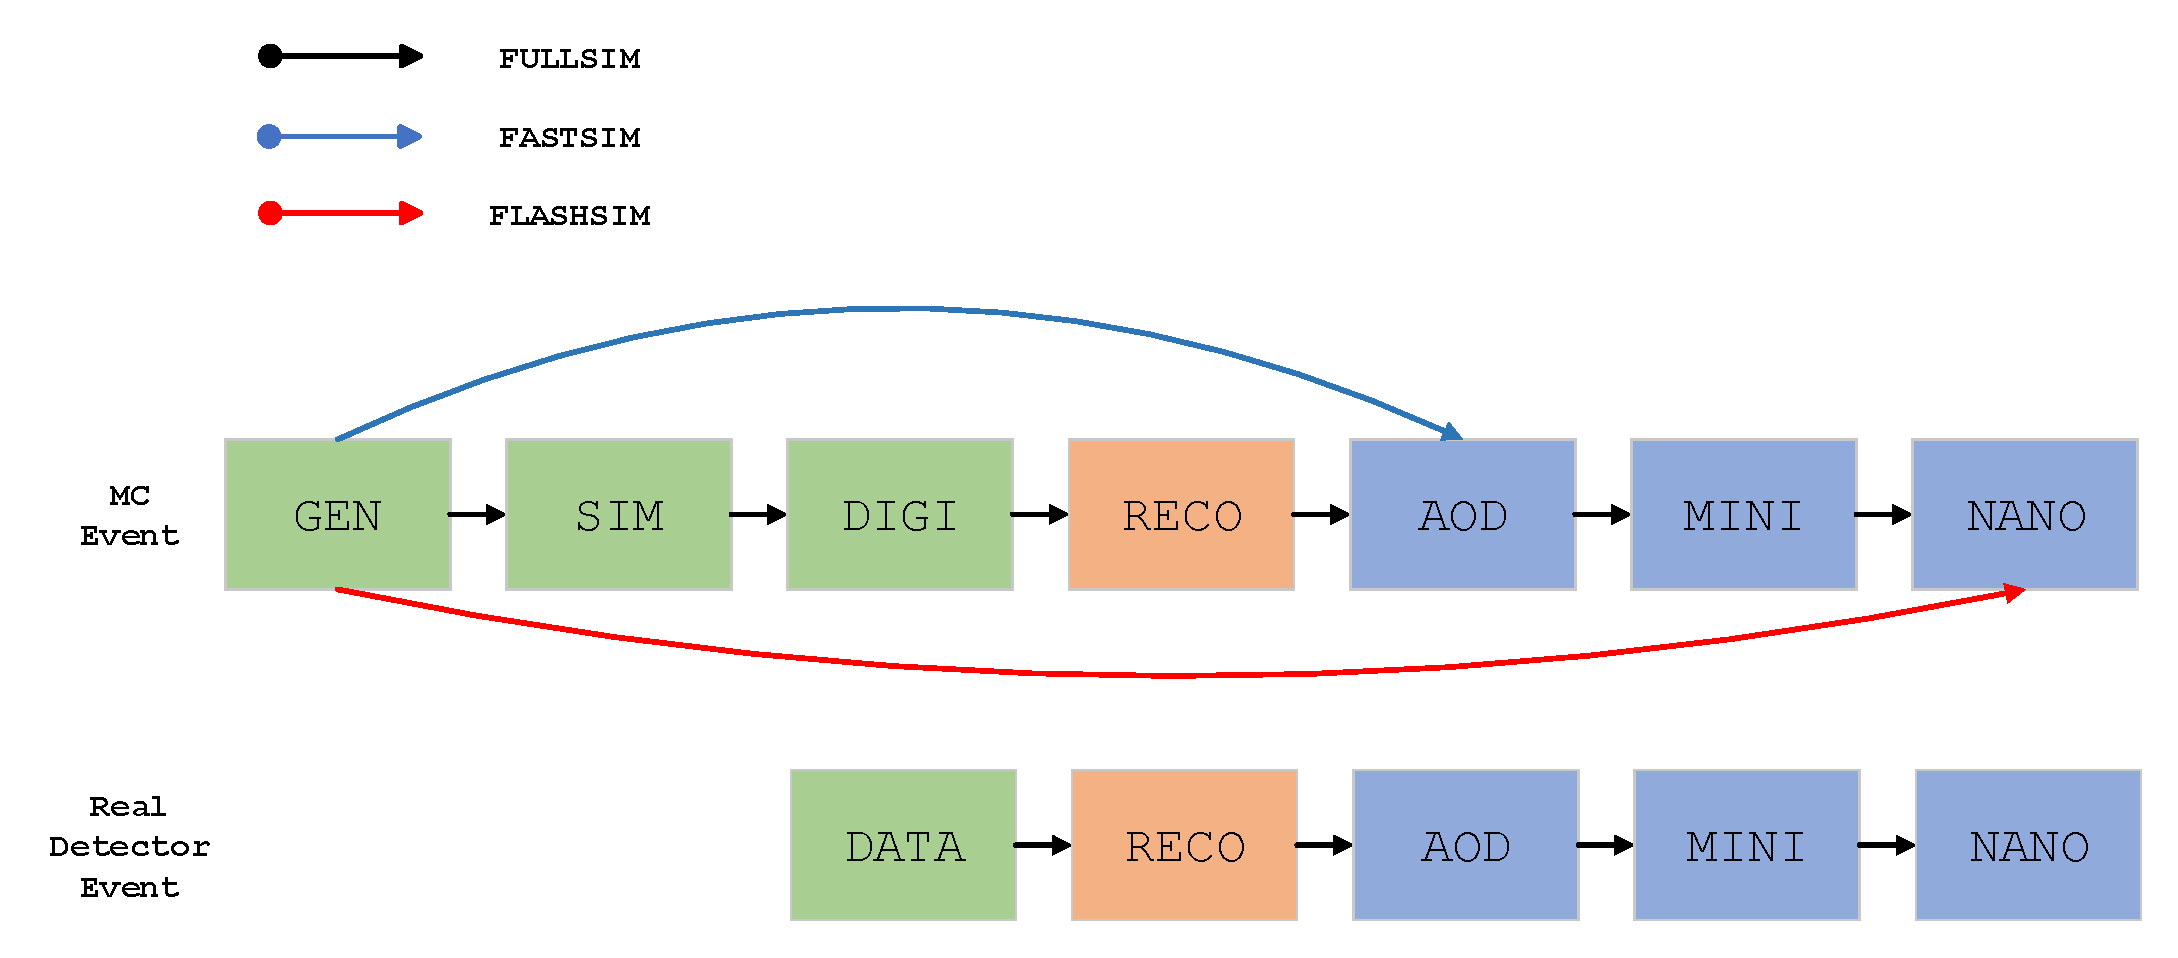
\includegraphics[width=\columnwidth]{gfx/ch2/sim_comp.pdf}
    \caption[Simulation comparison]{The proposed FlashSim would be able of performing realistic NanoAOD production and effectively bypassing all the intermediate steps. The FullSim chain is showed above, along with the CMS FastSim and our FlashSim approaches. We show below the real data processing chain: the RECO and file formats steps are in common between the two.}
    \label{fig:sim_comp}
\end{figure}

The idea behind this approach is simulating only a smaller set of variables. In particular, we would like to retain only high level information, useful to perform physical analyses. This means that the overall complexity of the simulation target has been greatly reduced as we are not interested in precise track or hits reconstruction, for example.

As a final recap of this chapter discussion, we show in Figure \ref{fig:sim_comp} a comparison between the FullSim chain, the FastSim approach and our proposed FlashSim. The real data processing pipeline is also showed underneath.
%*****************************************
%*****************************************
%*****************************************
%*****************************************
%*****************************************

\cleardoublepage
\ctparttext{We move on to describe the building blocks of our work, i.e. \emph{Deep Learning} and specifically \emph{Generative Models}. We conclude with a discussion about the powerful approach know as \emph{Normalizing Flows}. The present part serves both as an high level introduction as well as a way of putting into context the result of the thesis.}
\part{Tools}\label{pt:tools}
%\addtocontents{toc}{\protect\clearpage} % <--- just debug stuff, ignore
%************************************************
\chapter{Normalizing Flows}\label{ch:mathtest} % $\mathbb{ZNR}$
%************************************************
Ei choro aeterno antiopam mea, labitur bonorum pri no. His no decore
nemore graecis. In eos meis nominavi, liber soluta vim cu. Sea commune
suavitate interpretaris eu, vix eu libris efficiantur.

\section{Some Formulas}
Due to the statistical nature of ionisation energy loss, large
fluctuations can occur in the amount of energy deposited by a particle
traversing an absorber element\footnote{Examples taken from Walter
Schmidt's great gallery: \\
\url{http://home.vrweb.de/~was/mathfonts.html}}.  Continuous processes
such as multiple
scattering and energy loss play a relevant role in the longitudinal
and lateral development of electromagnetic and hadronic
showers, and in the case of sampling calorimeters the
measured resolution can be significantly affected by such fluctuations
in their active layers.  The description of ionisation fluctuations is
characterised by the significance parameter $\kappa$, which is
proportional to the ratio of mean energy loss to the maximum allowed
energy transfer in a single collision with an atomic electron:
\graffito{You might get unexpected results using math in chapter or
section heads. Consider the \texttt{pdfspacing} option.}
\begin{equation}
\kappa =\frac{\xi}{E_{\textrm{max}}} %\mathbb{ZNR}
\end{equation}
$E_{\textrm{max}}$ is the maximum transferable energy in a single
collision with an atomic electron.
\[
E_{\textrm{max}} =\frac{2 m_{\textrm{e}} \beta^2\gamma^2 }{1 +
2\gamma m_{\textrm{e}}/m_{\textrm{x}} + \left ( m_{\textrm{e}}
/m_{\textrm{x}}\right)^2}\ ,
\]
where $\gamma = E/m_{\textrm{x}}$, $E$ is energy and
$m_{\textrm{x}}$ the mass of the incident particle,
$\beta^2 = 1 - 1/\gamma^2$ and $m_{\textrm{e}}$ is the electron mass.
$\xi$ comes from the Rutherford scattering cross section
and is defined as:
\begin{eqnarray*} \xi  = \frac{2\pi z^2 e^4 N_{\textrm{Av}} Z \rho
\delta x}{m_{\textrm{e}} \beta^2 c^2 A} =  153.4 \frac{z^2}{\beta^2}
\frac{Z}{A}
  \rho \delta x \quad\textrm{keV},
\end{eqnarray*}
where

\begin{tabular}{ll}
$z$          & charge of the incident particle \\
$N_{\textrm{Av}}$     & Avogadro's number \\
$Z$          & atomic number of the material \\
$A$          & atomic weight of the material \\
$\rho$       & density \\
$ \delta x$  & thickness of the material \\
\end{tabular}

$\kappa$ measures the contribution of the collisions with energy
transfer close to $E_{\textrm{max}}$.  For a given absorber, $\kappa$
tends
towards large values if $\delta x$ is large and/or if $\beta$ is
small.  Likewise, $\kappa$ tends towards zero if $\delta x $ is small
and/or if $\beta$ approaches $1$.

The value of $\kappa$ distinguishes two regimes which occur in the
description of ionisation fluctuations:

\begin{enumerate}
\item A large number of collisions involving the loss of all or most
    of the incident particle energy during the traversal of an absorber.

    As the total energy transfer is composed of a multitude of small
    energy losses, we can apply the central limit theorem and describe
    the fluctuations by a Gaussian distribution.  This case is
    applicable to non-relativistic particles and is described by the
    inequality $\kappa > 10 $ (\ie, when the mean energy loss in the
    absorber is greater than the maximum energy transfer in a single
    collision).

\item Particles traversing thin counters and incident electrons under
    any conditions.

    The relevant inequalities and distributions are $ 0.01 < \kappa < 10
    $,
    Vavilov distribution, and $\kappa < 0.01 $, Landau distribution.
\end{enumerate}


\section{Various Mathematical Examples}
If $n > 2$, the identity
\[
    t[u_1,\dots,u_n] = t\bigl[t[u_1,\dots,u_{n_1}], t[u_2,\dots,u_n]
    \bigr]
\]
defines $t[u_1,\dots,u_n]$ recursively, and it can be shown that the
alternative definition
\[
    t[u_1,\dots,u_n] = t\bigl[t[u_1,u_2],\dots,t[u_{n-1},u_n]\bigr]
\]
gives the same result.

%*****************************************
%*****************************************
%*****************************************
%*****************************************
%*****************************************

%************************************************
\chapter{Normalizing Flows}\label{ch:mathtest} % $\mathbb{ZNR}$
%************************************************

In standard probabilistic modeling practice, we represent our beliefs over unknown continuous quantities with simple parametric distributions like the normal, exponential, and Laplacian distributions. However, using such simple forms, which are commonly symmetric and unimodal (or have a fixed number of modes when we take a mixture of them), restricts the performance and flexibility of our methods. For instance, standard variational inference in the Variational Autoencoder uses independent univariate normal distributions to represent the variational family. The true posterior is neither independent nor normally distributed, which results in suboptimal inference and simplifies the model that is learnt. In other scenarios, we are likewise restricted by not being able to model multimodal distributions and heavy or light tails, widespread in HEP.

\emph{Normalizing Flows} are a type of \emph{latent generative model}, capable of producing new, original samples from a latent space, usually a Gaussian one. The main advantage of this approach, when compared to the previous ones, is that it has been specifically engineered to define explicit \emph{densities}--making it particularly well suited to our use case.

The present chapter serves as a general explanation of the basic concepts and ideas for defining and implementing Normalizing Flows (NF for short). We also briefly discuss in a more general way the possible use cases of this architecture. For the interested reader, an excellent review is the one by Papamakarios et al \cite{papanf}.

\section{Definitions}

Normalizing flows are a family of methods for constructing flexible learnable probability distributions, often with neural networks, which allow us to surpass the limitations of simple parametric forms to represent complex high-dimensional distributions.

\subsection{Basics}

The basic idea is to define a complex distribution $p_x(\mathbf{x})$ by passing \emph{random variables} $\mathbf{z} \in \mathbb{R}^D$ drawn from a simple \emph{base distribution} $p_z(\mathbf{z})$ through a non-linear, \emph{invertible} and \emph{differentiable} transformation \emph{f}: $\mathbb{R}^D \rightarrow \mathbb{R}^D$, $\mathbf{x} = f(\mathbf{z})$. \emph{f} can also be called a \emph{bijection}. The base distribution is usually chosen to be simple, for example a standard i.i.d. normal distribution, $\mathbf{z}\sim\mathcal{N}(\mathbf{0},I_{D\times D})$, which makes it very simple to sample and evaluate. 

We may now use the change-of-variable formula to express $p_x(\mathbf{x})$ as:

\[
p_x(\mathbf{x}) = p_z(\mathbf{z})\det\left|\frac{d\mathbf{z}}{d\mathbf{x}}\right|
\]

and remembering that \emph{f} is invertible, taking the logarithm of both sides we get:

\begin{equation}\label{eqn:logpdf}
	\begin{aligned}
		\log(p_x(x)) &= \log(p_z(f^{-1}(\mathbf{x})))+\log\left(\det\left|\frac{d\mathbf{z}}{d\mathbf{x}}\right|\right)\\
		&= \log(p_z(f^{-1}(\mathbf{x})))-\log\left(\det\left|\frac{d\mathbf{x}}{d\mathbf{z}}\right|\right)
	\end{aligned}
\end{equation}

where $d\mathbf{z}/d\mathbf{x}$ denotes the Jacobian matrix of $f^{-1}(\mathbf{x})$, $\mathbb{J}_{f^{-1}}(\mathbf{x})$.
Intuitively, this equation says that the density of $x$ is equal to the density at the corresponding point in $z$ plus a term that corrects for the warp in volume around an infinitesimally small volume around $x$ caused by the transformation.
	We can compose such bijective transformations to produce even more complex distributions. It is clear that, if we have $K$ transforms $f_{(1)}, f_{(2)},\ldots,f_{(K)}$, then the log-density of the transformed variable $\mathbf{x}=(f_{(1)}\circ f_{(2)}\circ\cdots\circ f_{(K)})(\mathbf{z})$ is:
	
	\begin{equation*}
		\begin{aligned}
			\log(p_x(\mathbf{x})) &= \log\left(p_z\left(\left(f_{(K)}^{-1}\circ\cdots\circ f_{(1)}^{-1}\right)\left(\mathbf{x}\right)\right)\right)+\\
			&+\sum^{K}_{k=1}\log\left(\left|\frac{df^{-1}_{(k)}(\mathbf{x}_{(k)})}{d\mathbf{x}'}\right|\right)
		\end{aligned}
	\end{equation*}
	
This relationship between the base distribution and the transformed one through this chain of invertible transforms is at the core of the NF approach and is illustrated in Figure \ref{fig:nf}.

\begin{figure}
    \centering
    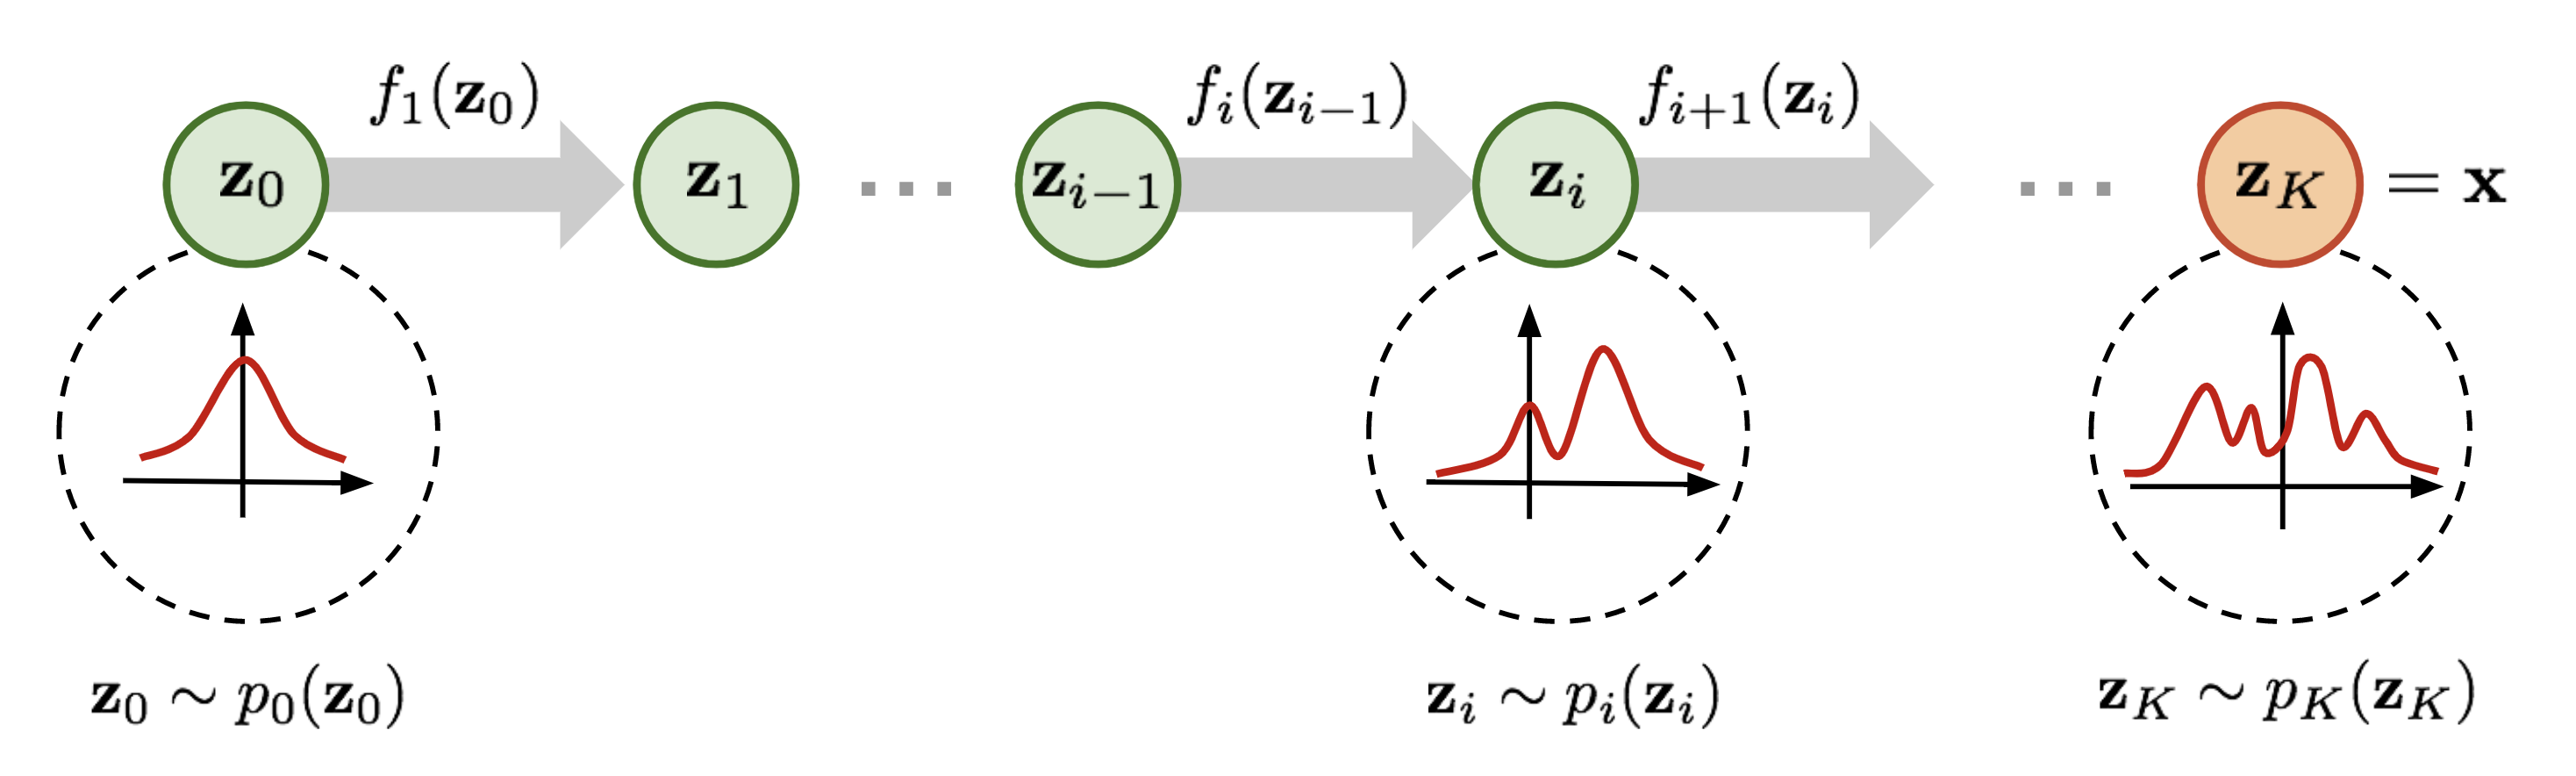
\includegraphics[width=\columnwidth]{gfx/ch4/normalizing-flow.png}
    \caption[Normalizing Flows]{The main idea behind Normalizing Flows: how can we find a chain of invertible transformations to send $p_z(\mathbf{z})$ to $p_x(\mathbf{x})$? Taken from \cite{nffig}.}
    \label{fig:nf}
\end{figure}
	
Based on this, the idea is to define some kind of measure, which can then be used as the objective function to minimize, to learn the optimal transformation \emph{f}.

\subsection{Loss functions}

As the idea is to leverage deep learning, we let our transformation \emph{f} depend on a set of parameters $\phi$, $f = f(\mathbf{x};\, \phi)$.
For the sake of completeness, we distinguish two main cases.

\paragraph{Forward KL Divergence}
Suppose that we have samples from the target distribution (or we are able to generate them), but we cannot evaluate the underlying pdf $p_x^*(\mathbf{x})$. This is precisely our case in HEP, with billions of available Monte Carlo data and no analytical pdf. Then, we may define as our loss function the \emph{forward Kullback-Leibler divergence} between the target distribution $p_x^*(\mathbf{x})$ and the flow-defined one $p_x(\mathbf{x}; \, \phi)$:

\begin{equation}\label{eqn:kldiv}
    \begin{aligned}
    \mathcal{L}(\phi) &= \mathcal{D}_{KL}[p_x^*(\mathbf{x})||p_x(\mathbf{x}; \, \phi)]\\
    &= -\mathbb{E}_{p_x^*(\mathbf{x})}[\log(p_x(\mathbf{x}; \, \phi))] +\; \text{const.}\\
    &= -\mathbb{E}_{p_x^*(\mathbf{x})}[\log(p_z(f^{-1}(\mathbf{x}; \, \phi)))+\log\left(\det\mathbb{J}_{f^{-1}}(\mathbf{x}; \, \phi)\right)] +\; \text{const.}
    \end{aligned}
\end{equation}

where we have used Eq. \ref{eqn:logpdf}. Supposing we had a set of training samples $\{\mathbf{x}\}^N_n$ from the target pdf, we may estimate the expectation value over $p_x^*(\mathbf{x})$ by Monte Carlo as:

\[
\mathcal{L}(\phi) \approx -\frac{1}{N} \sum_n [\log(p_z(f^{-1}(\mathbf{x}; \, \phi)))+\log\left(\det\mathbb{J}_{f^{-1}}(\mathbf{x}_n; \, \phi)\right)] +\; \text{const.}
\]

For computing this loss we need to calculate $f^{-1}$, its Jacobian determinant and the density $p_z(f^{-1}(\mathbf{x}; \, \phi))$. 

\paragraph{Reverse KL Divergence} If instead we have the ability to easily evaluate $p_x^*(\mathbf{x})$ but not to sample from it, the \emph{reverse Kullback-Leibler divergence} is more well suited:

\[
\begin{aligned}
    \mathcal{L}(\phi) &= \mathbb{E}_{p_x(\mathbf{x}, \, \phi)}[\log(p_x(\mathbf{x}; \, \phi)) - \log(p_x^*(\mathbf{x}))]\\
    &= \mathbb{E}_{p_x(\mathbf{x}, \, \phi)}[\log(p_z(\mathbf{z}))-\log\left(\det\mathbb{J}_{f}(\mathbf{x}; \, \phi)\right)-\log(p_x(\mathbf{x}; \, \phi))]
\end{aligned}
\]

\section{Constructing flows}
For an actual implementation, the main challenge is in designing parametrizable multivariate bijections that have closed form expressions for both $f$ and $f^{-1}$, a tractable Jacobian whose calculation scales with $O(D)$ rather than $O(D^3)$, and can express a flexible class of functions.

\subsection{Coupling Layers}\label{sec:couplay}

One simple way to reduce the computational complexity of the Jacobian is to introduce \emph{coupling layers}. The basic idea is illustrated in Figure \ref{fig:coupla}.

\begin{figure}
    \centering
    \scalebox{0.65}{
    \begin{tikzpicture}[
        thick, node distance=15mm,
        set/.style={draw, diamond, text width=8mm, align=center},
        op/.style={draw, circle, text width=5mm, align=center, fill=orange!40},
      ]
    
      \node[set, fill=blue!20] (z1) {$\vec z_{1:d}$};
      \node[op, right=of z1] (eq) {\raisebox{-1ex}=};
      \node[set, right=of eq, fill=blue!20] (x1) {$\vec x_{1:d}$};
      \draw[->] (z1) edge (eq) (eq) edge (x1);
    
      \node[set, below=1 of z1, fill=green!30] (z2) {$\mathclap{\vec z_{d+1:D}}$};
      \node[op, right=of z2] (g) {$f$};
      \node[below=1em of g] (forward) {forward pass};
      \node[set, right=of g, fill=yellow!40] (x2) {$\mathclap{\vec x_{d+1:D}}$};
      \draw[->] (z2) edge (g) (g) edge (x2);
    
      \node[op] (m) at ($(z1)!0.5!(g)$) {$\phi$};
      \draw[->] (z1) edge (m) (m) edge (g);
    
      \begin{scope}[xshift=9cm]
    
        \node[set, fill=blue!20] (z1) {$\vec z_{1:d}$};
        \node[op, right=of z1] (eq) {\raisebox{-1ex}=};
        \node[set, right=of eq, fill=blue!20] (x1) {$\vec x_{1:d}$};
        \draw[<-] (z1) edge (eq) (eq) edge (x1);
    
        \node[set, below=1 of z1, fill=green!30] (z2) {$\mathclap{\vec z_{d+1:D}}$};
        \node[op, right=of z2] (g) {$\mathclap{f^{-1}}$};
        \node[below=1em of g] (inverse) {inverse pass};
        \node[set, right=of g, fill=yellow!40] (x2) {$\mathclap{\vec x_{d+1:D}}$};
        \draw[<-] (z2) edge (g) (g) edge (x2);
    
        \node[op] (m) at ($(x1)!0.5!(g)$) {$\phi$};
        \draw[->] (x1) edge (m) (m) edge (g);
    
      \end{scope}
    
    \end{tikzpicture}}
    \caption[Coupling layer]{The two possible passes through a coupling layer.}
    \label{fig:coupla}
\end{figure}

We partition the input $\mathbf{z} \in \mathbb{R}^D$ into two subsets $(\vec z_{1:d}, \, \vec z_{d+1:D}) \in \mathbb{R}^d \times \mathbb{R}^{D-d}$, where \emph{d} is an integer between 1 and \emph{D}, and is usually taken as $\lceil D/2 \rceil$. Then, at each step, the transformation $f_i$ is defined as:

\[
f_i(\mathbf{z}; \, \phi) = f_i(\vec z_{d+1:D}; \, \phi(\vec z_{1:d}))
\]

that is, the single transformation acts only on a \emph{subset} of the input, keeping the other part unchaged and using it as \emph{conditioning} for the actual parameters. 

At the end, the two subset are joined together to form the input for the next layer; by applying arbitrary permutations between the indexes we can ensure that eventually all values of the input get transformed. What is more, this also means that because we condition on the different indexes of the same input the transformation can correctly learn to model \emph{correlations} between 1d distribution for the same instance.

But the greatest advantage is that now the single transformation depends only on one subset of inputs, and thus its jacoban is \emph{block triangular}:

\[
\mathbb{J}_{f}(\mathbf{x}; \, \phi) = 
\begin{pmatrix}
\frac{\partial \vec x_{1:d}}{\partial \vec z_{1:d}} & \frac{\partial \vec x_{1:d}}{\partial \vec z_{d+1:D}}\\
\frac{\partial \vec x_{d+1:D}}{\partial \vec z_{1:d}} & \frac{\partial \vec x_{d+1:D}}{\partial \vec z_{d+1:D}}
\end{pmatrix}
=
\begin{pmatrix}
\mathbb{I} & 0\\
A & \mathbb{J}^*
\end{pmatrix}
\]

The full Jacobian determinant can simply be calculated from the product of the diagonal elements of $\mathbb{J}^*$, which are simply the partial derivatives over ($d+1, \dots D$). A similar reasoning holds for the Jacobian of the inverse.
This significantly speeds up the calculations.

\subsection{Splines}

There are many possible bijections which one can use in building a NF. Recent advancements have demonstrated the suitability of \emph{rational-quadratic spline transforms} (see \cite{durkan}). 

A monotonic spline is a piecewise function consisting of K segments, where each segment is a simple function that is easy to invert. Specifically, given a set of K+1 input locations $l_{0}, \dots, l_K$ , the transformation
is taken to be a simple monotonic function (e.g. a low-degree polynomial) in each interval
[$l_{k}, l_{k+1}$], under the constraint that the K segments meet at the endpoints.
Outside the interval [$l_{0}, l_K$], the transformer can default to a simple function such as the
identity. Typically, the parameters $\phi$ of the transformations are the input locations, 
the corresponding output locations and (depending on the type of spline) the
derivatives (i.e. slopes) at $l_{0}, \dots, l_K$. An example is illustrated in Figure \ref{fig:rqs}.

\begin{figure}
    \centering
    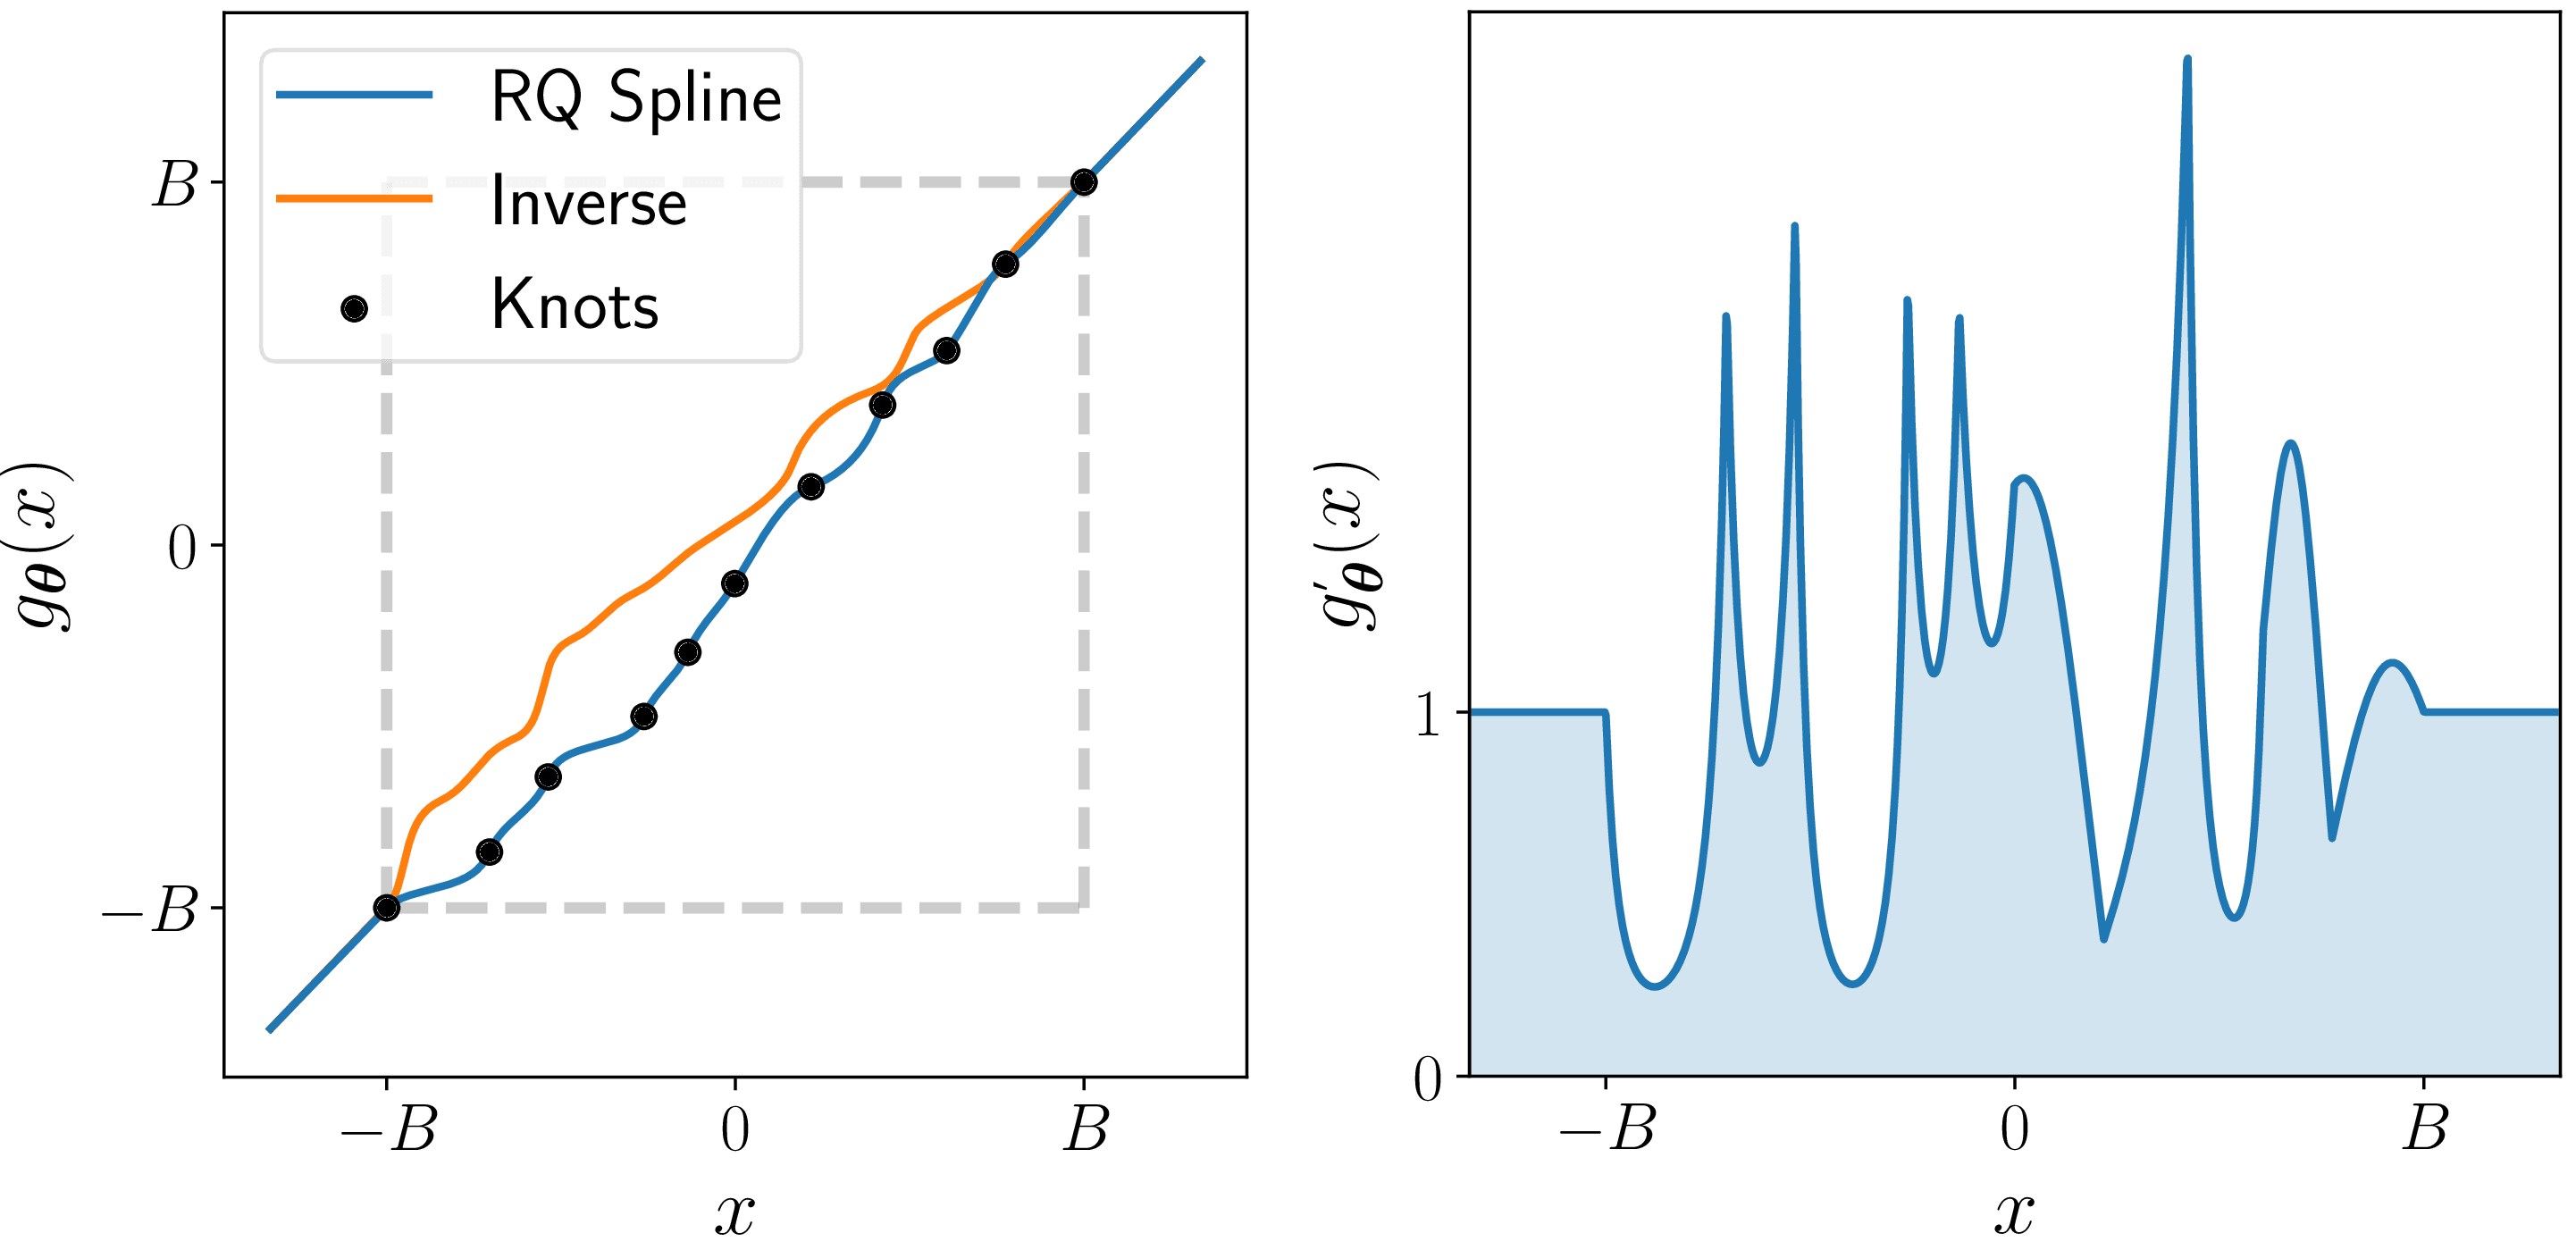
\includegraphics[width=\columnwidth]{gfx/ch4/D9F0PDyWsAAWKHf.png}
    \caption[Rational quadratic spline]{A rational quadratic spline $g_{\theta}(x)$ and its derivative $g_{\theta}^{'}(x)$}
    \label{fig:rqs}
\end{figure}

Spline-based transformers are as fast to invert as to evaluate, while
maintaining exact analytical invertibility. Evaluating or inverting a spline-based transformer
is done by first locating the right segment--which can be done in $\mathcal{O}$(log K) time using binary
search—and then evaluating or inverting that segment, which is assumed to be analytically
tractable. By increasing the number of segments K, a spline-based transformer can be
made arbitrarily flexible.

\subsection{Conditional distributions}

The theory of Normalizing Flows is also easily generalized to conditional distributions. We denote the variable to condition on by $C=\mathbf{c}\in\mathbb{R}^M$. A simple multivariate source of noise, for example a standard i.i.d. normal distribution, $\mathbf{z}\sim\mathcal{N}(\mathbf{0},I_{D\times D})$, is passed through a vector-valued bijection that also conditions on C, $f:\mathbb{R}^D\times\mathbb{R}^M\rightarrow\mathbb{R}^D$, to produce the more complex transformed variable $\mathbf{x}=f(\mathbf{z};\, \phi(C))$. 

In practice, this is usually accomplished by making the parameters for a known normalizing flow bijection $f$ the output of a neural network that inputs $\mathbf{c}$ as well as one of the subsets of the coupling layer. It is thus straightforward to condition event generation on some ground truth, e.g. the Monte Carlo Gen values matched to our targets.


\section{Applications}\label{sec:nfapp}

The use cases of Normalzing Flows are numerous. 
Here we simply limit ourselves to those that we deem more interesting from the point of view a physicist.

\paragraph{Density estimation and generation}

Due to their ability to be expressive while still allowing for exact likelihood calculations, Normalizing Flows are often used for probabilistic modeling of data. For this application, we assume access to a finite number of draws $\mathbf{x})$ from some unknown generative process $p^*_x(\mathbf{x})$. We then train the Flow according to Eq. \ref{eqn:kldiv}: we can now use the model to estimate densities, expectations, marginals, or other quantities of interest on never-before-seen data; as well as sampling from the model novel instances that could have plausibly been sampled from $p^*_x(\mathbf{x})$. The latter use case, generation, has been a popular application of flows in machine learning, for various categories of data. It is also the one upon which the present work is based.

\paragraph{Inference}
We can also turn to \emph{inference}: estimating unknown quantities within a model. The most common setting is the computation of high-dimensional, analytically intractable integrals of the form: 

\[
\int \text{d}\eta \pi(\eta)
\]

as, for example, the posterior’s normalizing constant or when computing expectations under the posterior in Bayesian inference. Common approaches to this problem include \emph{importance sampling}, where integrals are converted to an expectation under an auxiliary distribution $q(\eta)$:

\[
\int \text{d}\eta \pi(\eta) = \int \text{d}\eta q(\eta) \frac{\pi(\eta)}{q(\eta)} \approx \frac{1}{S}\sum_s \frac{\pi(\eta_s)}{q(\eta_s)}
\]

where $q(\eta)$ is a user-specified density function and $\eta_s$ is a sample from $q(\eta)$. Clearly, this requires both sampling and density evaluation. Since both operations are tractable for many
flows, they make for an attractive model from which to construct the proposal.
Additionally, Flows may also be employed as part of \emph{rejection sampling}, \emph{Markov chain Monte Carlo} and \emph{Variational Inference}, to fit distributions over latent variables or model parameters.

\paragraph{Anomaly detection}

Finally, one last application, which proved successful in the recent LHC Olympics \cite{Kasieczka_2021}, is that of \emph{anomaly detection}, aimed at revealing anomalous feature of data signalling potentially new and insightful physical processes.

The best performance on the first black box in the LHCO challenge, as measured by finding and correctly characterising the anomalous signals, was by a team of cosmologists at Berkeley (George Stein, Uros Seljak and Biwei Dai) who compared the phase-space density between a sliding signal region and sidebands using Flows to model the densities directly from data.

%*****************************************
%*****************************************
%*****************************************
%*****************************************
%*****************************************

\cleardoublepage
\ctparttext{You can put some informational part preamble text here.
Illo principalmente su nos. Non message \emph{occidental} angloromanic
da. Debitas effortio simplificate sia se, auxiliar summarios da que,
se avantiate publicationes via. Pan in terra summarios, capital
interlingua se que. Al via multo esser specimen, campo responder que
da. Le usate medical addresses pro, europa origine sanctificate nos se.}
\part{Thesis contribution}\label{pt:thcont}
%************************************************
\chapter{Flash simulation of samples with Normalizing Flows}\label{ch:fs} % $\mathbb{ZNR}$
%************************************************

Having discussed the importance and the challenges of event simulation at LHC, and having described the Deep Learning Normalizing Flows approach, we dedicate this chapter to the practical implementation of an end-to-end sample generator.
The idea is to use NF models to \emph{learn} the mapping from our inputs (noise and generator-level information) to our outputs, consisting in the final-reduction NanoAOD data format for the fully reconstructed data. Having learned the appropriate mapping, the generation of new samples is then trivial, as it consists of sampling a multidimensional Gaussian and adding the relevant generator information. This effectively means being able to skip both the FullSim simulation step, based on \texttt{Geant4}, as well as the reconstruction and readout steps. The following chapter thus describes the variables chosen as inputs and as outputs of our networks, presenting and discussing the results obtained.

The technicalities regarding the actual code implementation are briefly discussed in the Appendix \ref{ch:appx}, and the code use is hosted and documented in detail online \href{tbd}{at the following repository}\footnote{repository link, tbd}.

\section{Target variables}

As we discussed in Section \ref{sec:targets}, we choose to target the VBF Channel of H$\rightarrow\mu^+\mu^-$. Thanks to the clear signature, we only needed to simulate jets and muons out of all the possible objects in a NanoAOD. The present section serves as a discussion of the chosen variables to be simulated with our approach.

For training our model, however, we turned to the t$\overline{\text{t}}$ process. This is an ideal sample, as it contains many different physical processes. What is more, we actually expect our approach to be \emph{independent} from the actual Gen-process, as we are actually learning to model the \emph{detector response} to an arbitrary input: the t$\overline{\text{t}}$ then offers the advantage of already having billions of simulated events ready to be used for a general-purpose training.

\subsection{The t$\overline{\text{t}}$ process}
With a cross-section of $\approx 900$ pb at 13 TeV , the t$\overline{\text{t}}$ process is also \emph{the dominant SM background to many searches for new
physical phenomena}, and its precise measurement is essential for claiming new discoveries.
Inclusive and differential cross section measurements from
proton-proton (pp) collisions at centre-of-mass energies of 13 TeV have been reported by
the CMS collaboration in \cite{Sirunyan_2017}.


Top quarks decay almost exclusively into a W boson and a b quark. The W may then decay in either a q$\overline{\text{q}}$ or a lepton and its corresponding neutrino, ensuring that the events will be well populated with both jets and muons, our simulation targets. 

%\begin{figure}
    %\centering
    %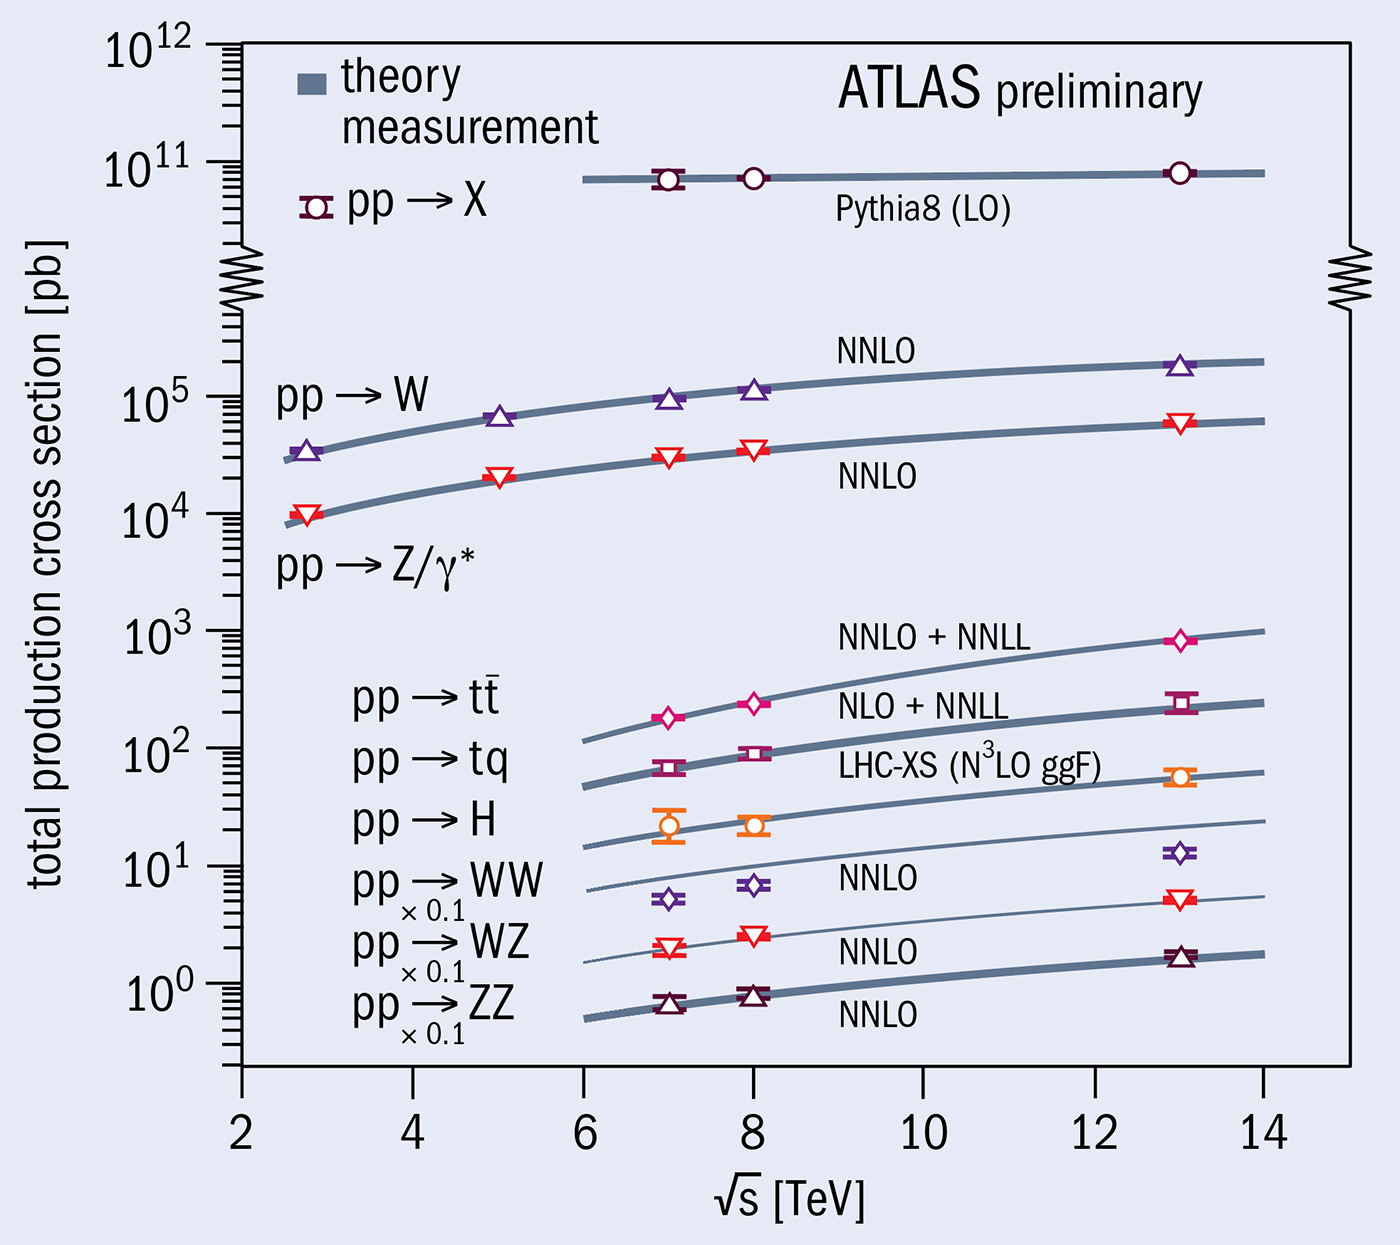
\includegraphics[scale=0.2]{gfx/ch5/CCMarApr_LHC10_fig2.jpg}\quad
    %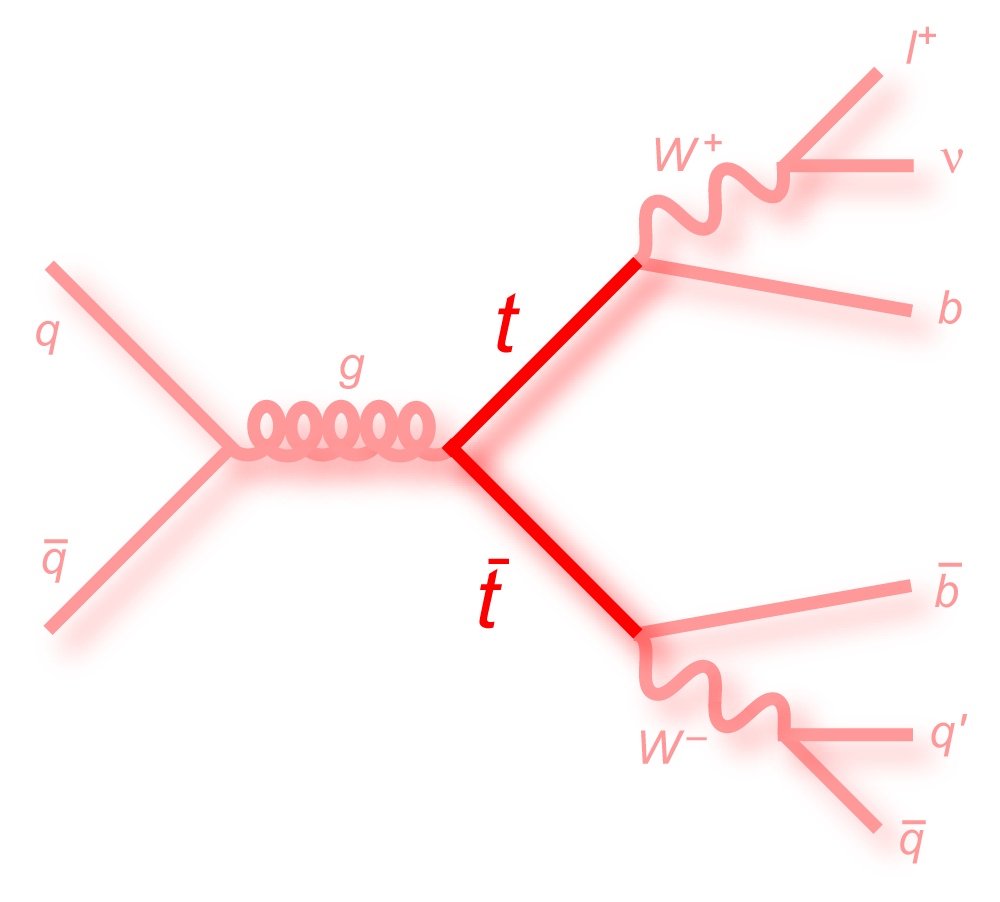
\includegraphics[scale=0.3]{gfx/ch5/feynman_ttbar_ljets_longt.png}
    %\caption[t$\overline{\text{t}}$ diagram]{ The t$\overline{\text{t}}$ process is dominating the cross sections at LHC, making it one of the leading SM background processes. Bottom: the production diagram for proce}
    %\label{fig:ttfig}
%\end{figure}

Having at our disposal a large set of FullSim MC NanoAOD samples for t$\overline{\text{t}}$ events, we used these to \emph{train} our models on the two target objects.

\subsection{Jets}

As discussed in Section \ref{sec:nanoaod}, a NanoAOD, i.e. the CMS standard analysis format, contains both the Jet objects, i.e. final-state reconstructed jets, and the GenJet objects, the jets resulting from the clustering of initial, Gen-level particles before going through the reconstruction step. The latter are either matched to Jet objects, or may end-up unmatched because of limitations in the matching algorithms and the previous simulation steps. For the moment, we disregard the problem of \emph{fake jets}, that is Jet objects which are not matched to a GenJet object but are instead due to noise or Pile-Up.

The idea is being able to directly generate correctly distributed Jet objects starting from noise, for stochasticity,  but also from the values of a corresponding GenJet, as a physical-informed input for the network (a process known as \emph{conditioning}): knowing just the generator-level information of some process, we are going to skip the Simulation, Digitization and Reconstruction steps.


With the use of \texttt{C/C++} code for the \texttt{ROOT} data analysis framework \cite{Brun:491486}, we processed the NanoAOD files and extracted all the Jet objects matched to a GenJet object, across all the events in the file. Because of the large number of variables, we selected a meaningful subset, containing all the necessary information for our test analysis.

First of all, we selected the following 14 GenJet variables for conditioning the generation: 

\begin{outline}
\1 \emph{The physical properties} of the GenJet, that is $\eta$, $\phi$, $m_j$, $p_T$, and the \emph{Parton} and \emph{Hadron Flavour}, giving the \emph{flavour} content of a jet as containg a specific quark or some gluons;

\1 \emph{Variables correlated with the rest of the event}, as the actual properties of a jet are expected to be influenced by other objects such as muons. Computing the $\Delta$R separation between the GenJet and the GenMuons present in the event, we selected the first and second \emph{closest muons}, and we computed the following quantities for each one:
\2 \texttt{Dr}, giving the separation from the GenJet, \texttt{DEta}, the $\eta$ difference from the GenJet, \texttt{DPt}, the $p_T$ difference from the GenJet, \texttt{DPhi}, the $\phi$ difference from the GenJet;

\1 If no GenMuons were present within a cone of $\Delta$R = 0.5 from the GenJet, the corresponding values were set to a user-defined maximum.

\end{outline}

Then, we selected the following 17 target reconstructed variables for the matched reconstructed Jet objects:

\begin{outline}
\1 \emph{The physical properties} of the Jet \emph{with regard to} the ones of the matched GenJet: $\Delta\eta$, the $\eta_{reco} - \eta_{gen}$ difference , $\Delta\phi$, the $\phi$ difference, $R_m$, the ratio of the jet and GenJet masses, $R_{p_T}$, the ratio of $p_T$s. This was done because the Simulation and Reconstruction steps are expected to introduce corrections w.r.t. the GenJet distributions, easier to learn when considering these quantities. As an additional variable, the Jet \texttt{Area}, a measure of its susceptibility to radiation, like pileup or underlying event, was added as well;

\1 Some of the btag discriminant variables \emph{b-tagging and c-tagging algorithms scores}: \texttt{btagCMVA}, \texttt{btagCSVV2}, \texttt{btagDeepB}, \texttt{btagDeepC}, \texttt{btagDeepFlavB} and \\\texttt{btagDeepFlavC}, which indicate with a score ranging from 0 to 1 whether the Jet contains the respective quark or not, a very significant information for performing event selection during an analysis. Some values may be offsetted to -1 to indicate that the corresponding tagging algorithm has faild to assign a score to the event;

\1 The \texttt{bRegCorr}, the $p_T$ correction for b-jet energy regression, as the presence of neurinos due to semi-leptonic decays in the jets coming from b quarks can result in underestimated jet energy measurements;

\1 The \texttt{qgl} score for the Quark vs Gluon likelihood discriminator, which is employed as most of the interesting physics channels studied at the LHC involve hadronic jets initiated by quarks, while dominant backgrounds often arise from QCD events, where jets are generally produced from gluons;

\1 The \texttt{jetID} and \texttt{puID} ID flags indicating relevant characteristics of the jet as well as the event noise and Pile-Up.
\end{outline}
\subsection{Muons}

For muons we performed the same procedure, taking only those muons matching to GenMuon objects (a GenParticle object with pdgId value of $\pm$13). 

We selected 30 GenMuon variables for conditioning:

\begin{outline}
\1 \emph{The physical properties} of the GenMuon, that is $\eta$, $\emph{phi}$, \texttt{Charge} and $p_T$;

\1 \emph{The 14 GenParticle status flags}, a series of \texttt{statusFlags} stored bitwise, with each bit having a different physical interpretation such as \emph{isTauDecayProduct}, \emph{fromHardProcess}, etc. or some information regarding the position of the object in the detector;

\1 \emph{Variables correlated with the rest of the event}, as the actual properties of a muon are expected to be influenced by other objects such as jets. Computing the $\Delta$R separation between the GenMuon and the GenJets present in the event, we selected the first \emph{closest GenJet}, and we computed the following quantities:
\2 $\Delta$R, giving the separation from the GenJet, $\Delta\eta$, the $\eta_{muon} - \eta_{jet}$ difference, $R_{p_T}$, the ratio of $p_T$s, $\Delta\phi$, the $\phi$ difference, and finally the $m_j$ of the closest GenJet;

\1 A series of 6 \emph{ Event level variables regarding Pile-Up}:\\ \texttt{Pileup\_gpudensity}, the Generator-level PU vertices/mm,\\ \texttt{Pileup\_nPU}, the number of pileup interactions that have been added to the event in the current bunch crossing, \texttt{Pileup\_nTrueInt}, the true mean number of the poisson distribution for this event from which the number of interactions each bunch crossing has been sampled, \texttt{Pileup\_pudensity}, PU vertices/mm, \texttt{Pileup\_sumEOOT}, the number of early out of time pileup and \texttt{Pileup\_sumLOOT}, the number of late out of time pileup;
\end{outline}

Then we selected 22 target variables for the Muon objects:

\begin{outline}
\1 \emph{The physical properties} of the muon \emph{with regard to} the ones of the matched GenMuon: \texttt{EtaMinusGen}, the $\eta$ difference , \texttt{PhiMinusGen}, the $\phi$ difference, \texttt{PtRatio}, the ratio of $p_T$s. This was done because the Simulation and Reconstruction steps are expected to introduce corrections w.r.t. the GenMuon distributions, easier to learn when considering these quantities. As an additional variable, the \texttt{ptErr}, the $p_T$ error for the muon track, was selected as well;

\1 Six \emph{impact parameters} with respect to the primary vertex: \texttt{dxy}, \texttt{dxyErr}, \texttt{dz}, \texttt{dzErr}, the 3D impact parameter \texttt{ip3d} and its significance \texttt{sip3d}, all expressed in cm;

\1 Some \emph{Boolean flags}: \texttt{isGlobal}, \texttt{isPFcand}, identifying the muon as a Particle Flow candidate, \texttt{isTracker};

\1 A series of \emph{isolation variables} returned by the Particle Flow algorithm: \texttt{pfRelIso03\_all}, \texttt{pfRelIso03\_chg} and \texttt{pfRelIso04\_all};

\1 The \emph{variables related to the closest jet}: \texttt{jetPtRelv2}, indicating the relative momentum of the lepton with respect to the closest jet after subtracting the lepton and \texttt{jetRelIso}, the relative isolation in matched jet;

\1 A series of \emph{ID scores}: \texttt{mediumID}, \texttt{softMVA} score and its cut-based ID \texttt{softMVAId}, \texttt{softId};
\end{outline}

\subsection{Extraction and preprocessing}

With the use of \texttt{C/C++} code (name of script) for the \texttt{ROOT} data analysis framework \cite{Brun:491486}, we processed the NanoAOD files and extracted all the Jet objects matched to a GenJet object and the Muon objects matched to a GenMuon across all the events in the file. This operation can be performed rather quickly thanks to the \emph{compiled} language being used and the powerful \texttt{ROOT::RDataFrame()} class, offering a modern, high-level interface for the manipulation of data stored in a NanoAOD \texttt{TTree}, as well as \emph{multi-threading} and other low-level optimisations.
The output of the \emph{extraction} step is another \texttt{.root} file containing just the selected objects.

The resulting file is still organized according to the Events structure. Besides, we know that many machine learning algorithms work best when specific distributions are \emph{preprocessed} according to specifc criteria. Normalizing Flows are no exception. Specifically, there are four key features which should be accounted for and modified through preprocessing before training:

\begin{figure}
    \centering
    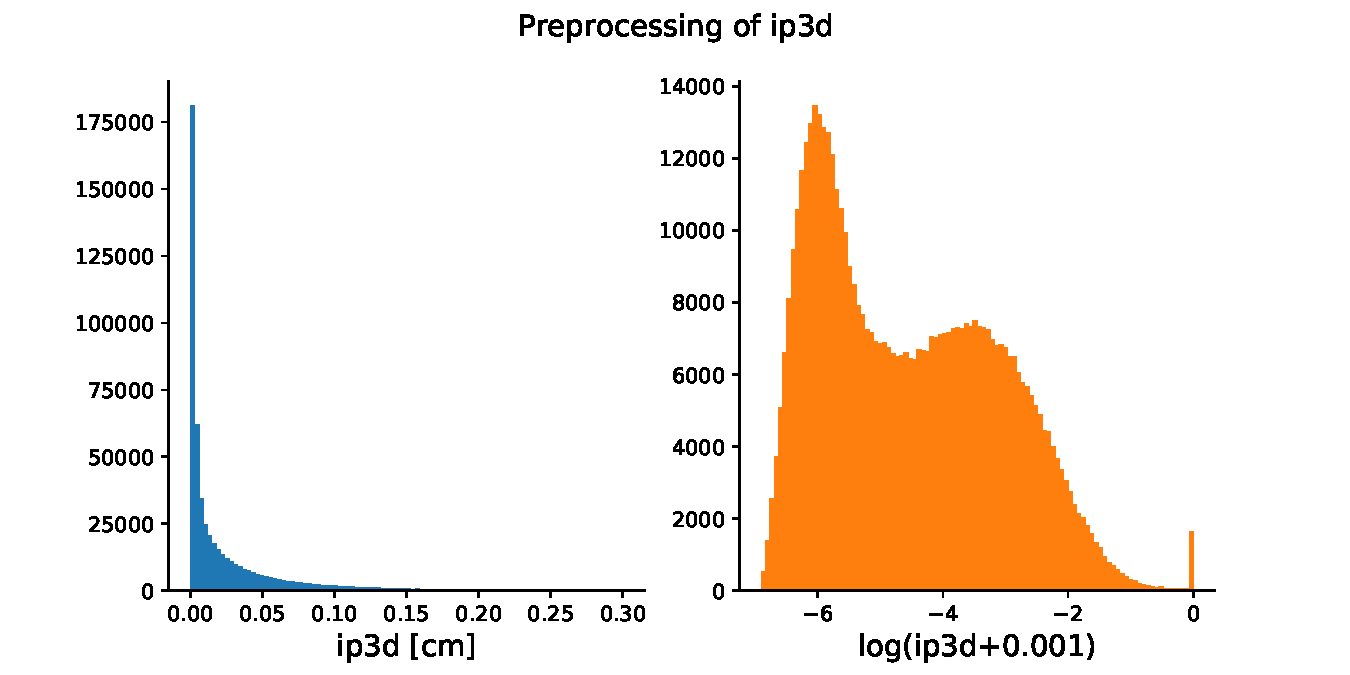
\includegraphics[width=\columnwidth]{gfx/ch5/preproce.pdf}
    \caption[Preprocessing]{Sharply peaked distribution are being converted to more broad ones during the preprocessing step. In this example the \texttt{ip3d} variable gets transformed as log(\texttt{ip3d}+0.001).}
    \label{fig:preproce}
\end{figure}

\begin{outline}
\1 Because NF are learning actual pdfs, \emph{large gaps} between values of the distribution may disturb training and trick the network to \emph{bridge} the extremes of the distribution by creating spurious samples in the gap. When possible, the gaps should be reduced and the values packed closer together;

\1 As NF work with pdfs, they are not well suited to deal with \emph{discrete} distributions. Thus, we should apply a process known as \emph{dequantization}, that is applying some sort of smearing to the discrete values to make them similar to those sampled from a continuous distribution;

\1 For similar resons as before, when possible it would be beneficial to widen and normalize sharply peaked distributions through invertible transforms such as log(x). If well separated, eventual peaks may be dequantized as well;

\1 Finally, we opted for \emph{saturating} long tails of distributions to some limiting values, in order to make it easier for the model to learn the pdf in the more populated region.
\end{outline}

Apart from possibly dequantization, we stress that all of this transformations were implemented to make training easier but are not strictly necessary--the models revealed themselves as powerful enough to deal with complex, sharply peaked, long tailed distributions. However, having already implemented the preprocessing pipeline and because it did not introduce a big overhead in the procedure, we decided to keep it for the present work. An example of one of the possible preprocessing operations is shown in Figure \ref{fig:preproce}.

All of these transforms may be implemented with a clear and natural syntax in the \texttt{Python} programming language, specifically thanks to the \texttt{pandas} package \cite{reback2020pandas}, which implements a convenient dataframe structure. We thus open the \texttt{.root} file directly in a \texttt{Python} script through the \texttt{uproot} package \cite{jim_pivarski_2022_6791281}, discard the Events structure to obtain a simple table with one object per line, perform the preprocessing as discussed above and save the output in \texttt{.hdf5} format for the training.

\section{Models design}
This section describes the implementation  details for the two architectures--the one responsible for the generation of jets and the one targeting muons. We discuss the software choices and then the model specifics and trainings.

\subsection{Software and packages}

We initially planned to use another class of generative models, that is Generative Adversarial Networks. However, after discovering the work of Dr. Stephen Green \cite{stephen_green_2021_4558988} we realized that Normalizing Flows were better suited to our task, as they suffered from less training instabilities and allowed us to directly learn the underlying distributions with an easily interpretable loss function.

The models are implemented following Dr. Green's example: the \texttt{Python} package \texttt{nflows} \cite{conor_durkan_2020_4296287} defines the Classes for Rational Quadratic Spline Normalizing Flows, integrating them for use with the popular ML research package \texttt{Pytorch} \cite{NEURIPS2019_9015}. We obviously had to perform several attempts to optimize the hyperparameters choices for our use case, a long and complicated process which resulted in the architectures presented below.

\subsection{Architectures and trainings}

\begin{figure}
    \centering
    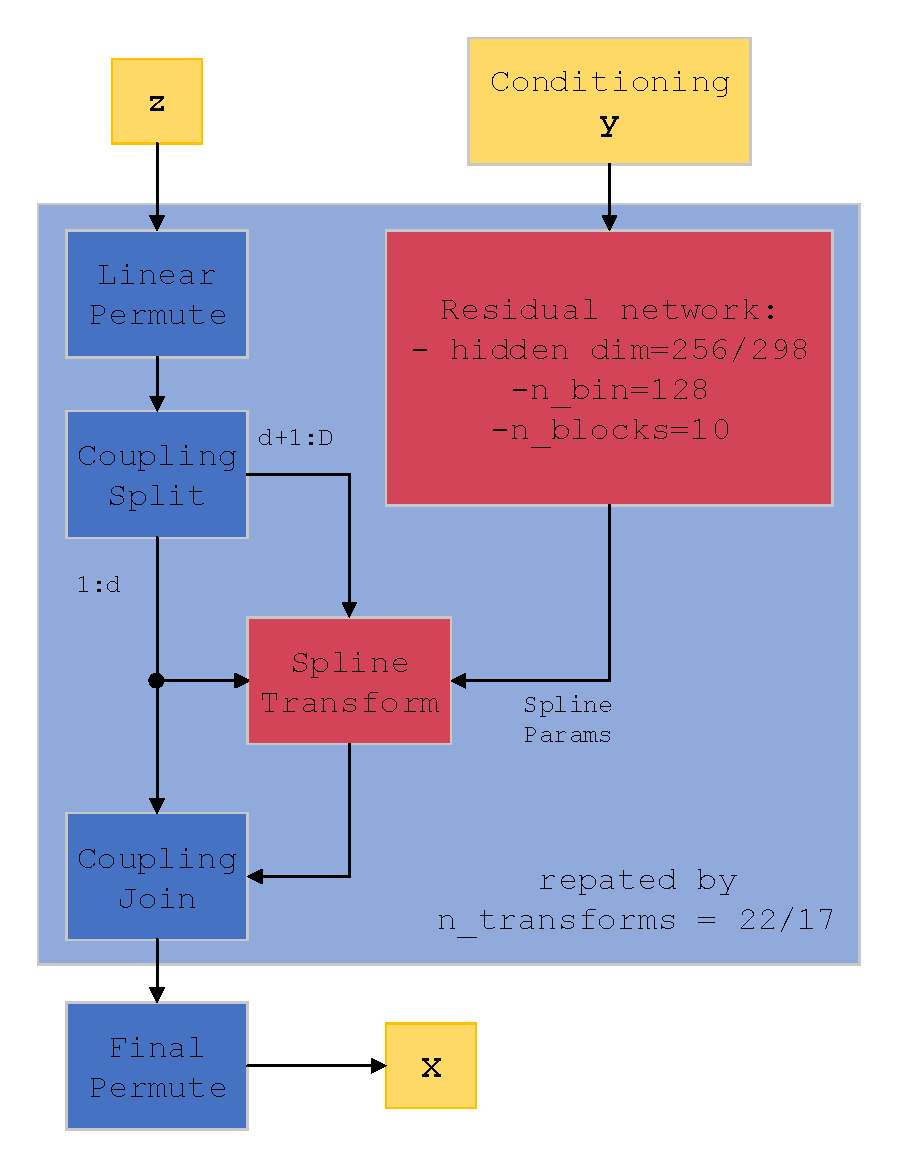
\includegraphics[width=\columnwidth]{gfx/ch5/nfmodel.pdf}
    \caption[Actual NF model]{The NF models are quite large and complex. A number of transforms equal to that of the target variables is performed. The normally distributed inputs \textbf{z} are permuted for each step and then splitted in half, sending half as parameters and half as argument of the \emph{spline transform}. The conditioning variables \textbf{y} are sent as input to a complex 10 layer residual network (different for each transform) which defines the parameters for the spline. Everithing is repeated until the last step where we permute back to the original order and output the targets \textbf{x}. Where two numbers are separetad by a slash, the first refers to the muons model, the second to the jets one.}
    \label{fig:nfmodel}
\end{figure}

Figure \ref{fig:nfmodel} shows the final models employed in this work. 
As discussed in Section \ref{sec:couplay}, in order to reduce the computational complexity of the Jacobian in the NF loss function, we implemented the total transformation as a chain of single, subsequent splines transformations, each acting on just half of the input, while the latter half is kept unchanged and serves as additional parameters for the splines. This has the additional advantage of ensuring good \emph{correlations} between the various variables, as the transformation for one of them will end up depending on every other variable as long as we implement a number of transformation equal to the number of variables and we permute the order linearly before each spline.

For each spline, the normally distributed inputs \textbf{z} are permuted and then splitted in half, sending half as parameters and half as argument of the \emph{spline transform}. The conditioning Gen-level variables \textbf{y} are sent as input to a complex 10 layer fully-connected \emph{residual} network (a different one for each transform) which defines the parameters for the spline. Its most relevant hyperparameters are the \emph{hidden\_dim}, the number of nodes per hidden layer, set to 256 for the muons model and to 298 for the jets one, the \emph{n\_bin}, the number of bins for the spline, set to 128 for both models and the \emph{n\_blocks} set to 10 for both and defining the number of hidden layers.
Each network was defined with \texttt{ReLU} activation function and setting \texttt{batch\_norm=True}. The training procedure actually traverse the network in the opposite way, strarting from the training data and using the inverse transform to obtain normally distributed instances which can easily be evaluated in the NF loss function.

We would like to emphasize the fact that because \emph{each transform} defines a separate network for learning the optimal spline parameters, the final models are quite large, especially for physics-based application standards. The muons model exceeds 54e6 trainable parameters (54,988,164 parameters, corresponding to the various weights of the neurons in each layer and the batch norm parameters), while the jets model totals in at 47,986,595 parameters. These large models were trained on around 5e6 muons or jets objects extracted as explained above, and the \emph{losses} were monitored at each epoch on a separate \emph{validation set} of about 4e5 samples to ensure that the models were not being over-optimized for the training set. Additionally, we saved the model state every 10 epochs and performed additional validation on a separate set of 1e5 data to further avoid overfitting.

As our \emph{optimizer} algorithm we choose the de-facto standard in the field, the \texttt{Adam} algorithm \cite{https://doi.org/10.48550/arxiv.1412.6980}, a complex and powerful algorithm for models optimization still based on the same basic principles of \emph{gradient descent} explained in Section \ref{sec:backprop}, with an initial \emph{learning rate} of 1e-4 for muons and 1e-5 for jets, reduced during training by the \emph{cosine annealing} procedure. The maximum epochs were set to 1000 for the muons model, giving its larger number of target variables, and to 500 for the jets one--this also means that the learning rate reduction due to cosine annealing will be different over training as it depends on the total epochs number.

Trainings were stopped respectively at epoch 580 for muons and at epoch 420 for jets, as we had reached a good convergence, despite both models showing signs for more improvements. Figure \ref{fig:losses} shows the models losses over the training epochs. The validation loss is plotted by averaging over the last 5 epochs, to display the overall trend instead of single, noisy variations. The values on the y-axis are the actual loss values, and they are obviously different as they depend on both the number and the ranges of the target variables.


\begin{figure}
    \myfloatalign
    \subfloat[]
    {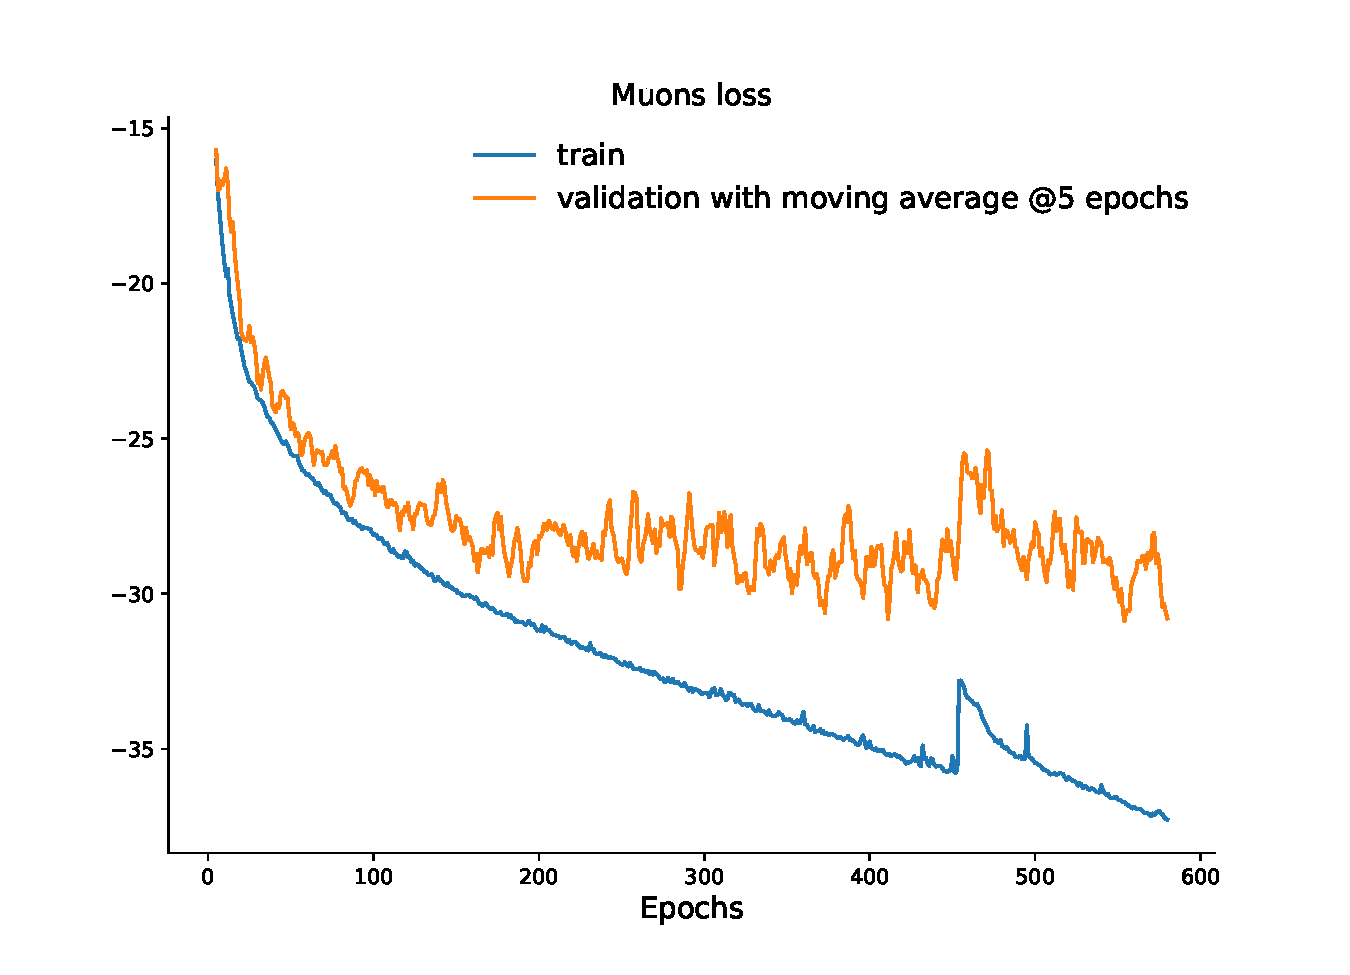
\includegraphics[width=\linewidth]{gfx/ch5/lossesmuons.pdf}} \\
    \subfloat[]
    { 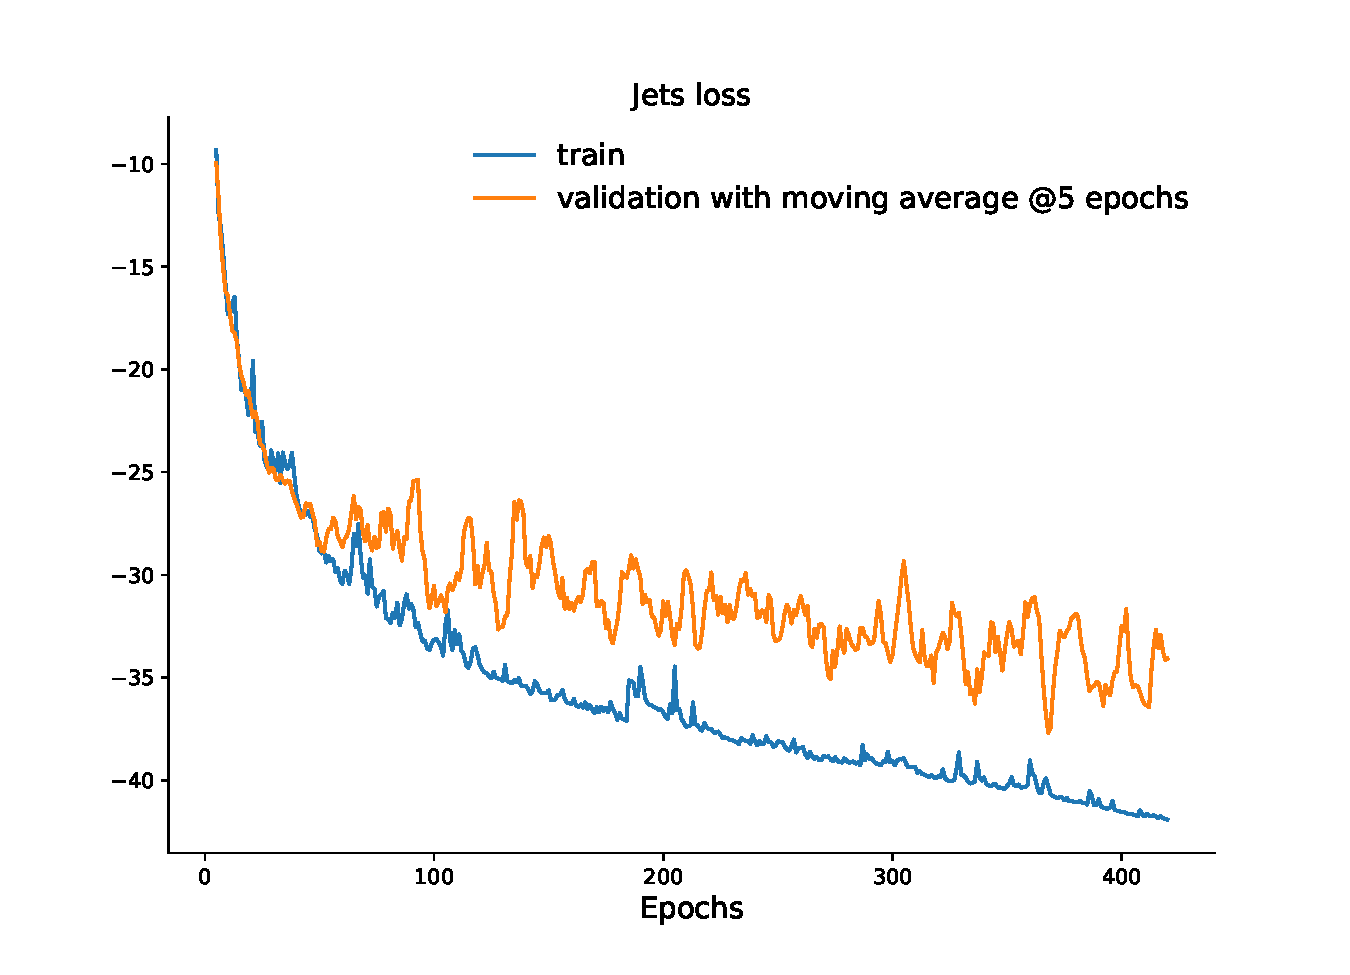
\includegraphics[width=\linewidth]{gfx/ch5/lossesjets.pdf}} 
    \caption[Models losses]{The training for both models (a muons and b jets) has reached a good convergence, but there is still room for improvements. The losses are plotted starting from epoch 5 to better display the decrease in the final epochs.}\label{fig:losses}
    
\end{figure}

We trained the models on the local INFN Pisa computing resources, specifically on a \texttt{NVIDIA V100} GPU with 32GB of VRAM and 5,120 CUDA Cores. The time spent for the training of both models was $\approx$ 5 days, however we observed that due to inefficient \emph{data loading} on the GPU, the maximum usage of the device fluctuated between 40$\%$ and 80$\%$ most of the time, indicating that more data loading resources or a different training scheme (such as \emph{distributed training}) could improve training times decisively.

\section{Results}

\graffito{do we want to plot the full results in an appendix?? or refer to a colab??}
We move on to discuss the results obtained. 
To perform a sound and reasonable comparison, we extract the Gen-values for conditioning from 1e5 samples coming from an unseen test set for jets and from the validation set (which was not used for training but just for evaluating the loss over time) for muons. We then generate new FlashSim samples starting from the same Gen-values, to get a one-to-one correspondence between the two sample sets.
It has been observed that when generating a larger number of events, in the order of millions to billions, low probability mass regions can produce negative, nonphysical values. This phenomenon is very rare and can be easily corrected by implementing a check in the postprocessing, regenerating the event through the extraction of new noise values to sample from a different region of the learned pdf.

There are two main types of comparison which can now be performed on the obtained samples: we can compare the \emph{distribution} or the \emph{correlations} for the two.
While the latter can be inspected visually thanks to \emph{contour plots}, we would like to define a precise measure for the similarity of the empirical distributions between two samples. We thus define the \emph{Wasserstein distance} as:

\[W_1(u, v) = \inf_{\pi \in \Gamma(u, v)}\int_{\mathbb{R}\times\mathbb{R}}\abs{x-y}d\pi(x,y) = \int_{-\infty}^{+\infty} \abs{U - V}\]

where $\Gamma(u, v)$ is the set of (probability) distributions on $\mathbb{R}\times\mathbb{R}$ whose marginals are $u$ and $v$ on the first and second factors respectively, and $U$, $V$ are the respective CDFs. Intuitively, if each distribution is viewed as a unit amount of earth (soil), the metric is the minimum \emph{cost} of turning one pile into the other, which is assumed to be the amount of earth that needs to be moved times the mean distance it has to be moved, and thus this metric is also know informally as the \emph{earth mover distance}.

\subsection{1d distributions and correlations}


\paragraph{Jets}

We show in Figure \ref{fig:jetsdists} four 1-d distributions from the total of 17 target variables obtained for jets. We emphasize once more that the model actually learned to generate the 17 values simultaneously, preserving the correct correlations as well as producing convincing distribution.

Regarding the distributions, we observe that the model has correctly learned all the multi-modal, sharply peaked tagging distributions with Wasserstein scores of the order of 1e-3, testifying good convergence. The log scale of \texttt{btagDeepB} actually shows an instance of \emph{bridging}, where a small set of values were generated between two separate peaks. Single-mode distributions such as \texttt{ptRatio} have been larned as well, as were the Ids thanks to dequantization. The \texttt{jetId} plot in log-scale actually shows that a small set of samples has been generated in the empty regions between values 0, 2 and 6 (the only admissible ones) but this is because the continuous output of the network has been rounded to the nearest integer. A more refined version of post-processing is expected to correct this behaviour.

Finally, we also observe a worse performance on two distributions: \texttt{bRegCorr}, a rather simple, skewed one-mode distribution which is expected to improve with further training (current Wasserstein distance is $\approx$ 0.02), and \texttt{nConstituents}, plotted at the bottom of \ref{fig:jetsdists}. The latter result is probably in stronger disagreement because the target actually consist of integer values--as we discussed before, the NF approach expects continuous distributions, and so the model performs bridging in an attempt to obtain a reasonable continuous distribution. However, it has been observed in previous training for similar architerctures that the model is actually capable of overcoming this limitation by brute force alone: if left in training for long enough it will eventually learn to reproduce the discrete peaks of the target.

\begin{figure}
    \myfloatalign
    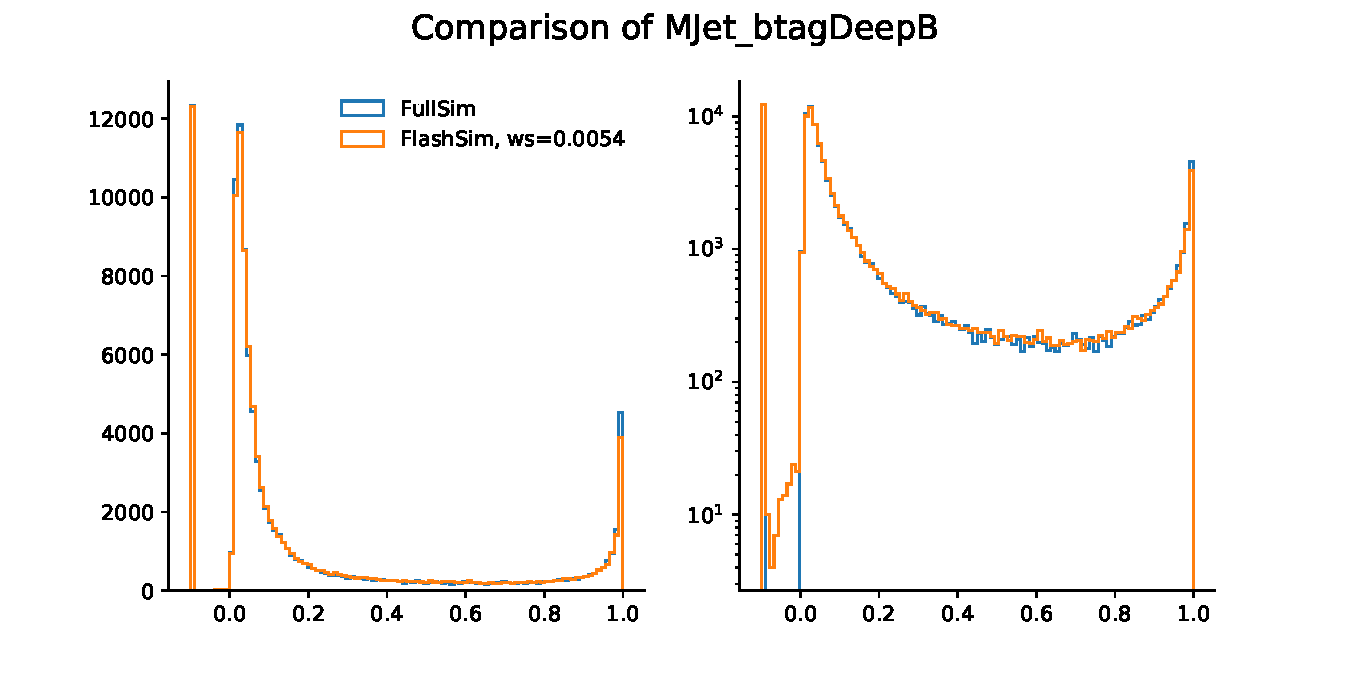
\includegraphics[width=\linewidth]{gfx/ch5/eval3.pdf} \\
    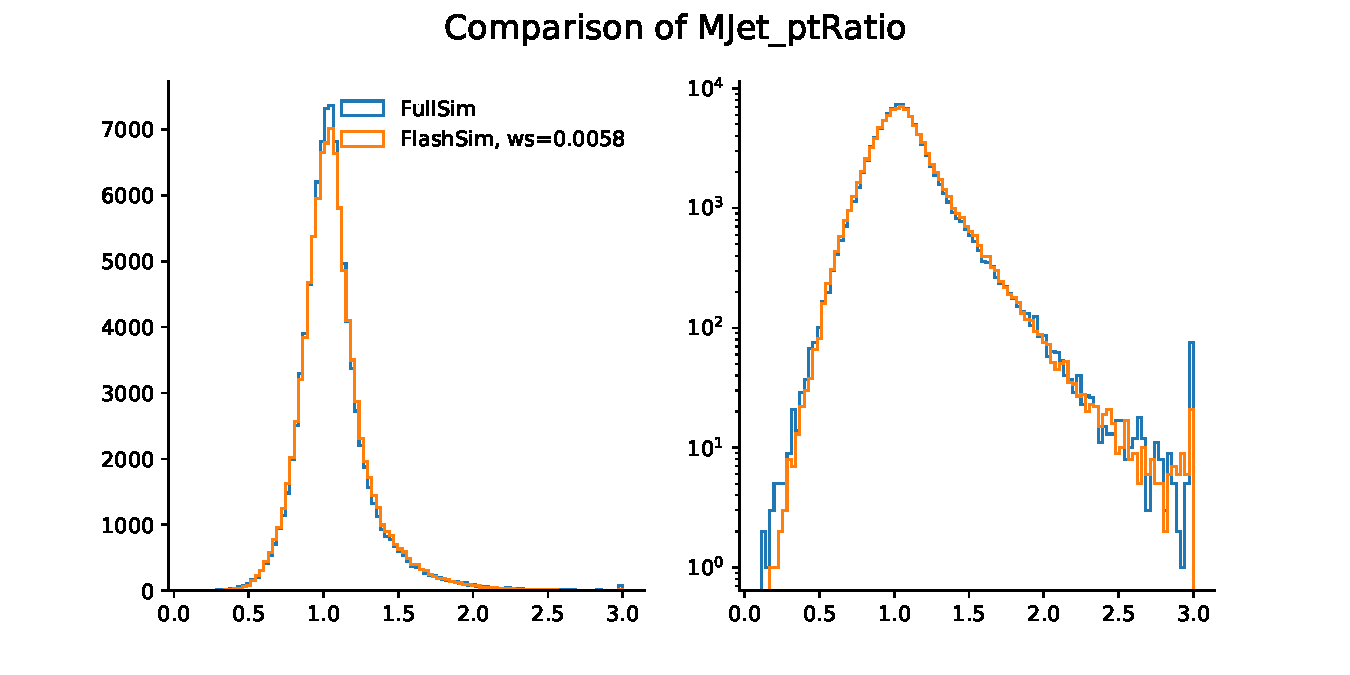
\includegraphics[width=\linewidth]{gfx/ch5/eval12.pdf} \\
    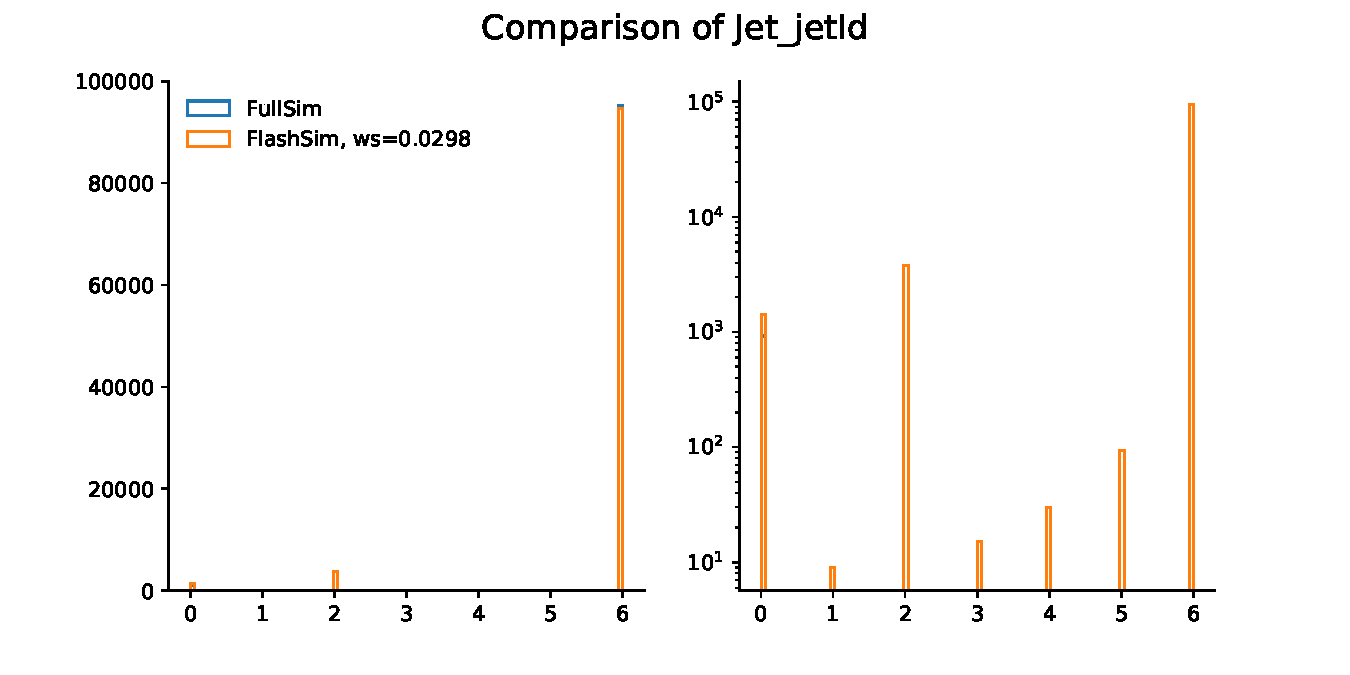
\includegraphics[width=\linewidth]{gfx/ch5/eval16.pdf} \\
    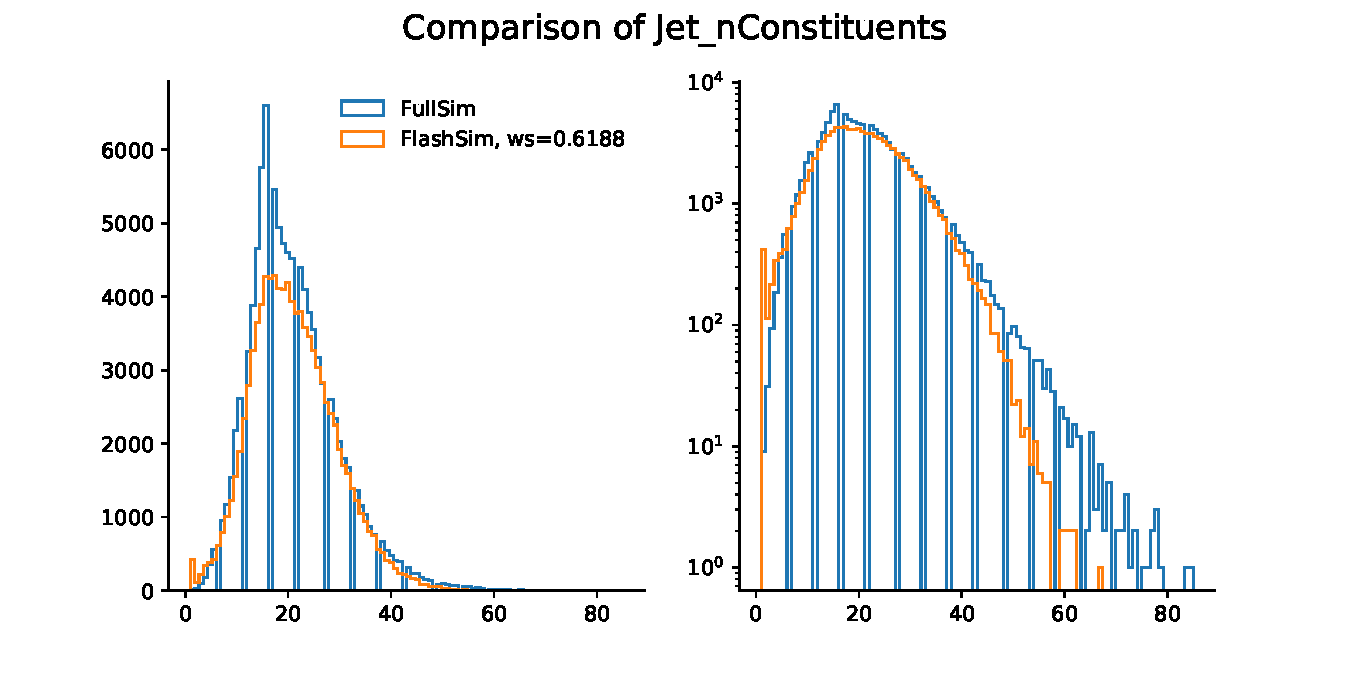
\includegraphics[width=\linewidth]{gfx/ch5/eval10.pdf}
    \caption[1-d jets distributions]{Four examples of 1-d distributions for jets. The model captures well multi-modal, sharply peaked distributions as well as single-mode, heavy tailed ones, and can also approximate Ids well thanks to dequantization. As expected it struggles with integers values such as \texttt{nConstituents}.}\label{fig:jetsdists}
    
\end{figure}

The correlations between jets variables, inspected visually, show good agreement with those from FullSim. Figure \ref{fig:corrjet1} shows the highly non-trivial correlations between the tagging distributions, with \emph{quantiles} plotted at 0.5, 0.9, 0.99. The same choice for quantiles has been adopted for all the following figures.

\begin{figure}
    \centering
    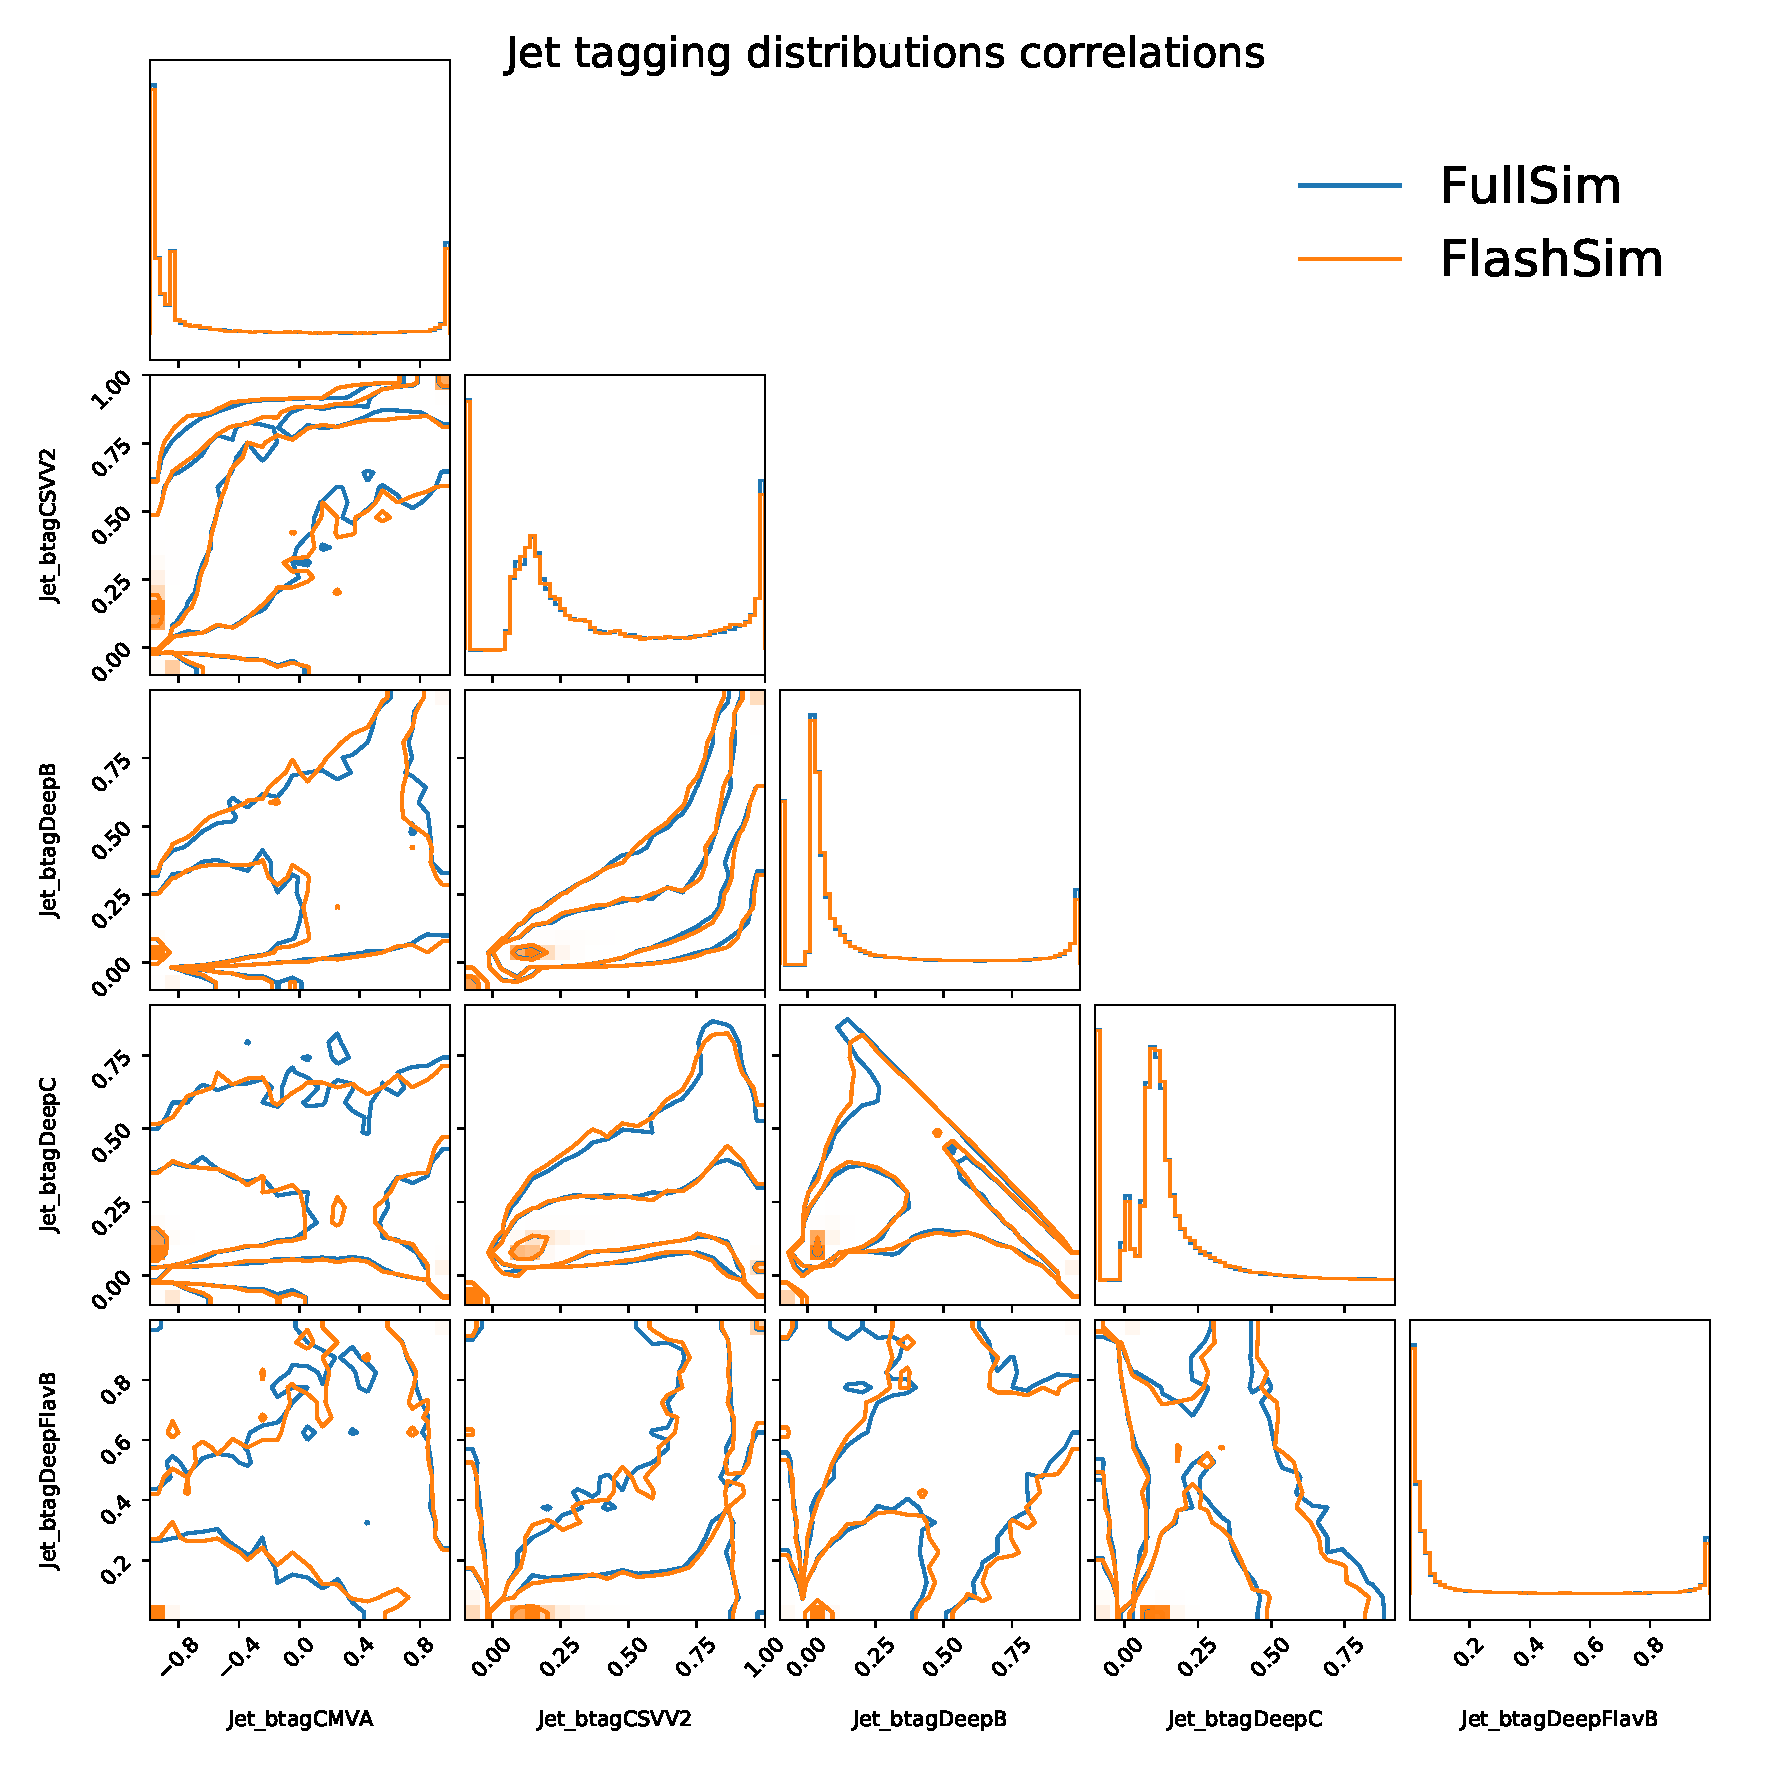
\includegraphics[width=\linewidth]{gfx/ch5/corrjet1.pdf}
    \caption[Tagging correlations]{Even non-trivial correlation such as the ones between tagging distributions are captured correctly by our models.}
    \label{fig:corrjet1}
\end{figure}

\graffito{get qgl nconstituens corr straight}
We can also observe in Figure \ref{fig:corrjet2+3} how the models have learned to capture the correlations between the qgl score, which is correctly correlated to the number of constituents as a lower number of constituents is expected for the u, d, s quarks when compared to gluons. Additionally, correlations between the physical p$_T$ and mass distributions, obtained from the original p$_T$Ratio and massRatio outputs of the network, are learned as well.

\begin{figure}
    \myfloatalign
    \subfloat[]
    {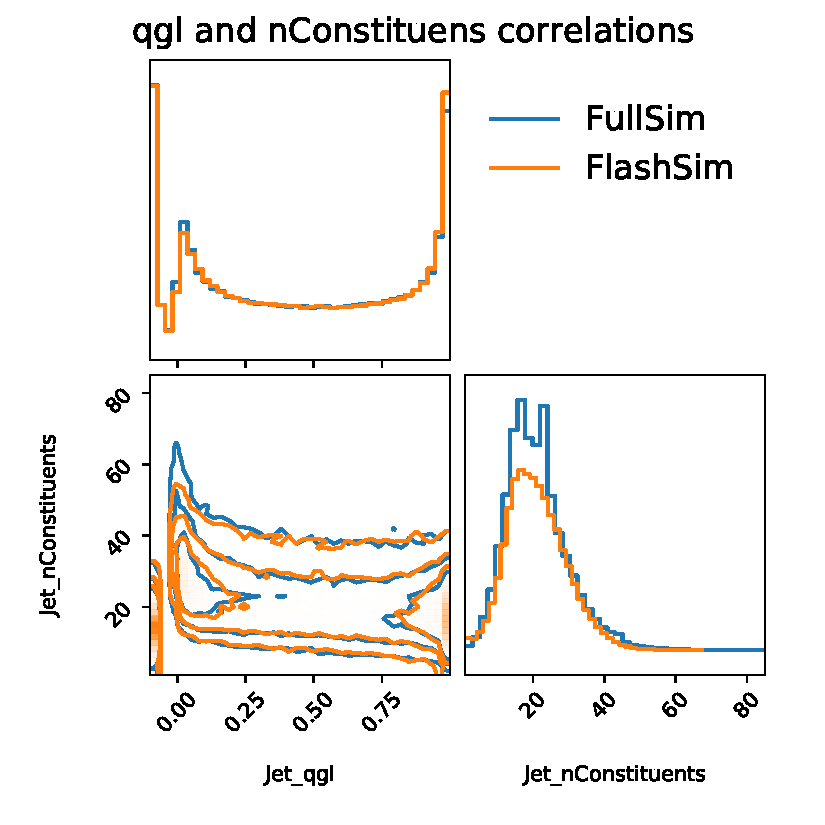
\includegraphics[width=0.45\linewidth]{gfx/ch5/corrjet2.pdf}}
    \subfloat[]
    { 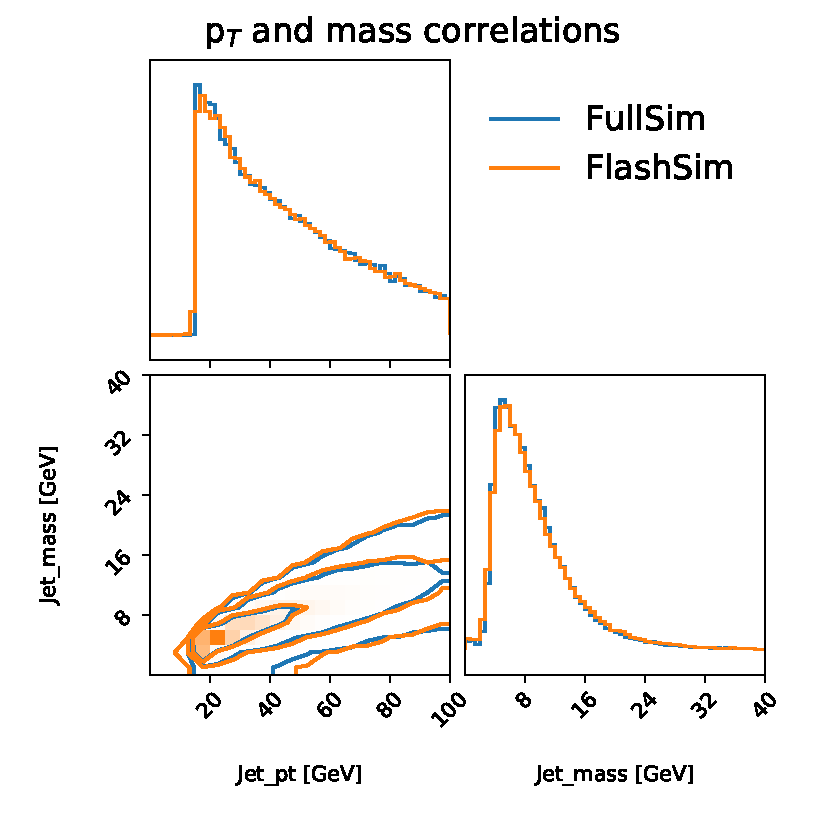
\includegraphics[width=0.45\linewidth]{gfx/ch5/corrjet3.pdf}} 
    \caption[qgl and p$_T$ correlations]{ (a) As expected, the qgl is positively correlated to the number of constituents--the lower the number, the larger the score. This behaviour has been captured by Flash Sim as well. The FullSim nConstituens distribution is jagged because of its discrete values, while the FlashSim has \emph{bridged} them and is thus smoothed.(b) The correlations between the physical distributions of p$_T$ and mass show agreement as well.}\label{fig:corrjet2+3}
    
\end{figure}

\paragraph{Muons}

For the muons, we obtained similar results--good, convincing general convergence and correlations apart from a subset of the target variable. It should be noted that a larger number of target variables for this case were actually Boolean Ids, and as discussed before were approached through dequantization. Figure \ref{fig:muonsdists} shows 4 distributions out of 22 target variables. Aside from good convergence on the firs two, we can observe that for a series of them, such as \texttt{dxyErr} and \texttt{dzErr} the training is complicated by the fact that the NanoAOD format stores the variables in a low-precision format: this is reflected by the jagged structure in the plot for FullSim and it causes the model to perform bridging to reach convergence.

\begin{figure}
    \myfloatalign
    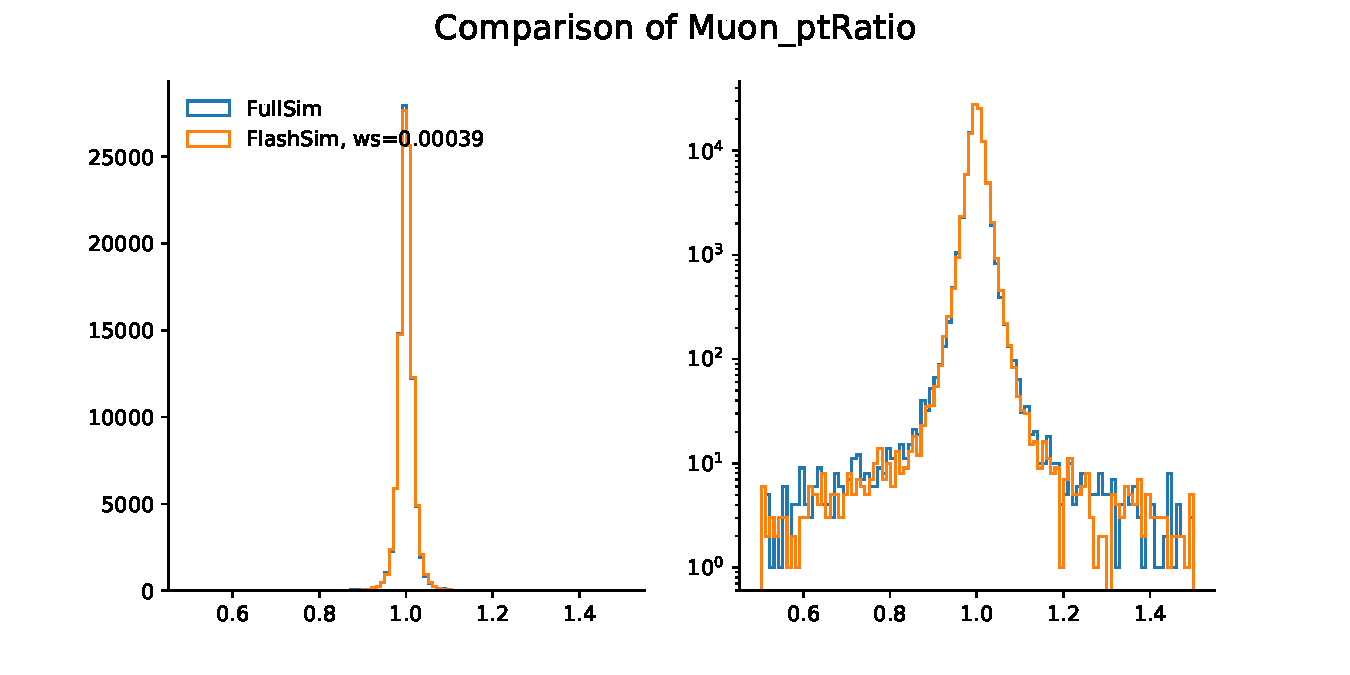
\includegraphics[width=\linewidth]{gfx/ch5/meval2.pdf} \\
    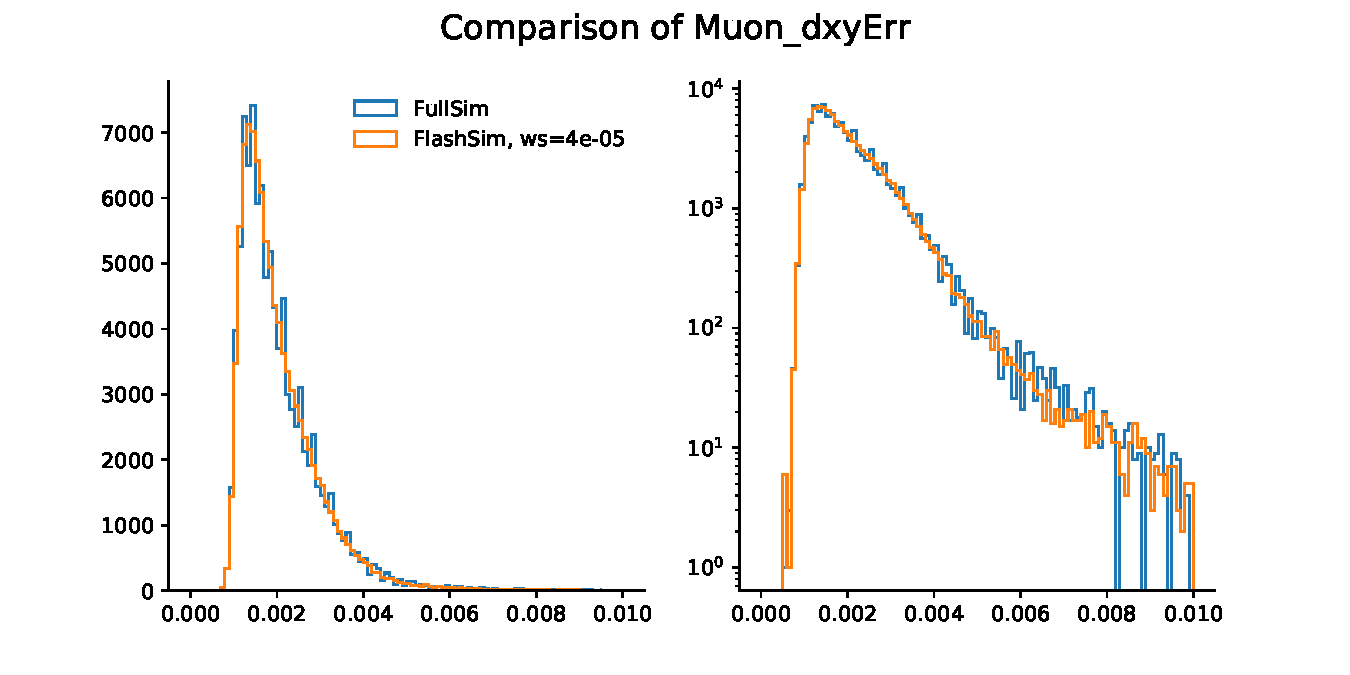
\includegraphics[width=\linewidth]{gfx/ch5/meval4.pdf} \\
    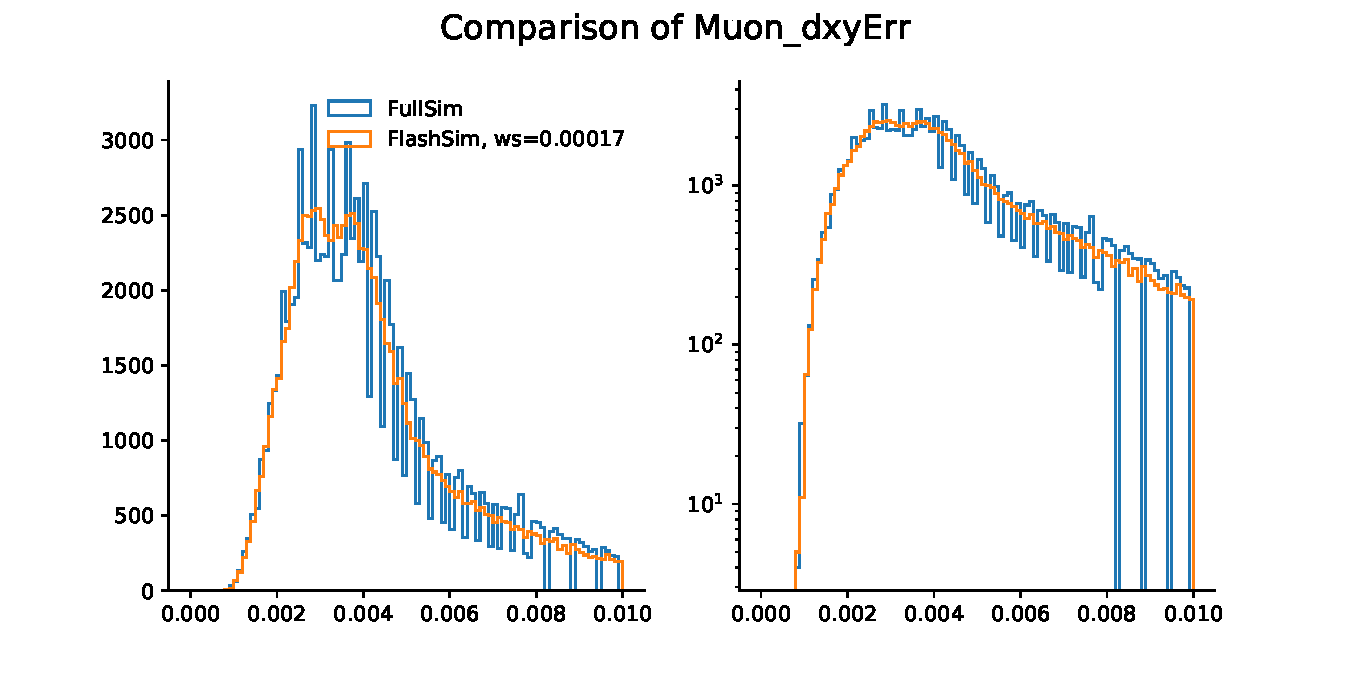
\includegraphics[width=\linewidth]{gfx/ch5/meval6.pdf} \\
    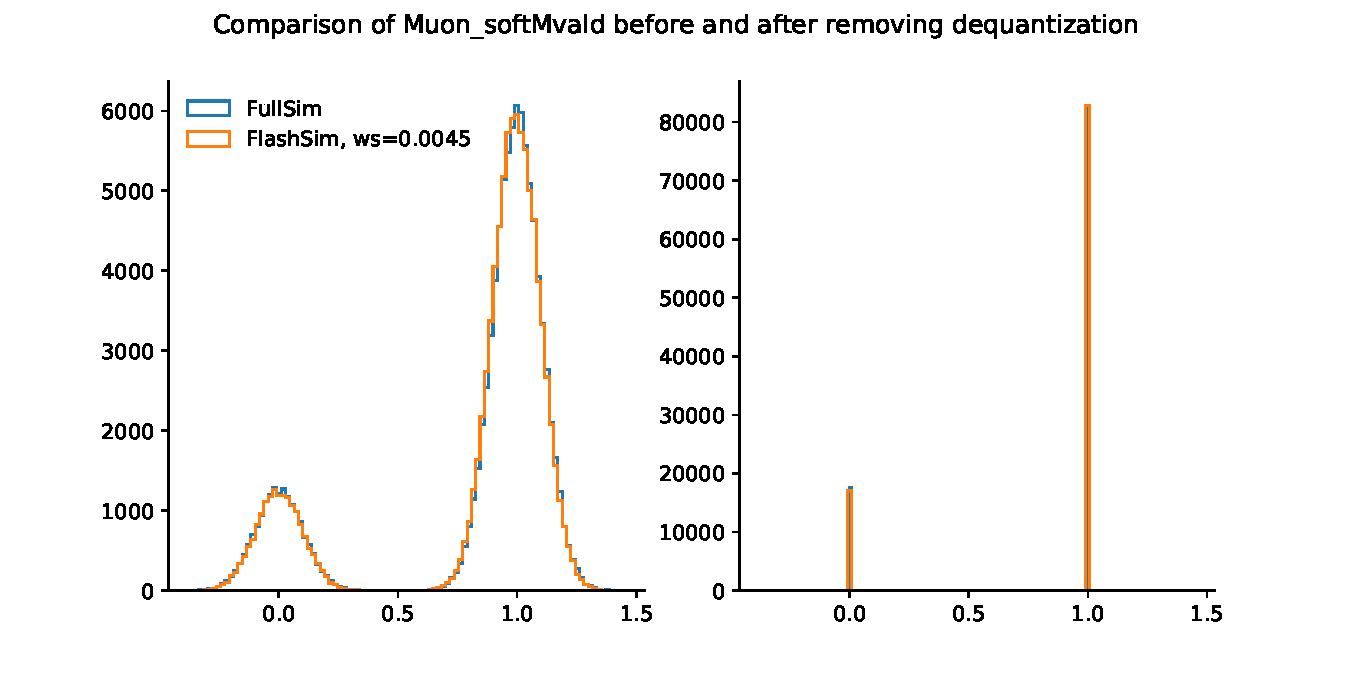
\includegraphics[width=\linewidth]{gfx/ch5/meval21.pdf}
    \caption[1-d muons distributions]{Four examples of 1-d distributions for muons. For most distributions the results present a small Wasserstein distance, however the model performs bridging in the presence of low-precision variables which present discrete peaks in the original FullSim..}\label{fig:muonsdists}
    
\end{figure}

\graffito{which is the exact relationship between ip3d and the sqrt?}
Finally, as a last example of correlations, we show in Figure \ref{fig:corrmuons} that the model has actually learned to capture complex correlations such as the ones between the \emph{impact parameter} \texttt{ip3d} and the quantity $\sqrt{\texttt{dxy}^2 + \texttt{dz}^2}$, which is closely related to the definition of the impact parameter itself.

\begin{figure}
    \centering
    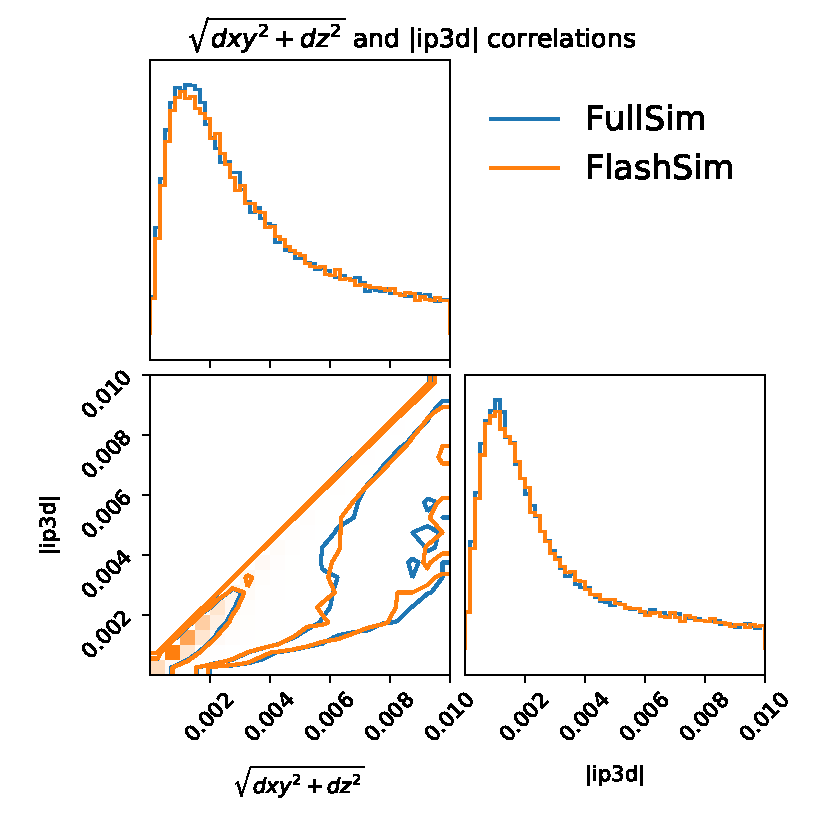
\includegraphics[scale=0.6]{gfx/ch5/mcorrs.pdf}
    \caption[Muons correlations]{The complex correlations between the \emph{impact parameters} \texttt{ip3d} and the related quantity $\sqrt{\texttt{dxy}^2 + \texttt{dz}^2}$ have been captured as well.}
    \label{fig:corrmuons}
\end{figure}


\subsection{Conditioning}

Another extremely important feature of our approach is the desired ability to obtain specific results starting from certain Gen-level inputs, a characteristic we called conditioning. 

We can readily see that this is possible by focusing on specific results obtained for the jets model. Figure \ref{fig:condit} shows that the final, NanoAOD level reconstructed p$_T$ is correctly correlated to the GenJet p$_T$ for both FullSim and FlashSim: as we would expect the Gen-p$_T$ is crucial in determining the final-state p$_T$. What is more, in the same figure we also show the \emph{profile histogram} and RMS ($\sigma_{p_T}$/p$_T$) for the GenJet p$_T$ versus the p$_T$Ratio. As expected, not only does the p$_T$Ratio decrease as the GenJet p$_T$ increases (highly energetic jets have a reconstructed p$_T$ closer to the Gen-value), but the RMS correctly decreases as well, as constant terms in the p$_T$ resolution due to PileUp are divided by bigger terms as GenJet p$_T$ increases.

\begin{figure}
    \myfloatalign
    \subfloat[]
    {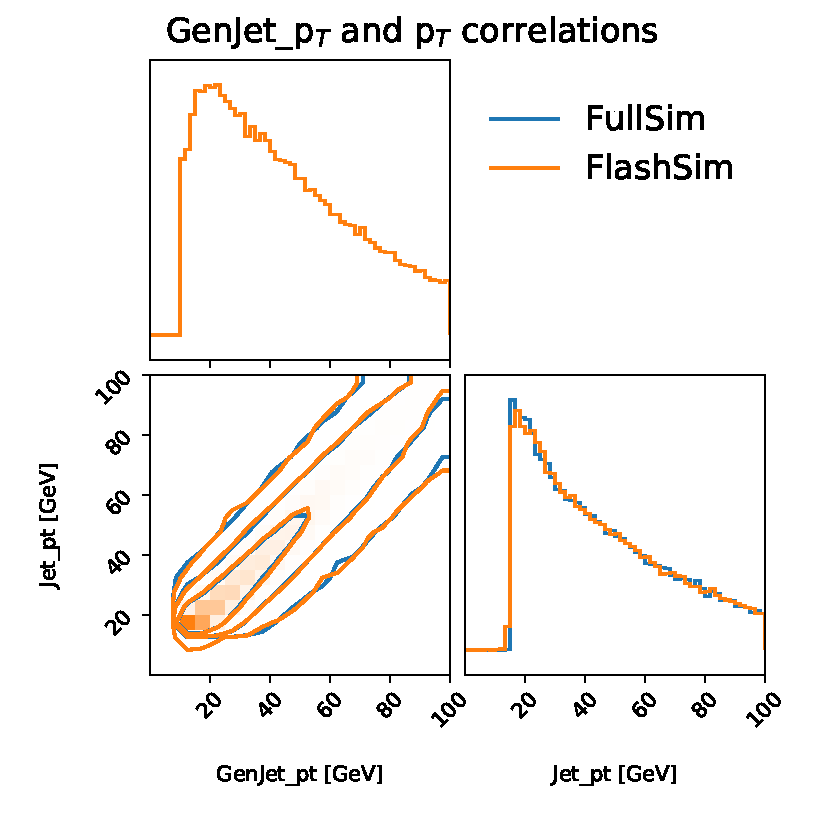
\includegraphics[width=0.45\linewidth]{gfx/ch5/corrjet4.pdf}}
    \subfloat[]
    { 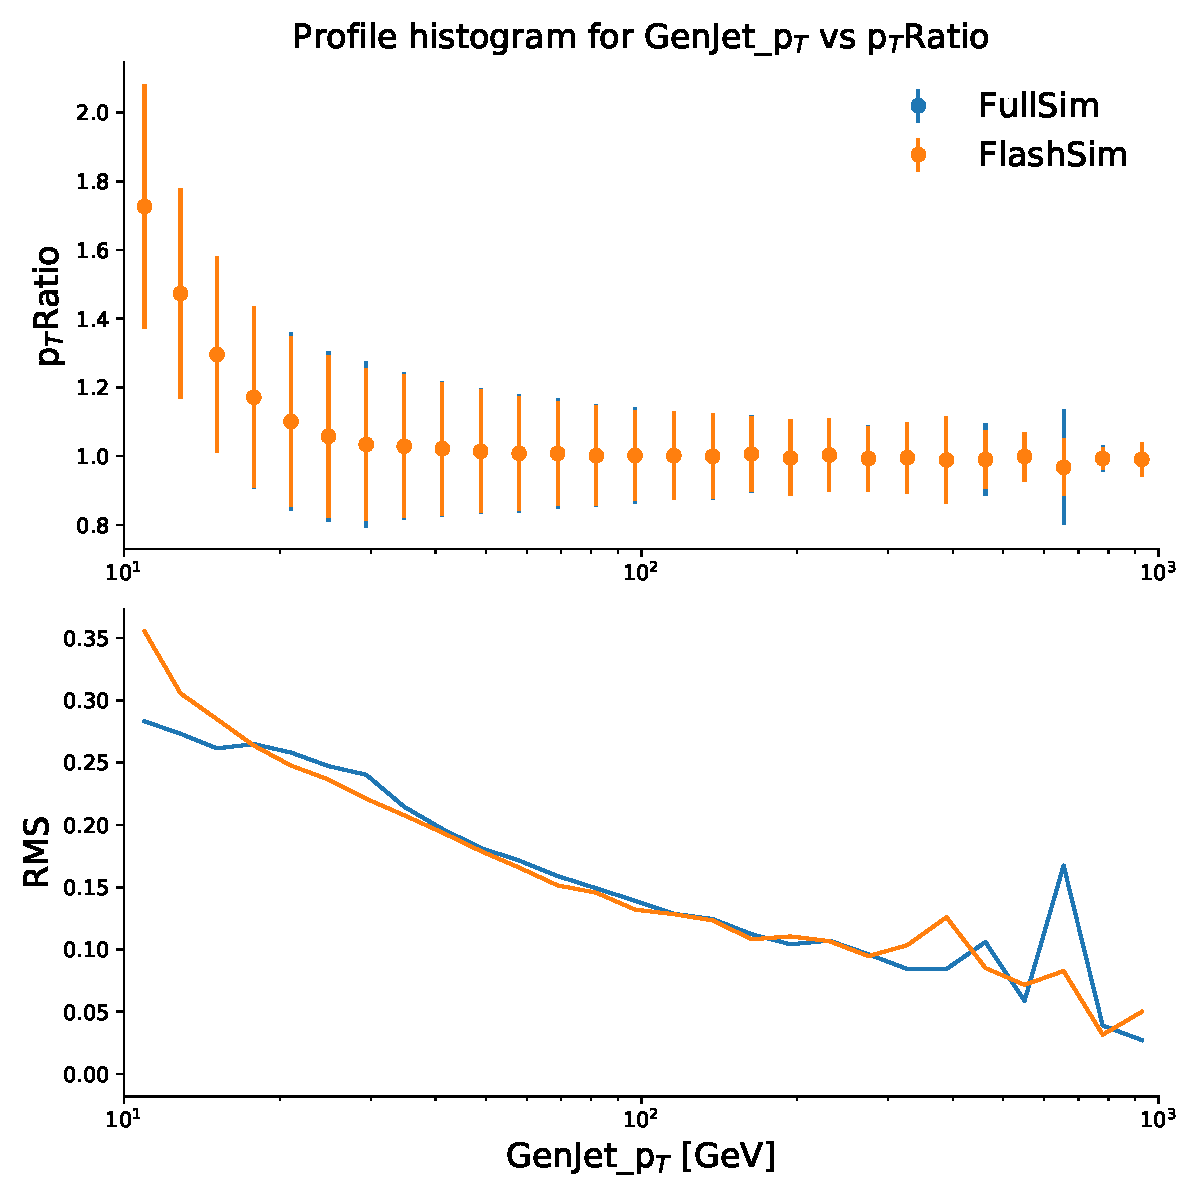
\includegraphics[width=0.45\linewidth]{gfx/ch5/profhist.pdf}} 
    \caption[Conditioning]{ (a) As we would expect the Gen-p$_T$ is crucial in determining the final-state p$_T$. Higher Gen-values correspond to higher reco-values. (b) Not only does the p$_T$Ratio decrease as the GenJet p$_T$ increases (highly energetic jets have a reconstructed p$_T$ closer to the Gen-value), but the RMS correctly decreases as well because of constant error terms being divided by larger Gen-values.}\label{fig:condit}
    
\end{figure}

Additionally, because the \texttt{partonFlavour} conditioning variable allow us to specify the quark content of a jet, we can study how related quantities depend on this input. As a key example, we study the behaviour of the \texttt{btagDeepB} b-tagging distribution as we vary the parton input for the jet generation. Figure \ref{fig:roc1} shows how the distribution changes according to the ground truth value specified as input: as expected, jets being conditioned with a b content present higher values of b-tagging, with a sharp peak at one, while those coming from u, d, s are clearly peaked aroun smaller values. Now we could think of defining a threshold and assign a reconstructed b content to all those jets higher than that value. We would naturally mistag some events, leading us to define a \emph{flase-positive} ratio and a \emph{true-positive} one. A standard figure of merit for these cases is the \emph{Receiving operating characteristic} curve, which plots the TPR against the FPR for all possible threshold choices. Figure \ref{fig:roc1} shows it for our model in log scale, showing minimal deviations from the target FullSim curve.


\begin{figure}
    \myfloatalign
    \subfloat[]
    {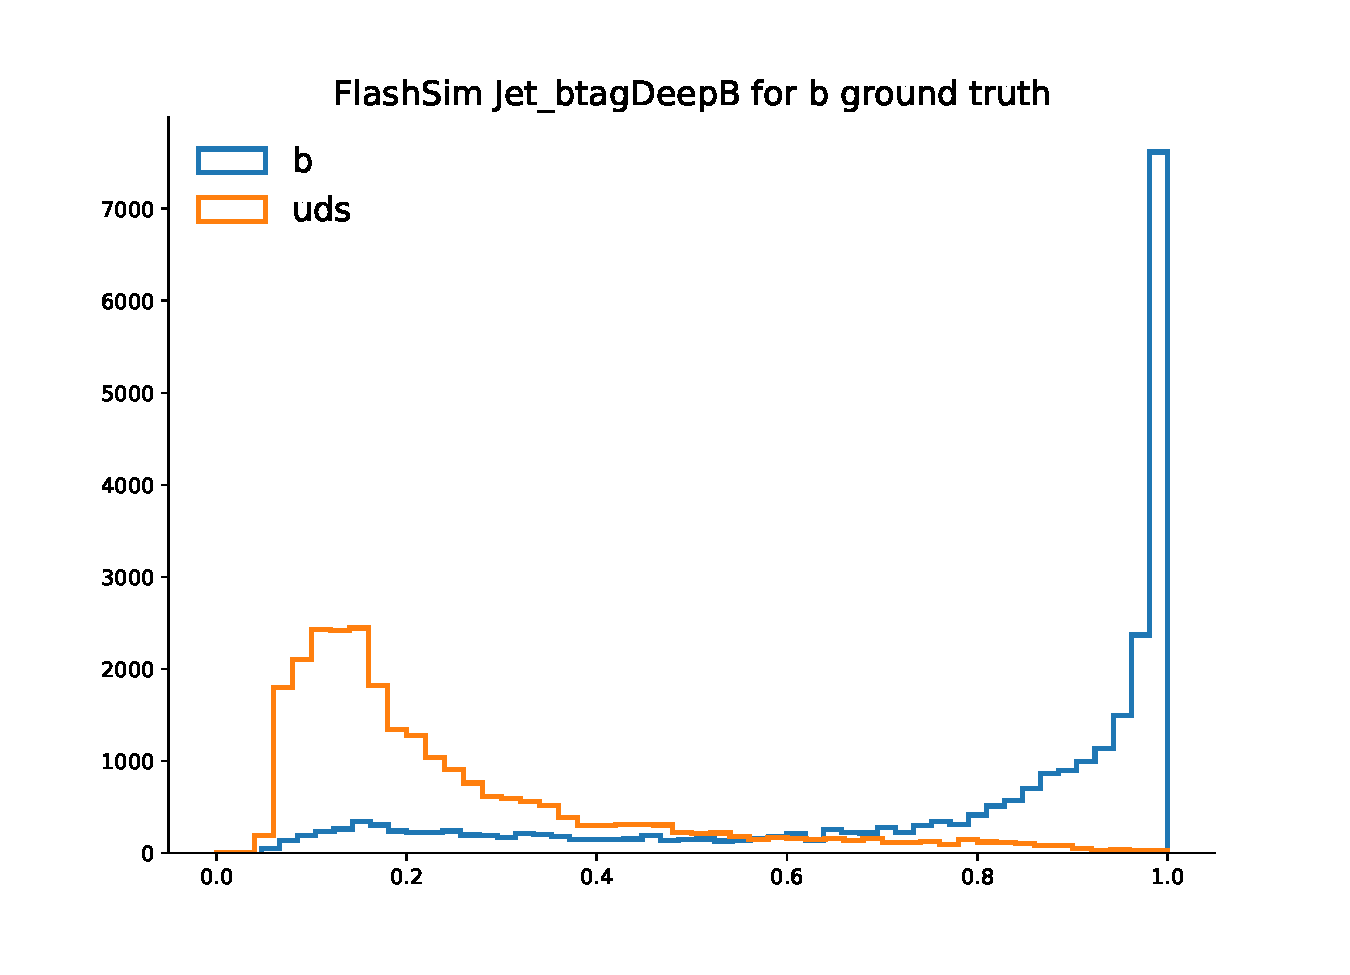
\includegraphics[width=0.45\linewidth]{gfx/ch5/btagj.pdf}}
    \subfloat[]
    { 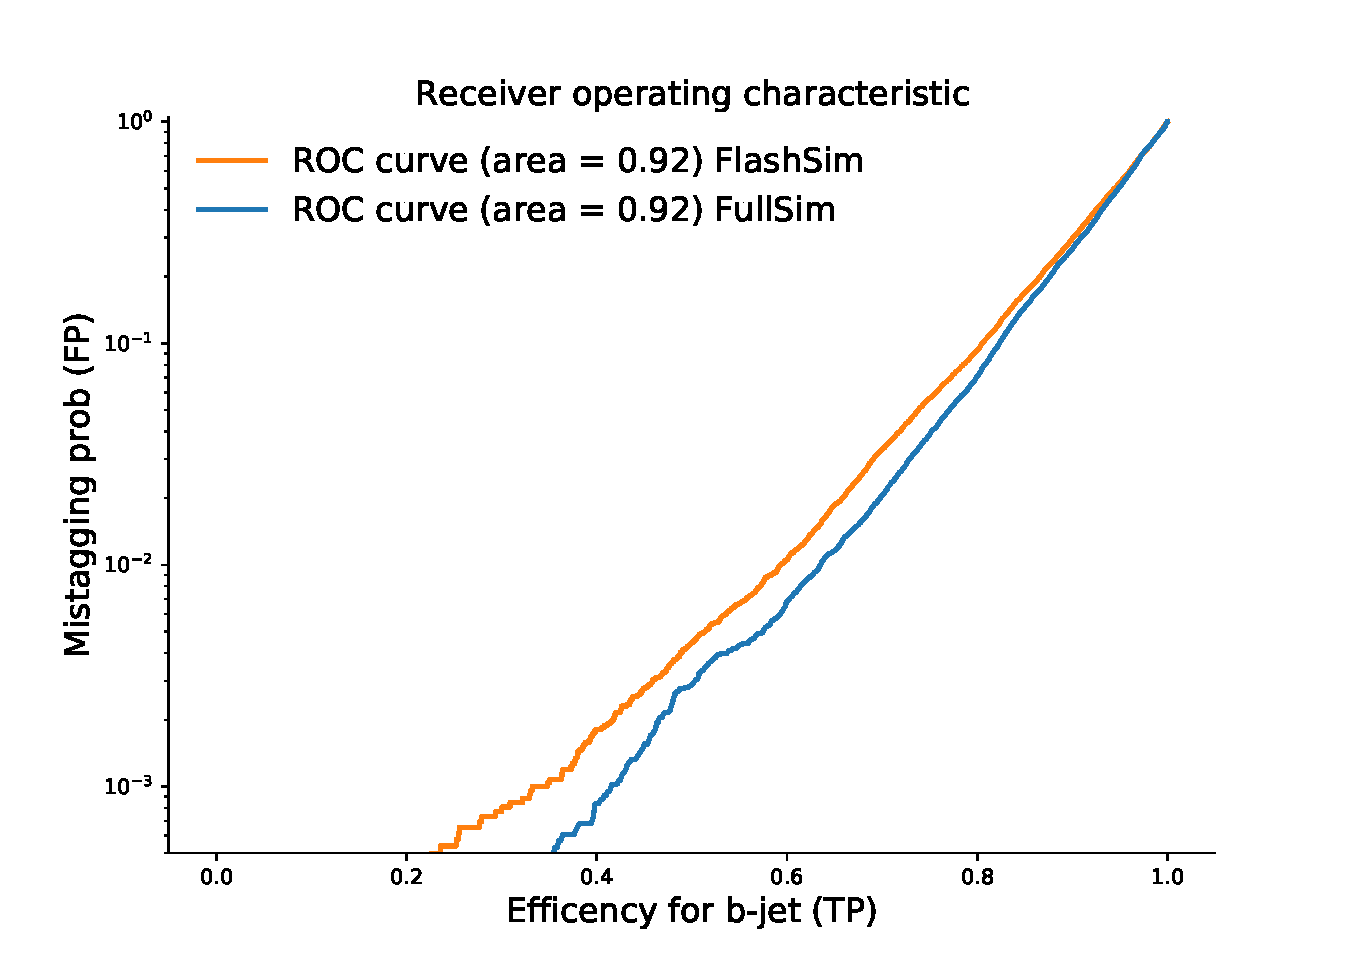
\includegraphics[width=0.45\linewidth]{gfx/ch5/roc.pdf}} 
    \caption[b-tagging and ROC]{ (a) The b-tagging distribution shape correctly depends upon the specified quark content at the Gen-level. (b) The ROC curve for the FlashSim approaches that for FullSim, showing that even on derived quantities our approach is capable of delivering satisfying results.}\label{fig:roc1}
    
\end{figure}

Because our results are not as close to FullSim as before, we would like to compare them with other competing approaches to asses the goodness of our own methodology. In order to do so, for a previous, simpler iteration of the jets model which was presented in the CMS Machine learning Forum of April 2022, we compared the ROC curves between FullSim, FastSim and FlashSim on a 1e6 samples set (not previously seen during training). Results are shown in Figure \ref{fig:allrocs} shows the comparison. We can see that while the ROC between our approach and FullSim is actually indistiguishable for TPR higher than 0.8, the FastSim ROC completely \emph{overshoots} the target, due to oversimplifications in the simulation approach. With longer training times and additional loss terms addressing this type of conditioning, we are confident that the performance of FlashSim could be improved even more.

\begin{figure}
    \centering
    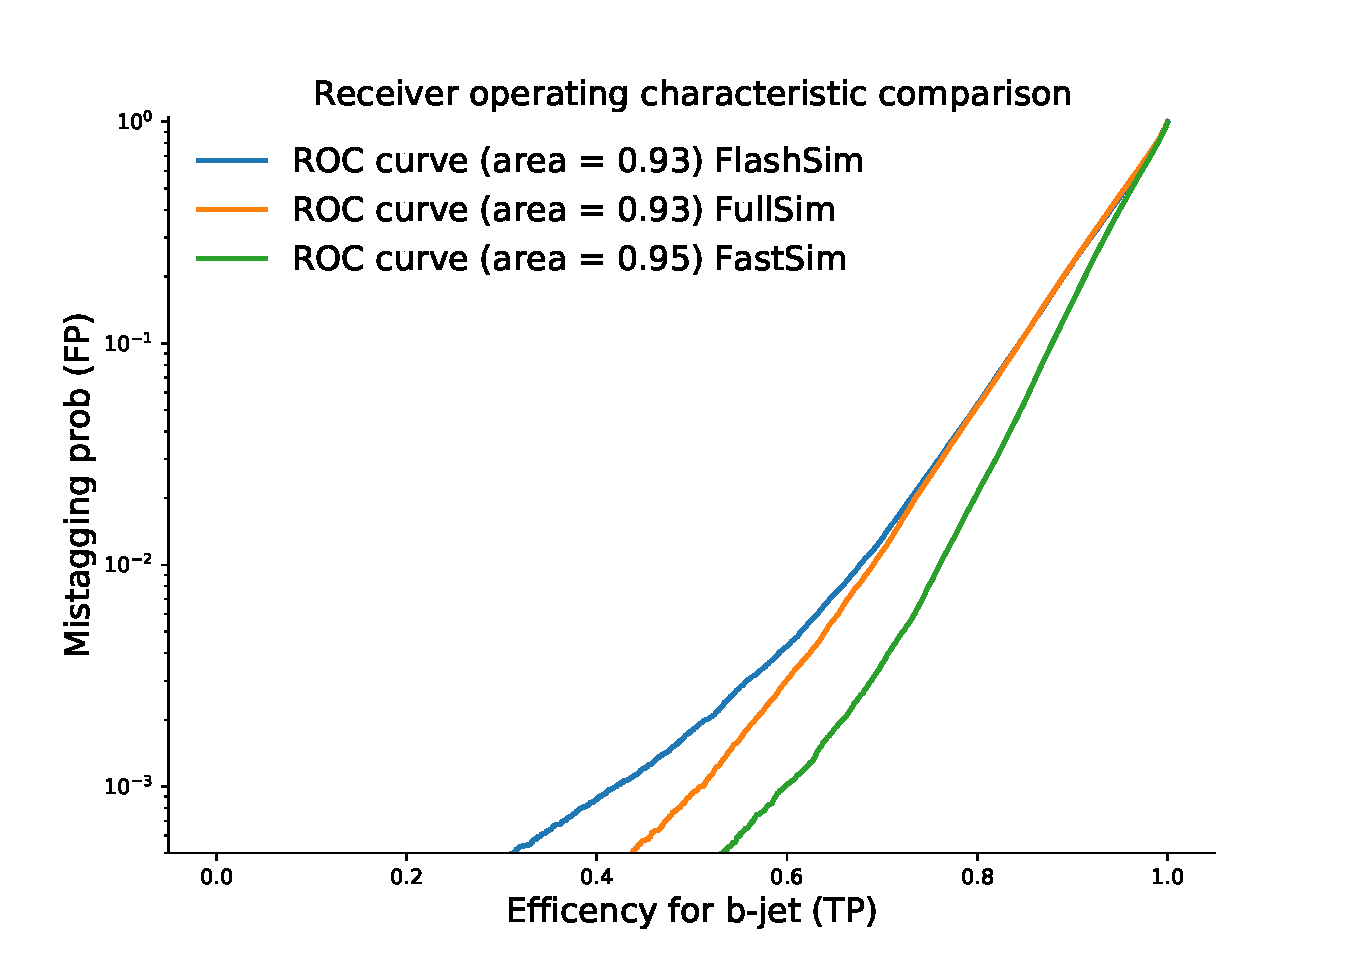
\includegraphics[width=\linewidth]{gfx/ch5/allrocs.pdf}
    \caption[ROC Comparison]{The FlashSim ROC can actually obtain close results to FullSim, while FastSim fails to replicate the target ROC.}
    \label{fig:allrocs}
\end{figure}


\subsection{Speed}

A crucial result obtained is the \emph{generation speed}: for both jets and muons we managed to generate samples in batches of 1e4 in $\approx$ 0.3 seconds each, corresponding to a generation speed of raw samples of about 33,300 \emph{samples per second} (33 kHz) \emph{meaning a six orders of magnitude speedup when compared to FullSim}! Even considering possible reduction due to preprocessing and data loading, this result testify to the potential of the current methodology to completely redefine our approach to event simulation, at least at the NanoAOD level.

What is more, the 1e4 batch size for generation was limited only by the VRAM of the GPU being used, meaning that more powerful GPUs, ideally working in parallel, could achieve even faster generation times.


\section{A prototype end-to-end analysis sample generator}\label{sec:progen}

We conclude by presenting the general idea for an end-to-end analysis sample generator in the NanoAOD format. The key concept can be easily grasped through Figure \ref{fig:endtoend}: a FullSim NanoAOD file gets processed and its Gen-level values extracted for eventual preprocessing. Then, the values are passed to the two networks, which generate raw samples which are finally postprocessed to reobtaine physical distributions and combined into a single, NanoAOD-like file format. The whole process can be executed by a single call to a \texttt{Python} script, which leverages the \texttt{ROOT C} interpreter for running the extraction and the \texttt{uproot} package for structuring and saving the data directly in the \texttt{.root} format, in a corresponding \texttt{TTree} data structure.

\begin{figure}
    \centering
    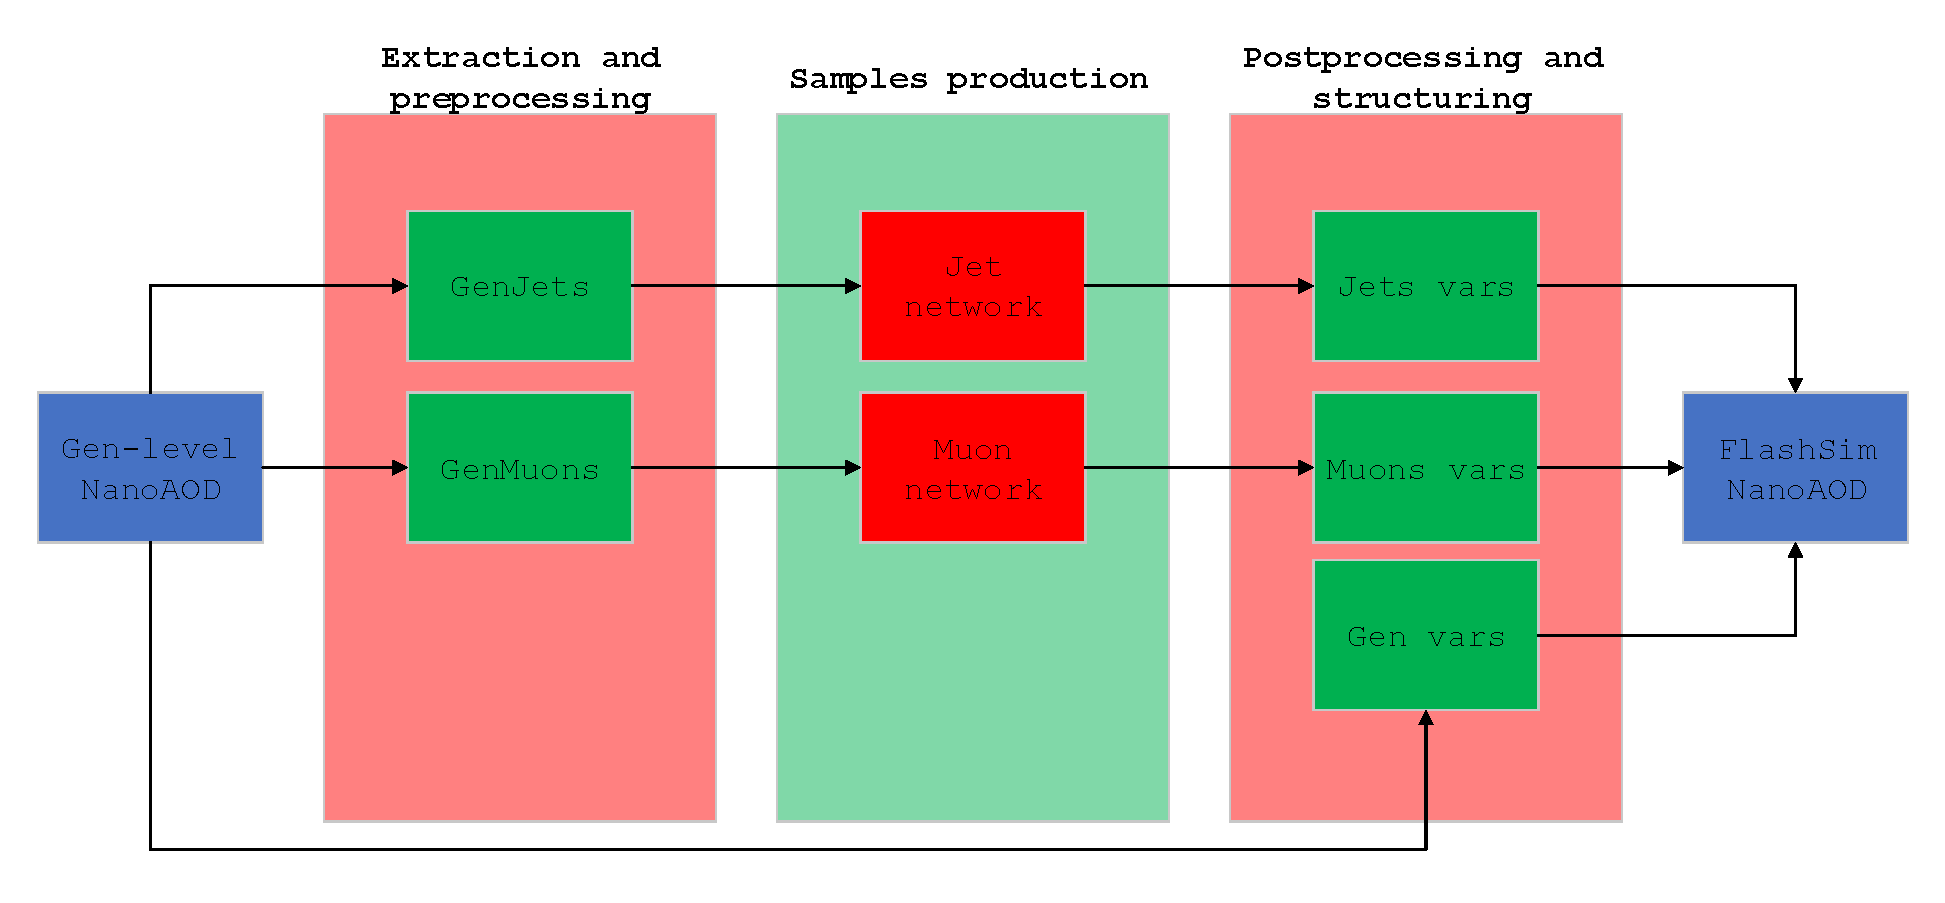
\includegraphics[width=\linewidth]{gfx/ch5/endtoend.pdf}
    \caption[end-toend sample generator]{The basic steps behind the prototype for an end-to-end sample generator.}
    \label{fig:endtoend}
\end{figure}

This prototype has been tested on the full \emph{TTJets} dataset (t$\overline{\text{t}}$ process) for the H$\rightarrow\mu^+\mu^-$ study of \cite{CMS-PAS-HIG-19-006}. What is more, we actually extended the use of the generator to \emph{different physical processes}: \emph{Drell-Yan}, \emph{Electroweak} and two \emph{Signal (H)} datasets were processed as well and stored for the comparison of the next chapter. The two signal datasets differ in the theoretical technique employed for \emph{systematic inclusion of higher order QCD effects}: one employed the \texttt{POWHEG} method \cite{Nason_2004}, the other the \texttt{MadGraph5\_aMC@NLO} \cite{powpow} one.
In total we processed more than 200 files, meaning several millions of events, in less than one day.

In the end, we proved that our networks can be integrated into the existing software base and can be used for obtaining files in the exact same standard of that used in current analysis at CMS. We were able to asses two major characteristics of our approach:

\begin{outline}
    \1 The NF networks are actually capable of tackling other processes, inherently different from the training one: both distributions and correlations maintain good accord with FullSim samples, despite considerable changes from the training set. This is a crucial property if we are to move away from the prototyping stage to a more realistic, full-scale and general-purpose NanoAOD simulator;
    \1 Considering the whole preprocessing/postprocessing/disk writing overhead, the whole process took about 440 second or 7 minutes on the typical NanoAOD file of the TTJets dataset (about 1e6 events per file), once again testyfing to the speed of the current methodology.
\end{outline}
%************************************************
\chapter{Conclusion and future outlook}\label{ch:outlook} % $\mathbb{ZNR}$
%************************************************
%************************************************
\chapter{Conclusion and future outlook}\label{ch:outlook} % $\mathbb{ZNR}$
%************************************************
In the present work, we introduced and implemented an alternative paradigm for the flash generation of events at the CMS experiment, based on state-of-the-art results from the ML field.

We were able to successfully simulate physical target distributions with great accuracy, preserving the correct correlations between them and demonstrating that our method is capable of varying the output results according to the physical information provided as input. This conditioning has been compared to that of the other competing approach for fast simulation, CMS FastSim, and has been shown to provide more accurate and precise results when compared with the original FullSim target for b-tag discrimination and jet $p_T$ resolution. Additionally, the proposed solution has demonstrated decisive advantages in terms of speed, with orders of magnitude of speed-up.

We also built a first prototype for an end-to-end sample generator in the standard CMS NanoAOD format, and actually deployed it at scale on millions of events, coming from the training process as well as new, previously unseen ones. 

Finally, we demonstrated that the results obtained can be used in a real world scenario such as a complex, multivariate, MC based analysis as the VBF Channel of H$\rightarrow\mu^+\mu^-$. We computed the key derived quantities for the analysis for both the FullSim and the FlashSim samples, and we observed comparable results on the evalutation of the DNN classifier used in the corresponding CMS publication.
Our approach was also able to provide interesting results regarding the generation of samples with different calculations of higher order QCD effects, being capable of reproducing the differences between competing approaches such as \texttt{POWHEG} and \texttt{MadGraph5\_aMC@NLO}.

\section{Towards a complete FlashSim}
This work has also emphasized some limitations and peculiarities of the selected approach, pointing to the next steps to be take if the CMS Collaboration were to adopt the proposed method.

The two major ones are discussed below.


\subsection{Building a full NanoAOD}
A full scale FlashSim must be able of reproducing the content of a NanoAOD file in its entirety. Due to the hundreds of variables stored in a single Event, the most reasonable approach is the one taken in the present work: instead of devising a massive single model for generating all the variables, it is better to divide the problem into a collection of separate physical objects, each reconstructed through its own network.

This has the clear advantage of reducing the size of the models and the resources needed for their trainings, beside, each single model may be conditioned on relevant quantities coming either from the Gen-level, from other model outputs or being specifically engineered to communicate key information regarding the event.

One crucial element for the production of convincing NanoAODs is the presence of \emph{fakes}. The stochastic nature of these objects make their production non-trivial, however there exist other techniques from the ML field, such as \emph{LSTM} \cite{lstm}, for handling and generation of variable-length sequences. The generation would depend on key quantities such as the PileUp and the GenParticles.

Another key quantity, the \emph{Missing Transverse Energy} (MET), could also depend on the final-state reconstructed objects, as this would allow us to obtain a more consistent description of the whole event.

A possible global picture, with multiple dependencies and conditionings, is illustrated in Figure \ref{fig:globpic}.

\begin{figure}
    \centering
    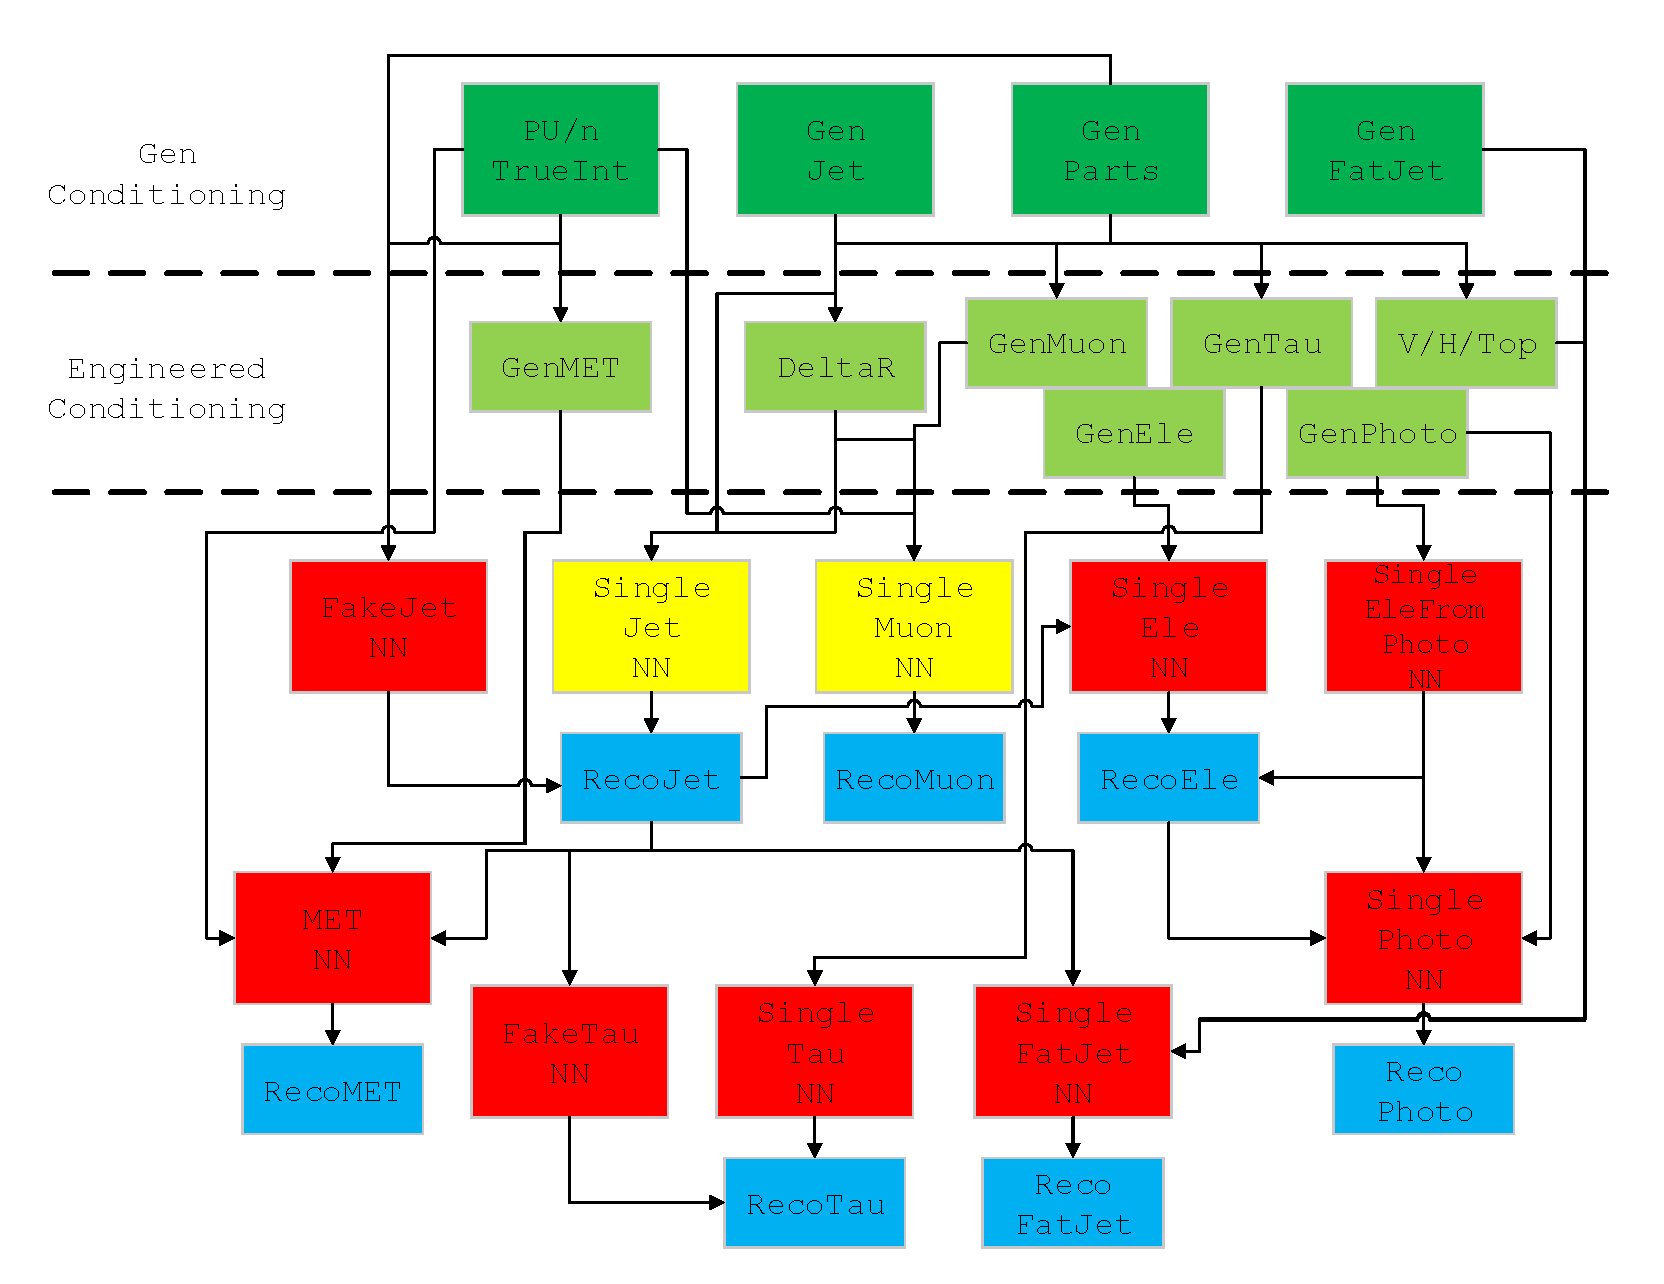
\includegraphics[width=\linewidth]{gfx/ch7/fullnanoaod.pdf}
    \caption[A global picture]{A possible global picture illustrating the various dependencies between conditioning, single object networks and RECO outputs.}
    \label{fig:globpic}
\end{figure}

\subsection{Optimization}
An important series of steps in the prototype end-to-end generator need to be optimized. 
First of all, the Gen-level quantities currently extracted from existing FullSim NanoAODs and written to file for processing could be produced from a dedicated FlashNano-Generator, capable of passing the desired inputs directly to our models without the need of previously existing files.

The ML models forming the backbone of our approach need to be properly optimized and thoroughly examined to find the best combination of hyperparameters, size and performance. Additionally, the training and the generation procedure may be modified to be run in parallel over multiple machines or clusters, providing significant speed advantages. Another very serious issue to be addressed by the collaboration is the fact that our research is based on a series of \texttt{Python} packages maintained by a series of open-source contributors with no interest in the specific HEP use case and no assurance of continued and prolonged support, as well as backward compatibility.

The issue may be addressed in several ways. A possibility would be to experiment with splines-based models such as ours with the current packages, but once found the optimal transformation, the splines and their parameters could be mapped into a more convenient \texttt{C/C++} framework to be used and actively maintained by one of the computing groups of CERN, and possibly integrated as part of the \texttt{ROOT} language.

Additionally, the postoprocessing step needs to be revised with the addition of a check for numerical instabilities causing nonphysical values for the target distributions. These may be then easily corrected by regenerating the faulty event with another set of random noise as input.

Finally, we could tailor a more specific loss function for our class of models, capable of taking in to account the goodness of the conditioning and evaluate how the physical-informed gen-inputs are driving the generation of the samples.

\section{Future research}
The need for fast and reliable computing methods in the physical sciences, notably in the high-energy field, has fueled much of the technological progress of modern times. Despite this, the average physicist has generally little time to spend on innovating and improving its computing toolkit, and has to content himself with boilerplate solutions. This is especially true in highly specialized fields, such as HEP, which purse a wide variety of research directions.

Specifically, in recent years, ML techniques have been massively adopted by scientific collaborations around the world. However, such tools remain geared towards the necessities of industry; much work remains to be done to enable the use of this technologies in hard sciences.

As physicists with a keen interest in this type of applications, while still retaining useful domain knowledge, we are convinced that significant results could be achieved by pursuing the following research directions. 

\subsection{Other Flow-based applications in HEP}

The versatility of Normalizing Flows make them an optimal choice for tackling a wide range of problems, namely all those where the definition and manipulation of \emph{pdf}s is of vital importance.

We already mentioned a series of possible approaches in Section \ref{sec:nfapp}. The most interesting is possibly the approach to \emph{anomaly detection}, where Flows have already been used to define empirical distributions from data (see \cite{Kasieczka_2021}). Other interesting approaches being currently tested and deployed at CERN make use of ML approaches as unbiased function approximants for unknown, empirical pdfs (e.g. \cite{D_Agnolo_2019}), however, perhaps being generally less known, NF have yet to be tested as a solution to the problem.

\subsection{Graph Networks and Normalizing Flows}

Possibly considered the holy grail of ML for HEP applications at the LHC, the problem of \emph{track reconstruction} is mostly a pattern recognition task whose complexity grows much more than linearly with the increase of number of collisions, hence the number of tracks, and is thus expected to be one of the main problems for HL-LHC. When investigating such a large feature space, a common approach is to reduce the complexity of the network while still retaining useful information about local features through the use of \emph{Convolutional Neural Networks} (CNNs), which nowadays are the standard approach for image datasets (as pioneered in \cite{simonyan2015deep}).
Unfortunately, any representation of tracking detector as images
would look very sparse and would not benefit of the locality idea of the CNN. 

Another hard HEP problem is the reconstruction of secondary vertices used for b-tagging. In order to identify b-jets, a useful feature is the presence of the so called \emph{secondary vertices} in a jet, i.e. points in space, displaced from the interaction point, where a group of tracks
appears to originate from.

A promising way to overcome these challenges is the introduction of \emph{Graph Networks} (GNs), which represent input and output data as graphs to exploit any invariance of the graph itself in order to perform the dimensionality reduction that is achieved in CNN. In the case of a GN, the locality is not based on an euclidean metric like as before, but rather on the number of connections needed to reach one node from another. In order to enforce this kind of locality, a \emph{Message Passing} schema is often used for GN: the computation happens in several iterations where each iteration propagates information to/from neighbor nodes. Even a simple overview of the method goes beyond the scope of this section: we will now comment briefly on specific HEP advantages of this architecture, referring the reader to the seminal work of Battaglia \emph{et al.} \cite{battaglia2018relational} for a comprehensive review.

The key idea behind GNs in HEP is to represent the data as a graph where the nodes are the hits (i.e. the individual measurements from tracking sensors) and nodes of subsequent layers are connected (with some pruning of nonphysical connections). The output is instead a graph made of several disconnected branches each representing an
individual track (or track seed). We would like to emphasize how a \emph{graph input topology} would possibly benefit many other models already in use at LHC, allowing a better application simply by performing a preprocessing step through the use of GN layers. An interesting work in this direction, proposing a new approach that considers a jet as an unordered set of its constituent particles, effectively a "particle cloud" is the one presented by Qu and Gouskos \cite{pj2020}. Based on the particle cloud representation, they proposed ParticleNet, a customized neural network architecture using Dynamic Graph Convolutional Neural Network for jet tagging problems. The ParticleNet architecture achieves state-of-the-art performance on two representative jet tagging benchmarks and is improved significantly over existing methods. 

The graph topology may be extended to the Normalizing Flow approach as well. The autors of \cite{https://doi.org/10.48550/arxiv.2105.09016} introduced \emph{Equivariant Normalizing Flows} based on graph networks as the building block for defining equivariant invertible functions acting on graphs and capable of translating the NF approach to the generation of molecular structures.

In a similar vein, we could imagine to generate graph structures representing our target particle cloud representation, paving the way for an entirely new and powerful simulation approach at a completely different level from what discussed in the present work.

\subsection{Quantum Machine Learning}

Finally, a novel discipline born from \emph{Quantum Computing} and ML, known as \emph{Quantum Machine Learning} (QML) is already under serious investigation from the scientific community, due to the potential and significant \emph{quantum} advantages. The limits of what machines can learn have always been defined by the computer hardware we run our algorithms on—for example, the success of modern-day deep learning with neural networks is enabled by parallel GPU clusters.

Quantum machine learning extends the pool of hardware for machine learning by an entirely new type of computing device—the \emph{quantum computer}. Some research focuses on ideal, universal quantum computers (“fault-tolerant QPUs”) which are still years away. But there is rapidly-growing interest in quantum machine learning on near-term quantum devices (\emph{Noisy Intermediate-Scale Quantum} or NISQ).

We can understand these devices as special-purpose hardware like Application-Specific Integrated Circuits (ASICs) and Field-Programmable Gate Arrays (FPGAs), which are more limited in their functionality but nonetheless well suited to specific applications. In the modern viewpoint, quantum computers can be used and trained like neural networks. We can systematically adapt the physical control parameters, such as an electromagnetic field strength or a laser pulse frequency, to solve a problem. Additionally, quantum circuits are differentiable, and a quantum computer itself can compute the change in control parameters needed to become better at a given task. Trainable quantum circuits can be leveraged in other fields like quantum chemistry or quantum optimization. It can help in a variety of applications such as the design of quantum algorithms, the discovery of quantum error correction schemes, and the understanding of physical systems.

At the moment the effort of the HEP community is focused on quantum generative models (see \cite{chan2021quantum}), where the noisy behavior is mitigated or even beneficial. The CERN has already established a partnership with IBM, a leading competitor for quantum technologies, and founded the CERN Quantum Technology Initiative (CERN QTI), a comprehensive R$\&$D, academic and knowledge-sharing initiative to exploit quantum advantage for high-energy physics and beyond. 
%\include{multiToC} % <--- just debug stuff, ignore for your documents
% ********************************************************************
% Backmatter
%*******************************************************
\appendix
%\renewcommand{\thechapter}{\alph{chapter}}
\cleardoublepage
\ctparttext{You can put some informational part preamble text here.
Illo principalmente su nos. Non message \emph{occidental} angloromanic
da. Debitas effortio simplificate sia se, auxiliar summarios da que,
se avantiate publicationes via. Pan in terra summarios, capital
interlingua se que. Al via multo esser specimen, campo responder que
da. Le usate medical addresses pro, europa origine sanctificate nos se.}
\part{Appendix}
%********************************************************************
% Appendix
%*******************************************************
% If problems with the headers: get headings in appendix etc. right
%\markboth{\spacedlowsmallcaps{Appendix}}{\spacedlowsmallcaps{Appendix}}
\chapter{Appendix Test}\label{ch:appx}
First of all, we point out to the interested reader that the final version of the code used in this Thesis is hosted and documented in detail online \href{tbd}{at the following repository}\footnote{repository link, tbd}.

%Errem omnium ea per, pro congue populo ornatus cu, ex qui dicant
%nemore melius. No pri diam iriure euismod. Graecis eleifend
%appellantur quo id. Id corpora inimicus nam, facer nonummy ne pro,
%kasd repudiandae ei mei. Mea menandri mediocrem dissentiet cu, ex
%nominati imperdiet nec, sea odio duis vocent ei. Tempor everti
%appareat cu ius, ridens audiam an qui, aliquid admodum conceptam ne
%qui. Vis ea melius nostrum, mel alienum euripidis eu.

\section{Appendix Section Test}
Test: \autoref{tab:moreexample} (This reference should have a
lowercase, small caps \spacedlowsmallcaps{A} if the option
\texttt{floatperchapter} is activated, just as in the table itself
 $\rightarrow$ however, this does not work at the moment.)

\begin{table}[h]
    \myfloatalign
    \begin{tabularx}{\textwidth}{Xll} \toprule
        \tableheadline{labitur bonorum pri no} & \tableheadline{que vista}
        & \tableheadline{human} \\ \midrule
        fastidii ea ius & germano &  demonstratea \\
        suscipit instructior & titulo & personas \\
        %postulant quo & westeuropee & sanctificatec \\
        \midrule
        quaestio philosophia & facto & demonstrated \\
        %autem vulputate ex & parola & romanic \\
        %usu mucius iisque & studio & sanctificatef \\
        \bottomrule
    \end{tabularx}
    \caption[Autem usu id]{Autem usu id.}
    \label{tab:moreexample}
\end{table}

%Nulla fastidii ea ius, exerci suscipit instructior te nam, in ullum
%postulant quo. Congue quaestio philosophia his at, sea odio autem
%vulputate ex. Cu usu mucius iisque voluptua. Sit maiorum propriae at,
%ea cum primis intellegat. Hinc cotidieque reprehendunt eu nec. Autem
%timeam deleniti usu id, in nec nibh altera.




\section{Another Appendix Section Test}
Equidem detraxit cu nam, vix eu delenit periculis. Eos ut vero
constituto, no vidit propriae complectitur sea. Diceret nonummy in
has, no qui eligendi recteque consetetur. Mel eu dictas suscipiantur,
et sed placerat oporteat. At ipsum electram mei, ad aeque atomorum
mea. There is also a useless Pascal listing below: \autoref{lst:useless}.

\begin{lstlisting}[float=b,language=Pascal,frame=tb,caption={A floating example (\texttt{listings} manual)},label=lst:useless]
for i:=maxint downto 0 do
begin
{ do nothing }
end;
\end{lstlisting}

%Ei solet nemore consectetuer nam. Ad eam porro impetus, te choro omnes
%evertitur mel. Molestie conclusionemque vel at, no qui omittam
%expetenda efficiendi. Eu quo nobis offendit, verterem scriptorem ne
%vix.


%********************************************************************
% Other Stuff in the Back
%*******************************************************
\cleardoublepage%********************************************************************
% Bibliography
%*******************************************************
% work-around to have small caps also here in the headline
% https://tex.stackexchange.com/questions/188126/wrong-header-in-bibliography-classicthesis
% Thanks to Enrico Gregorio
\defbibheading{bibintoc}[\bibname]{%
  \phantomsection
  \manualmark
  \markboth{\spacedlowsmallcaps{#1}}{\spacedlowsmallcaps{#1}}%
  \addtocontents{toc}{\protect\vspace{\beforebibskip}}%
  \addcontentsline{toc}{chapter}{\tocEntry{#1}}%
  \chapter*{#1}%
}
\printbibliography[heading=bibintoc]

% Old version, will be removed later
% work-around to have small caps also here in the headline
%\manualmark
%\markboth{\spacedlowsmallcaps{\bibname}}{\spacedlowsmallcaps{\bibname}} % work-around to have small caps also
%\phantomsection
%\refstepcounter{dummy}
%\addtocontents{toc}{\protect\vspace{\beforebibskip}} % to have the bib a bit from the rest in the toc
%\addcontentsline{toc}{chapter}{\tocEntry{\bibname}}
%\label{app:bibliography}
%\printbibliography

\cleardoublepage%*******************************************************
% Declaration
%*******************************************************
\pdfbookmark[0]{Declaration}{declaration}
\chapter*{Declaration}
\thispagestyle{empty}
Put your declaration here.
\bigskip

\noindent\textit{\myLocation, \myTime}

\smallskip

\begin{flushright}
    \begin{tabular}{m{5cm}}
        \\ \hline
        \centering\myName \\
    \end{tabular}
\end{flushright}

\cleardoublepage\pagestyle{empty}

\hfill

\vfill


\pdfbookmark[0]{Colophon}{colophon}
\section*{Colophon}
This document was typeset using the typographical look-and-feel \texttt{classicthesis} developed by Andr\'e Miede and Ivo Pletikosić.
The style was inspired by Robert Bringhurst's seminal book on typography ``\emph{The Elements of Typographic Style}''.
\texttt{classicthesis} is available for both \LaTeX\ and \mLyX:
\begin{center}
\url{https://bitbucket.org/amiede/classicthesis/}
\end{center}


\bigskip

\noindent\finalVersionString

%Hermann Zapf's \emph{Palatino} and \emph{Euler} type faces (Type~1 PostScript fonts \emph{URW
%Palladio L} and \emph{FPL}) are used. The ``typewriter'' text is typeset in \emph{Bera Mono},
%originally developed by Bitstream, Inc. as ``Bitstream Vera''. (Type~1 PostScript fonts were made
%available by Malte Rosenau and
%Ulrich Dirr.)

%\paragraph{note:} The custom size of the textblock was calculated
%using the directions given by Mr. Bringhurst (pages 26--29 and
%175/176). 10~pt Palatino needs  133.21~pt for the string
%``abcdefghijklmnopqrstuvwxyz''. This yields a good line length between
%24--26~pc (288--312~pt). Using a ``\emph{double square textblock}''
%with a 1:2 ratio this results in a textblock of 312:624~pt (which
%includes the headline in this design). A good alternative would be the
%``\emph{golden section textblock}'' with a ratio of 1:1.62, here
%312:505.44~pt. For comparison, \texttt{DIV9} of the \texttt{typearea}
%package results in a line length of 389~pt (32.4~pc), which is by far
%too long. However, this information will only be of interest for
%hardcore pseudo-typographers like me.%
%
%To make your own calculations, use the following commands and look up
%the corresponding lengths in the book:
%\begin{verbatim}
%    \settowidth{\abcd}{abcdefghijklmnopqrstuvwxyz}
%    \the\abcd\ % prints the value of the length
%\end{verbatim}
%Please see the file \texttt{classicthesis.sty} for some precalculated
%values for Palatino and Minion.
%
%    \settowidth{\abcd}{abcdefghijklmnopqrstuvwxyz}
%    \the\abcd\ % prints the value of the length

% ********************************************************************
% Game Over: Restore, Restart, or Quit?
%*******************************************************
\end{document}
% ********************************************************************
